%    minted language=cpp,

%%%%%%
%%%%%%%%%%%%%%%%%%%%%%%%%%%%%% Title Page Info %%%%%%%%%%%%%%%%%%%%%%%%%%%%%%%%%%%%%%%%%%%
%%%%%%%%%%%%%%%%%%%%%%%%%%%%%%%%%%%%%%%%%%%%%%%%%%%%%%%%%%%%%%%%%%%%%%%%%%%%%%%%%%%%%%%%%%

\documentclass[aspectratio=169,compress]{beamer}
\mode<presentation> 

\usetheme{Warsaw}
\usecolortheme[rgb={0.1,0.5,0.70}]{structure}

\usepackage[algosection,lined]{algorithm2e}
\usepackage{minted}
\usepackage{tcolorbox}
\tcbuselibrary{minted}

% define
%\usepackage{beamerouterthememiniframes} % Para los puntitos 
\setbeamertemplate{footline}[frame number]{}

% include packages
\usepackage{subfigure}
\usepackage{multicol}
\usepackage{amsmath}
\usepackage{epsfig}
\usepackage{graphicx}
\usepackage[all,knot]{xy}
\usepackage{algorithmic}
\xyoption{arc}
\usepackage{url}
\usepackage{multimedia}
\usepackage{hyperref}
\usepackage{tikz}

\usepackage{pgfpages}
\setbeameroption{hide notes} % Only slides

\title{Programación Móvil para Profesores de Educación Media Superior} % UPP

\author{Dr. Marco Aurelio Nu\~no Maganda}
\institute{Universidad Politécnica de Victoria\\ Laboratorio de Sistemas Inteligentes \\
mnunom@upv.edu.mx  \vspace{.25cm} }

\date{Marzo de 2026}
%\textbf{nmaganda@ccc.inaoep.mx}

%%%%%%%%%%%%%%%%%%%%%%%%%%%%%%%%%%%%%%%%%%%%%%%%%%%%%%%%%%%%%%%%%%%%%%%%%%%%%%%%%%%%%%%%%%
%%%%%%%%%%%%%%%%%%%%%%%%%%%%%% Begin Your Document %%%%%%%%%%%%%%%%%%%%%%%%%%%%%%%%%%%%%%%
%%%%%%%%%%%%%%%%%%%%%%%%%%%%%%%%%%%%%%%%%%%%%%%%%%%%%%%%%%%%%%%%%%%%%%%%%%%%%%%%%%%%%%%%%%

 

%\usepackage[backend=biber,maxcitenames=50,maxbibnames=50,sorting=ydmdddnt]{biblatex}
\usepackage[backend=biber,maxcitenames=50,maxbibnames=50,sorting=none]{biblatex}






%\renewrobustcmd{\mkbibfootnote}{\normalsize\footnotemark\footnotetext}
\setbeamerfont{footnote}{size=\tiny}






\newcommand{\ArchivoPrincipal}{Todos}
\newcommand{\ArchivoSecundario}{Bibliografia}


%Append keywords to identify different bibliography entries.
\DeclareSourcemap{
  \maps[datatype=bibtex, overwrite]{
    \map{
      \perdatasource{\ArchivoPrincipal.bib}
      \step[fieldset=KEYWORDS, fieldvalue=primary, append]
    }
    \map{
      \perdatasource{\ArchivoSecundario.bib}
      \step[fieldset=KEYWORDS, fieldvalue=secundary, append]
    }    
  }
}


\addbibresource{\ArchivoPrincipal.bib}
\addbibresource{\ArchivoSecundario.bib}

\usepackage{listings}
 
 \AtBeginSection[]
{
    \begin{frame}
        \frametitle{Outline}
        \tableofcontents[currentsection]
    \end{frame}
}

\makeatletter
\def\@makefnmark{}
\makeatletter
\setbeamertemplate{footnote}{%
  \parindent 1em\noindent
  \raggedright
  *  
  \insertfootnotetext\par
}

% ACtualizacion 2024: Se necesita esta Entrada
\newcommand{\EntradaBibtex}{InvalidEntry}


\begin{document}

\frame{
	%\titlepage 
	\begin{titlepage}
	\end{titlepage}
	
}

\frame{
\frametitle{Contenido}
\tableofcontents
}


%\end{document}


%* Realidad Virtual
%\section[RV y RA]{Conceptos de Realidad Virtual y Aumentada}
%\input{00_IntroAR_VR/IntroAR_VR.tex}

\section[IntroPM]{Programación Móvil}
\input{00_IntroProgramacionYMoviles/Introduccion.tex}


\section[POO]{Programación Orientada a Objetos}

\begin{frame}{¿Qué es la Programación Orientada a Objetos?}
\begin{itemize}
    \item Paradigma de programación basado en el uso de \textbf{objetos}.
    \item Los objetos representan entidades con:
    \begin{itemize}
        \item \textbf{Atributos} (datos)
        \item \textbf{Métodos} (comportamientos)
    \end{itemize}
    \item Facilita la reutilización, mantenimiento y escalabilidad del código.
\end{itemize}
\end{frame}

\begin{frame}{Principios Fundamentales de la POO}
\begin{block}{1. Encapsulamiento}
Agrupa datos y métodos en una sola unidad (clase) y restringe el acceso directo.
\end{block}

\begin{block}{2. Abstracción}
Permite representar conceptos complejos mostrando solo lo esencial.
\end{block}

\begin{block}{3. Herencia}
Permite que una clase herede propiedades y comportamientos de otra.
\end{block}

\begin{block}{4. Polimorfismo}
Permite que diferentes objetos respondan de manera distinta al mismo método.
\end{block}
\end{frame}

\begin{frame}{Ejemplo Conceptual}
\begin{itemize}
    \item Clase: \texttt{Vehículo}
    \item Atributos: color, velocidad
    \item Método: acelerar()
    \item Subclase: \texttt{Auto}, \texttt{Motocicleta}
\end{itemize}

\vspace{0.5cm}

\textbf{Idea clave:} Modelar problemas del mundo real mediante objetos.
\end{frame}




\section[Config]{Configuracion de Dispositivo}

\begin{frame}{Materiales Necesarios}
\textbf{Hardware:}
\begin{itemize} 
\item Cualquier smartphone o tablet con Sistema Operativo Android 
\item Cable USB de Datos.
\item Laptop con cualquier Sistema Operativo (minimo de memoria requerido: 8 GB). 
\end{itemize}

\vspace{0.5cm} 
\textbf{Software:} 
\begin{itemize} 
\item Android Studio (la versión más reciente).
\end{itemize}
\end{frame}

\input{00_Configurar/Configurar.tex}

\input{01_PasosCrearProyectoAndroidStudio/Pasos_Java.tex}



\section[Conceptos]{Conceptos Basicos de Apps en Android}

\begin{frame}{Componentes de una APP en Android}
\textbf{¿Qué es un Layout?}
\begin{itemize} 
\item Es un contenedor que define la estructura visual de la interfaz de usuario. 
\item Organiza y posiciona los componentes (Views) como botones, textos e imágenes. 
\item Se puede definir en archivos XML (por defecto, AS genera un archivo \textit{activity\_main.xml}). 
\end{itemize}

\vspace{0.5cm} 
\textbf{Tipos principales de Layouts:} 
\begin{itemize} 
\item \textbf{LinearLayout:} Organiza los elementos en una fila o columna. 
\item \textbf{GridLayout:} Organiza los elementos en una cuadrícula. 
\item \textbf{RelativeLayout:} Posiciona elementos en relación a otros componentes. 
\item \textbf{ConstraintLayout:} Permite diseños flexibles usando restricciones. 
\item \textbf{FrameLayout:} Superpone elementos uno encima de otro. 
\end{itemize}
\end{frame}





%\begin{frame}{Demo 1: Primer Proyecto en Android Studio}
%\begin{frame}{Demo 1: Primer Proyecto en Android Studio}
\begin{frame}{Componentes de Interfaz de usuario de una APP en Android}


\textbf{¿Qué es TextView?} 
\begin{itemize} 
\item Es un componente de interfaz de usuario utilizado para mostrar texto en una aplicación Android. 
\item Permite presentar información estática o dinámica al usuario. 
\item Soporta texto plano y con formato (colores, tamaños, estilos).
\end{itemize} 

\textbf{Características principales:} 
\begin{itemize} 
\item Soporta texto plano y con formato (colores, tamaños, estilos). 
\item Puede configurarse desde XML o mediante código Java/Kotlin. 
\item Permite alineación, padding y control de tamaño de texto. 
\end{itemize}

\end{frame}

\begin{frame}{Actividades e Intents en Android}
\textbf{¿Qué es una Actividad (Activity)?}

\begin{itemize}
    \item Es un componente fundamental de una aplicación Android que representa una pantalla con la que el usuario puede interactuar.
\end{itemize}

\vspace{0.4cm}

\textbf{Principales tipos de Actividades:}
\begin{itemize}
    \item \textbf{Actividad Principal (MainActivity):} Punto de entrada de la aplicación.
    \item \textbf{Actividades Secundarias:} Pantallas adicionales para navegación y funciones específicas.
    \item \textbf{Actividades de Diálogo:} Se muestran como ventanas emergentes.
\end{itemize}

\vspace{0.4cm}

\textbf{¿Qué es un Intent (Intento)?}
\begin{itemize}
    \item Es un mecanismo de comunicación entre componentes de Android, que permite lanzar actividades (de sistema o codificadas por el usuario.
    \item Puede ser \textbf{explícito} (define el componente destino) o \textbf{implícito} (define una acción a realizar).
\end{itemize}

\end{frame}




\begin{frame}
\frametitle{Carpetas del proyecto}
\begin{columns}
\column{0.55\linewidth}
Carpetas y archivos importantes
\begin{itemize}
\item \textit{Java} - C\'odigo fuente - Dentro hay un archivo \textit{MainActivity.java}
\item \textit{Res} - Recursos (im\'agenes) y definici\'on de interfaces. Dentro hay una carpeta llamada \textit{layout}, con un archivo 
\textit{activity\_main.xml}
\item \textit{Manifest} - Contiene actividades y permisos que la app require. Tambien define cual es es la app de entrada

\end{itemize}
\column{0.45\linewidth}
\begin{center}
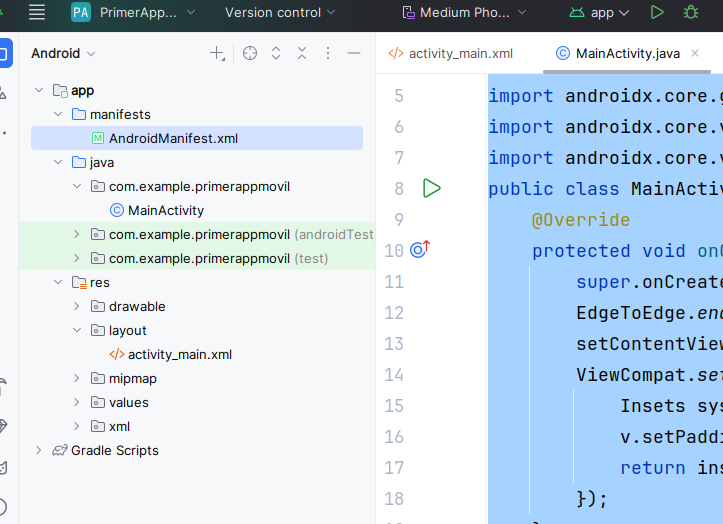
\includegraphics[width=0.95\linewidth]{00_Modificacion/PanelCarpetas2.png}    
\end{center}
\end{columns}   
\end{frame}


%\section{Agregar Codigo a la Interfaz}
\begin{frame}[fragile]
\frametitle{Agregar codigo a la interfaz}  


\begin{columns}

\column{0.30\linewidth}
\begin{itemize}
\item X
\end{itemize}

\column{0.70\linewidth}

\textit{Apariencia}
\begin{block}{Archivo \textbf{activity\_main.xml}}
\begin{minted}[linenos,fontsize=\tiny]{xml}
<?xml version="1.0" encoding="utf-8"?>
<androidx.constraintlayout.widget.ConstraintLayout 
    xmlns:android="http://schemas.android.com/apk/res/android"
    xmlns:app="http://schemas.android.com/apk/res-auto"
    xmlns:tools="http://schemas.android.com/tools"
    android:layout_width="match_parent"
    android:layout_height="match_parent"
    tools:context=".MainActivity">
    <TextView
        android:layout_width="wrap_content"
        android:layout_height="wrap_content"
        android:text="Hello World!"
        app:layout_constraintBottom_toBottomOf="parent"
        app:layout_constraintEnd_toEndOf="parent"
        app:layout_constraintStart_toStartOf="parent"
        app:layout_constraintTop_toTopOf="parent" />
</androidx.constraintlayout.widget.ConstraintLayout>
\end{minted}

\end{block}


\end{columns}
\end{frame}


%\section{Agregar Codigo a la Interfaz}
\begin{frame}[fragile]
\frametitle{Agregar codigo a la interfaz}  


\begin{columns}

\column{0.20\linewidth}
\begin{itemize}
\item X
\end{itemize}

\column{0.80\linewidth}
\textit{Comportamiento}
\begin{block}{Archivo \textbf{MainActivity.kt}}
\begin{minted}[linenos,fontsize=\tiny]{java}
package com.example.primerappmovil;
import android.os.Bundle;
import androidx.activity.EdgeToEdge;
import androidx.appcompat.app.AppCompatActivity;
import androidx.core.graphics.Insets;
import androidx.core.view.ViewCompat;
import androidx.core.view.WindowInsetsCompat;
public class MainActivity extends AppCompatActivity {
    @Override
    protected void onCreate(Bundle savedInstanceState) {
        super.onCreate(savedInstanceState);
        EdgeToEdge.enable(this);
        setContentView(R.layout.activity_main);
        ViewCompat.setOnApplyWindowInsetsListener(findViewById(R.id.main), (v, insets) -> {
            Insets systemBars = insets.getInsets(WindowInsetsCompat.Type.systemBars());
            v.setPadding(systemBars.left, systemBars.top, systemBars.right, systemBars.bottom);
            return insets;
        });
    }
}\end{minted}
\end{block}
\end{columns}
\end{frame}


\begin{frame}
\frametitle{Interfaz de Usuario}  

\begin{columns}

\column{0.60\linewidth}
\begin{itemize}
\item Define los controles de interfaz que la aplicacion muestra
\item Estos controles pueden estar agrupados en contenedores
\item El archivo \textbf{activity\_main.xml} es la definicion del layout (la organizacion de dichos componentes)
\end{itemize}

\begin{columns}
\column{0.50\linewidth}
\begin{center}
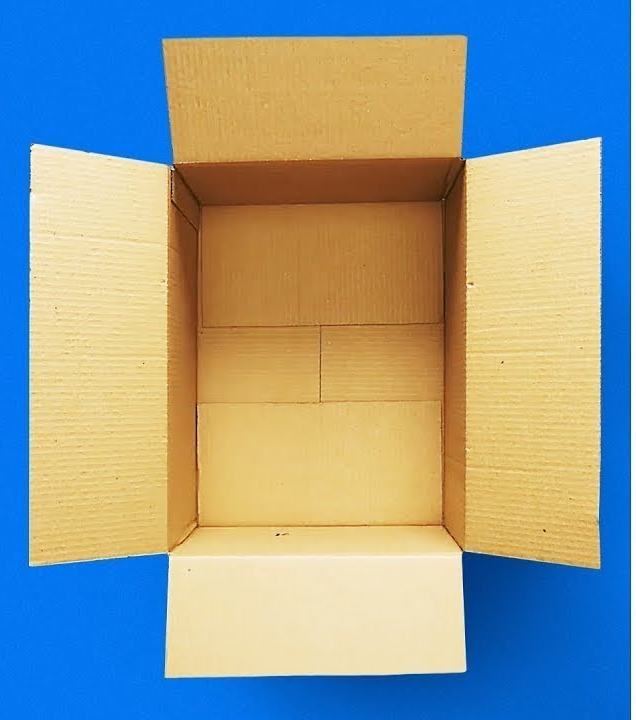
\includegraphics[width=0.75\linewidth]{00_Modificacion/CajaContenedora.png}    
\end{center}
\column{0.50\linewidth}
\begin{center}
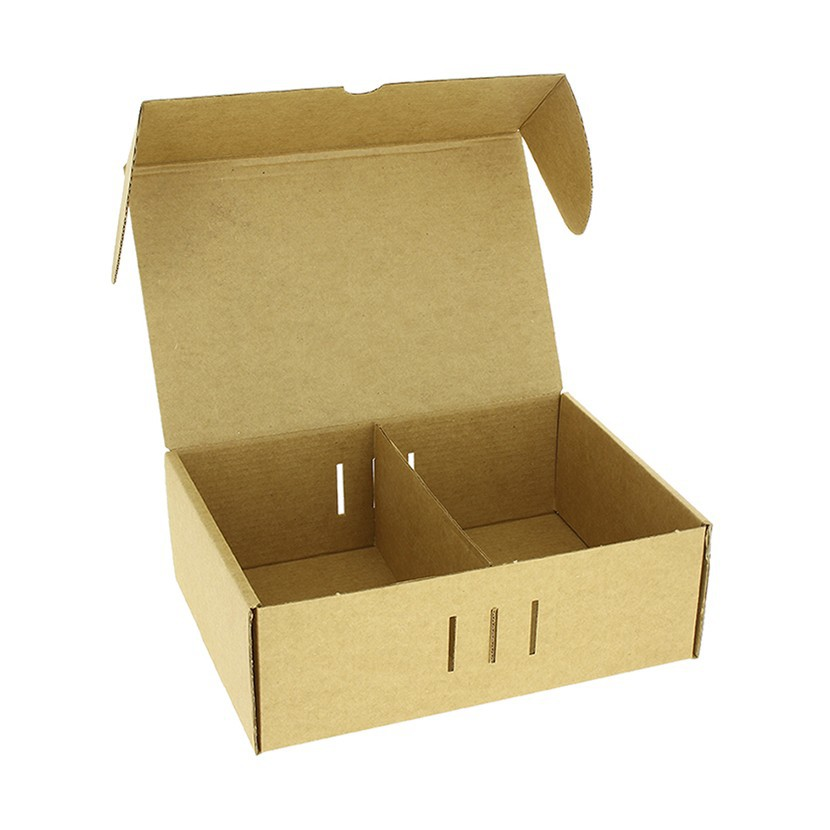
\includegraphics[width=0.75\linewidth]{00_Modificacion/Divisiones.jpg}    
\end{center}
\end{columns}

\column{0.40\linewidth}

\begin{center}
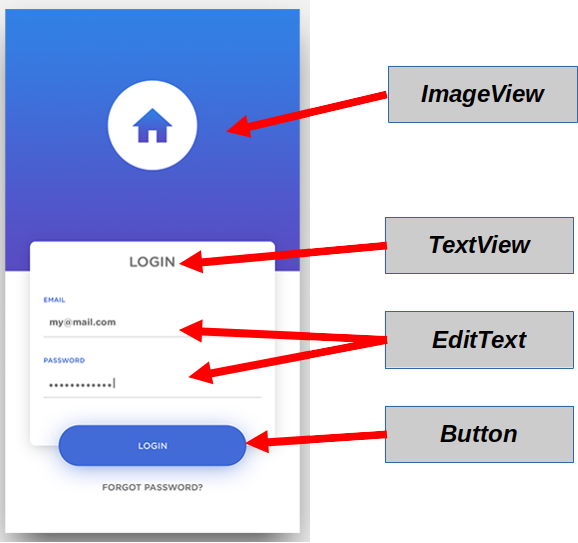
\includegraphics[width=0.95\linewidth]{00_Modificacion/ElementosInterfaz.png}    
\end{center}

\end{columns}

\end{frame}





\section{Demos}

\begin{frame}{Ejecucion de la Primer App en Android}
\begin{columns}
\begin{column}{0.8\textwidth}
\begin{itemize}
\item El dispositivo debe estar reconocido por Android y la compilación de la primera APP debe haber terminado. 
\item En la barra superior de Android Studio, presionar la flecha verde para instalar y ejecutar la app en el disposivito, 
\end{itemize}
\begin{block}{Demo \#00}
Muestra un TextView con el texto centrado "Hello World!"
\end{block}
\end{column}
\begin{column}{0.2\textwidth}
\begin{center}

 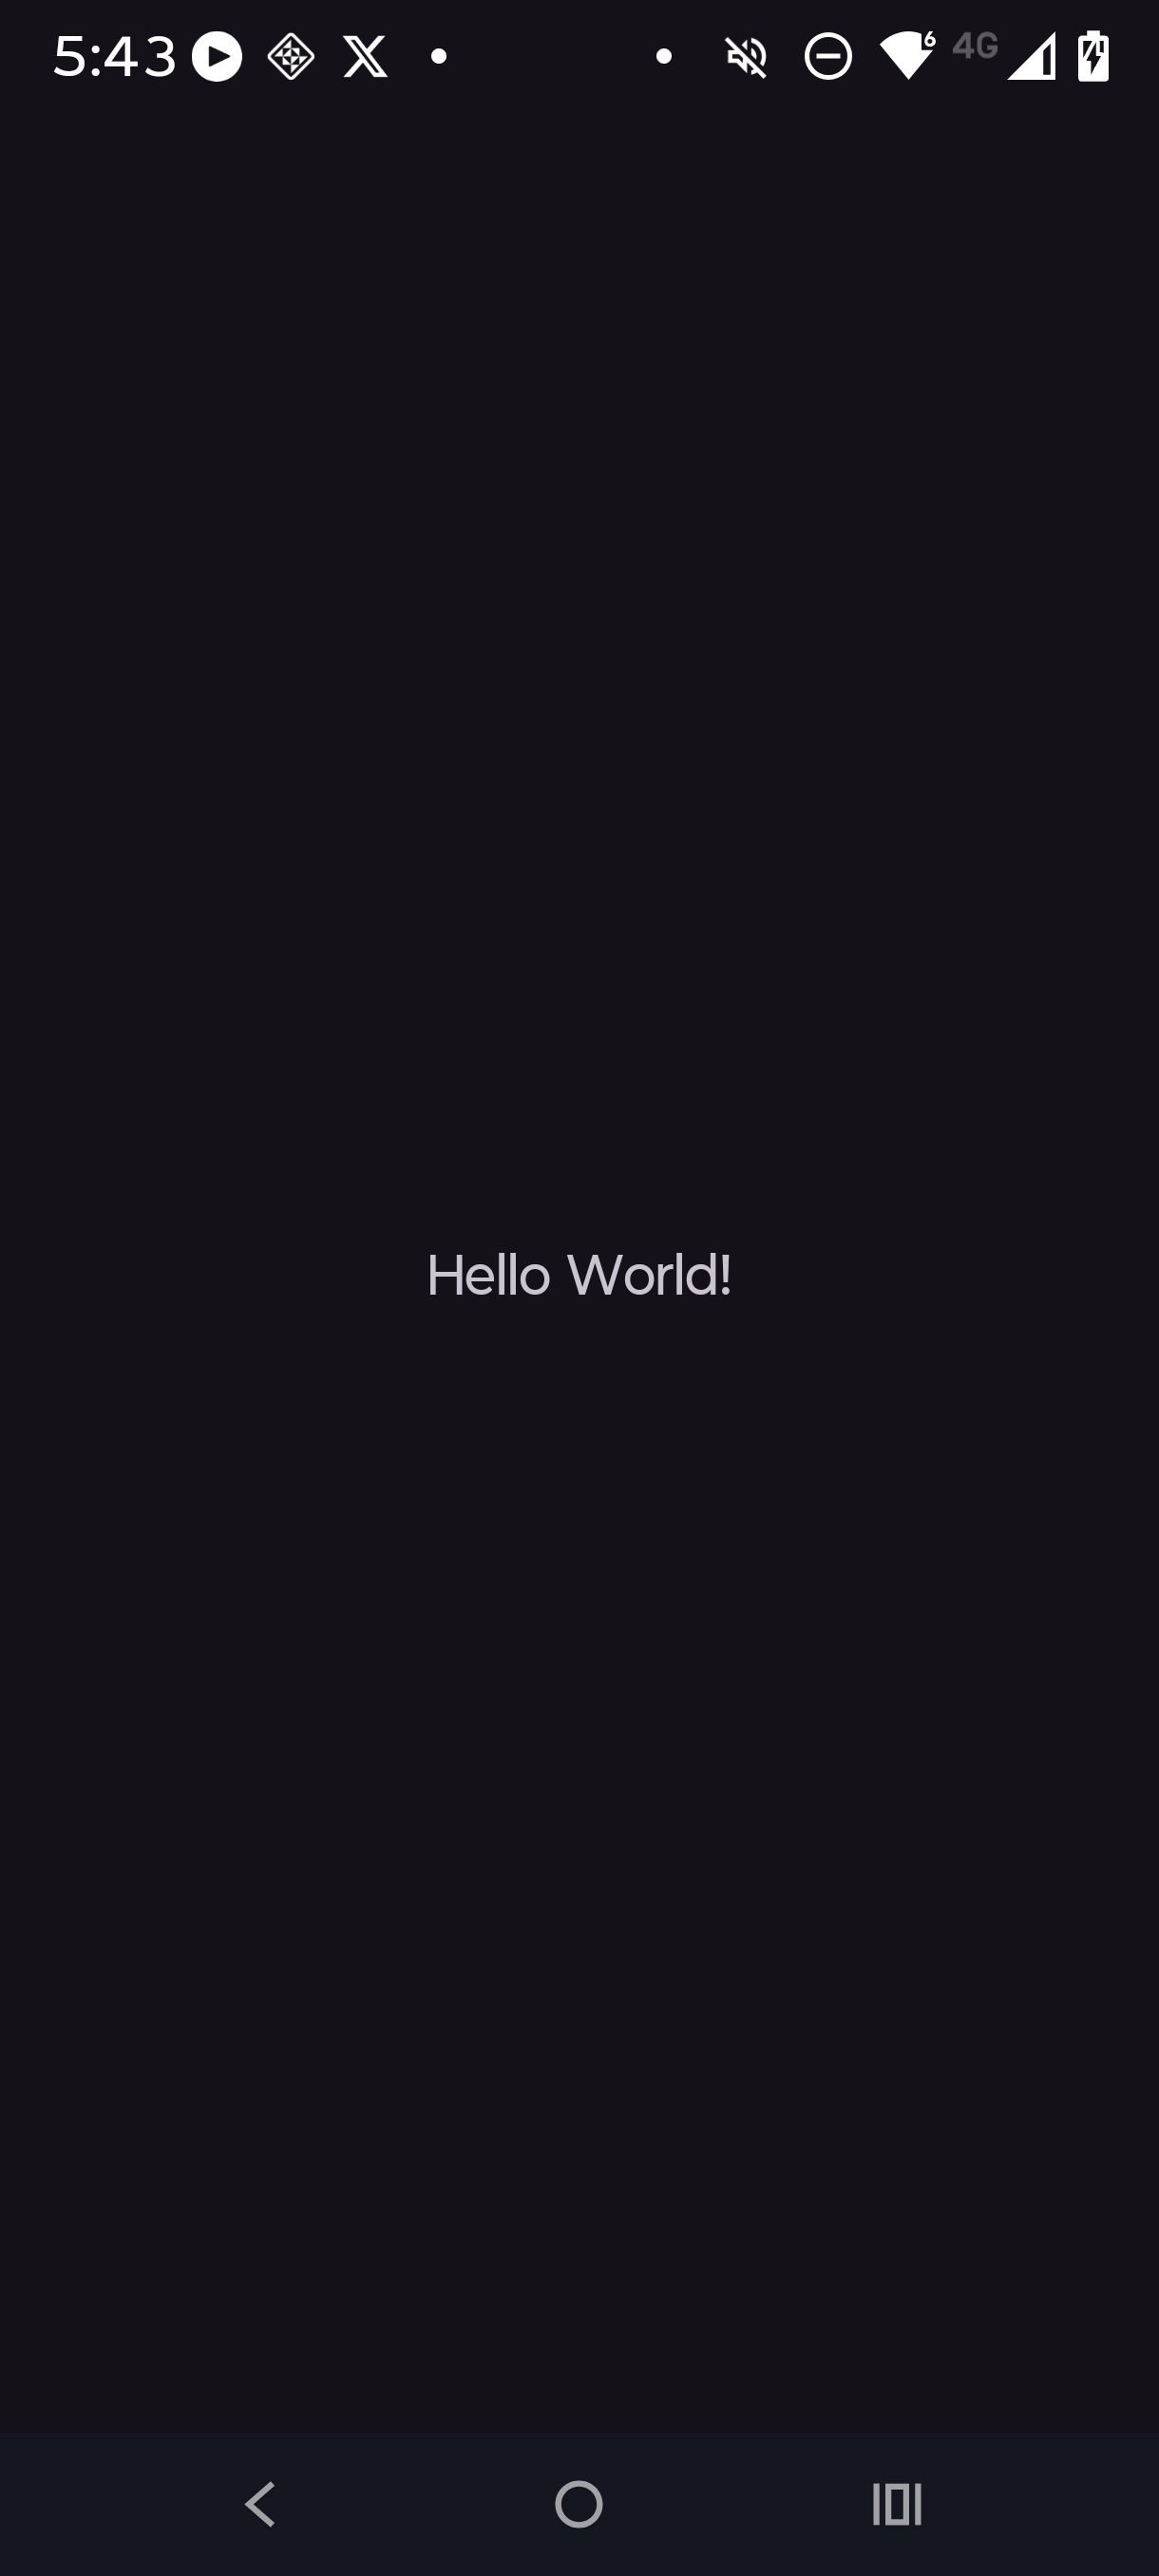
\includegraphics[width=0.98\textwidth]{02_TallerCBTis/figs/Demo00}
\end{center}
\end{column}
\end{columns}

\end{frame}


\begin{frame}[fragile]
\frametitle{Demo 01: Modificar el activity\_main.xml para aregar otro TextView}
\begin{columns}
\column{0.80\linewidth}
De los códigos fuentes en Github (como un archivo .zip), descomprimirlo y localizar los archivos mencionados a continuación:
\begin{itemize}
\item Copiar el archivo \textit{MainActivity\_Demo01.java} (dentro del Folder códigosJAVA) al mismo directorio donde esta el \textit{MainActivity.java}.
\item Copiar el archivo \textit{activity\_main\_demo01.xml} (dentro del Folder Carpeta\_layout) al mismo directorio donde esta el \textit{activity\_main.xml}
\item Modificar en el archivo AndroidManifest.xml la cadena \textit{.MainActivity} por \textit{.MainActivity\_Demo01}.
\end{itemize}

\begin{block}{Demo \#01}
Muestra un TextView con el texto centrado "Hello World!" (fuente verde, fondo rojo) 
\end{block}


\column{0.20\linewidth}

\begin{center}
 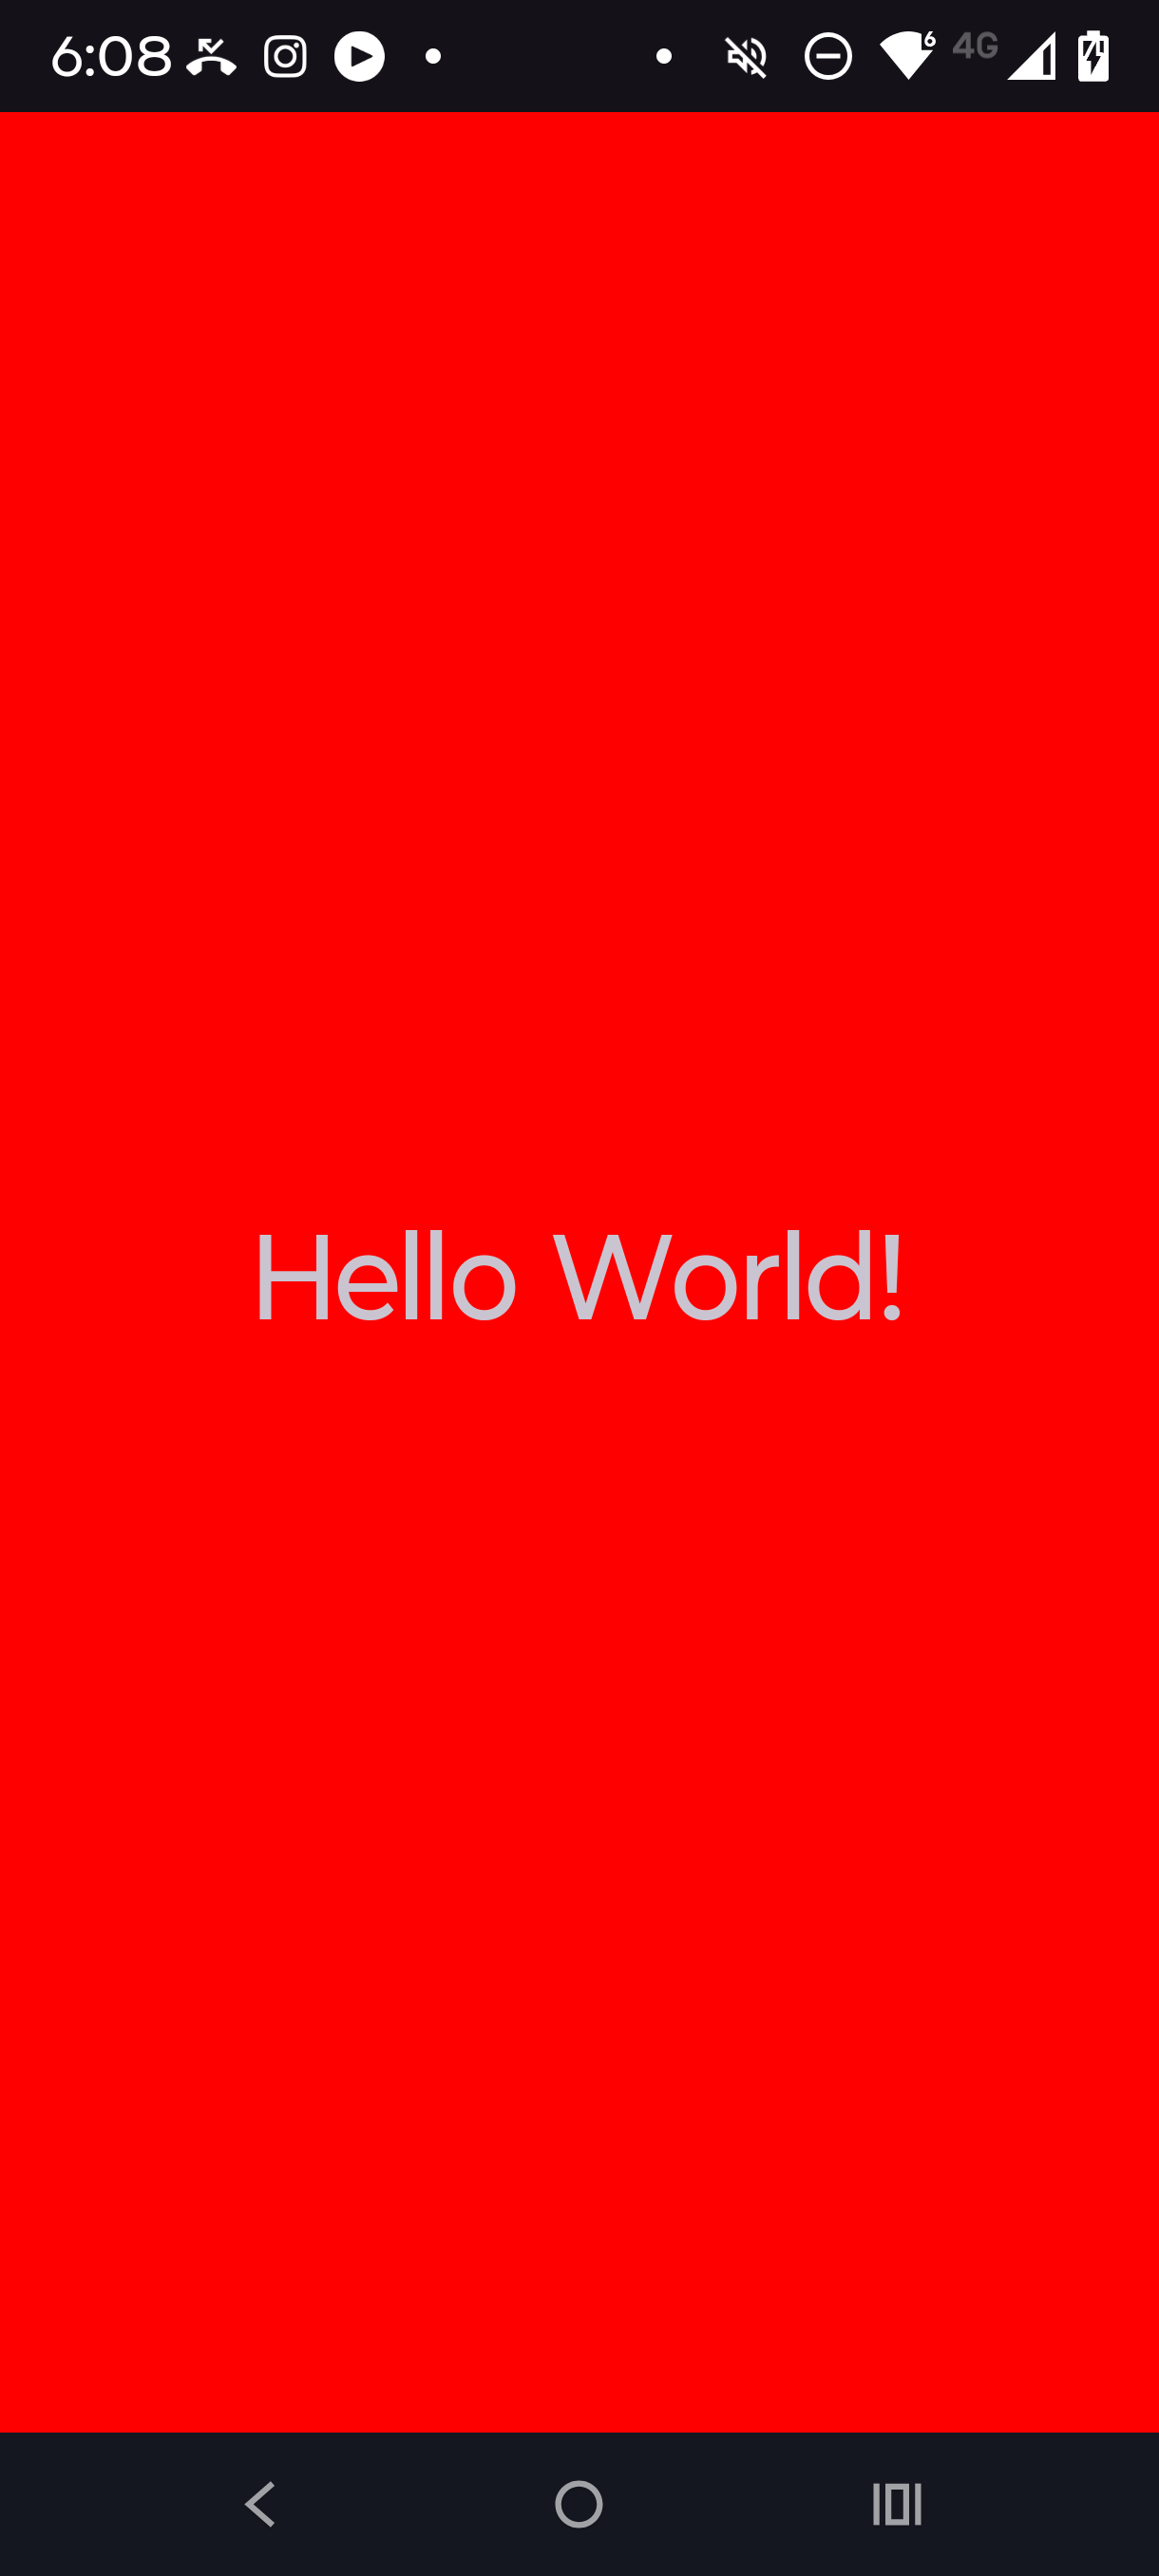
\includegraphics[width=0.98\textwidth]{02_TallerCBTis/figs/Demo01}
\end{center}

\end{columns}

\end{frame}


\begin{frame}{Modificaciones de Interés}

\begin{block}{Ejercicio \#01}
\begin{itemize}
\item Duplicar el TextView pero modificando el color de dichos componentes. 
\item Probar diferentes combinaciones del valor \textit{layout\_weight} en dichos componentes. 

\end{itemize}
\end{block}


\end{frame}



\begin{frame}{Componentes EditText y Button en Android}

\textbf{EditText: Campo de Entrada de Texto}
\begin{itemize}
    \item Permite al usuario introducir y editar texto dentro de la aplicación.
    \item Se utiliza en formularios, búsquedas y captura de datos.
    \item Soporta distintos tipos de entrada (texto, número, correo, contraseña).
    \item Puede configurarse mediante atributos XML o código Java/Kotlin.
\end{itemize}

\vspace{0.4cm}

\textbf{Button: Botón de Interacción}
\begin{itemize}
    \item Es un componente que permite al usuario ejecutar acciones al hacer clic.
    \item Se utiliza para enviar datos, navegar entre pantallas o activar eventos.
    \item Puede personalizarse en texto, color, tamaño y estilo.
\end{itemize}


\end{frame}



\begin{frame}[fragile]
\frametitle{Demo 02: Agregar un EditText y un Button}
\begin{columns}
\column{0.80\linewidth}
De los códigos fuentes en Github (como un archivo .zip), descomprimirlo y localizar los archivos mencionados a continuación:
\begin{itemize}
\item Copiar el archivo \textit{MainActivity\_Demo02.java} (dentro del Folder códigosJAVA) al mismo directorio donde esta el \textit{MainActivity.java}.
\item Copiar el archivo \textit{activity\_main\_demo02.xml} (dentro del Folder Carpeta\_layout) al mismo directorio donde esta el \textit{activity\_main.xml}.
\item Modificar en el archivo \textit{AndroidManifest.xml} la cadena \textit{..MainActivity\_Demo01} por \textit{.MainActivity\_Demo02}
\end{itemize}

\begin{block}{Demo \#02}
Muestra una App con dos TextViews, un EditText y un Botton. Cuando el usuario ingresa un dato y presiona le boton aparece un mensaje con el dato ingresado 
\end{block}


\column{0.20\linewidth}

\begin{center}
 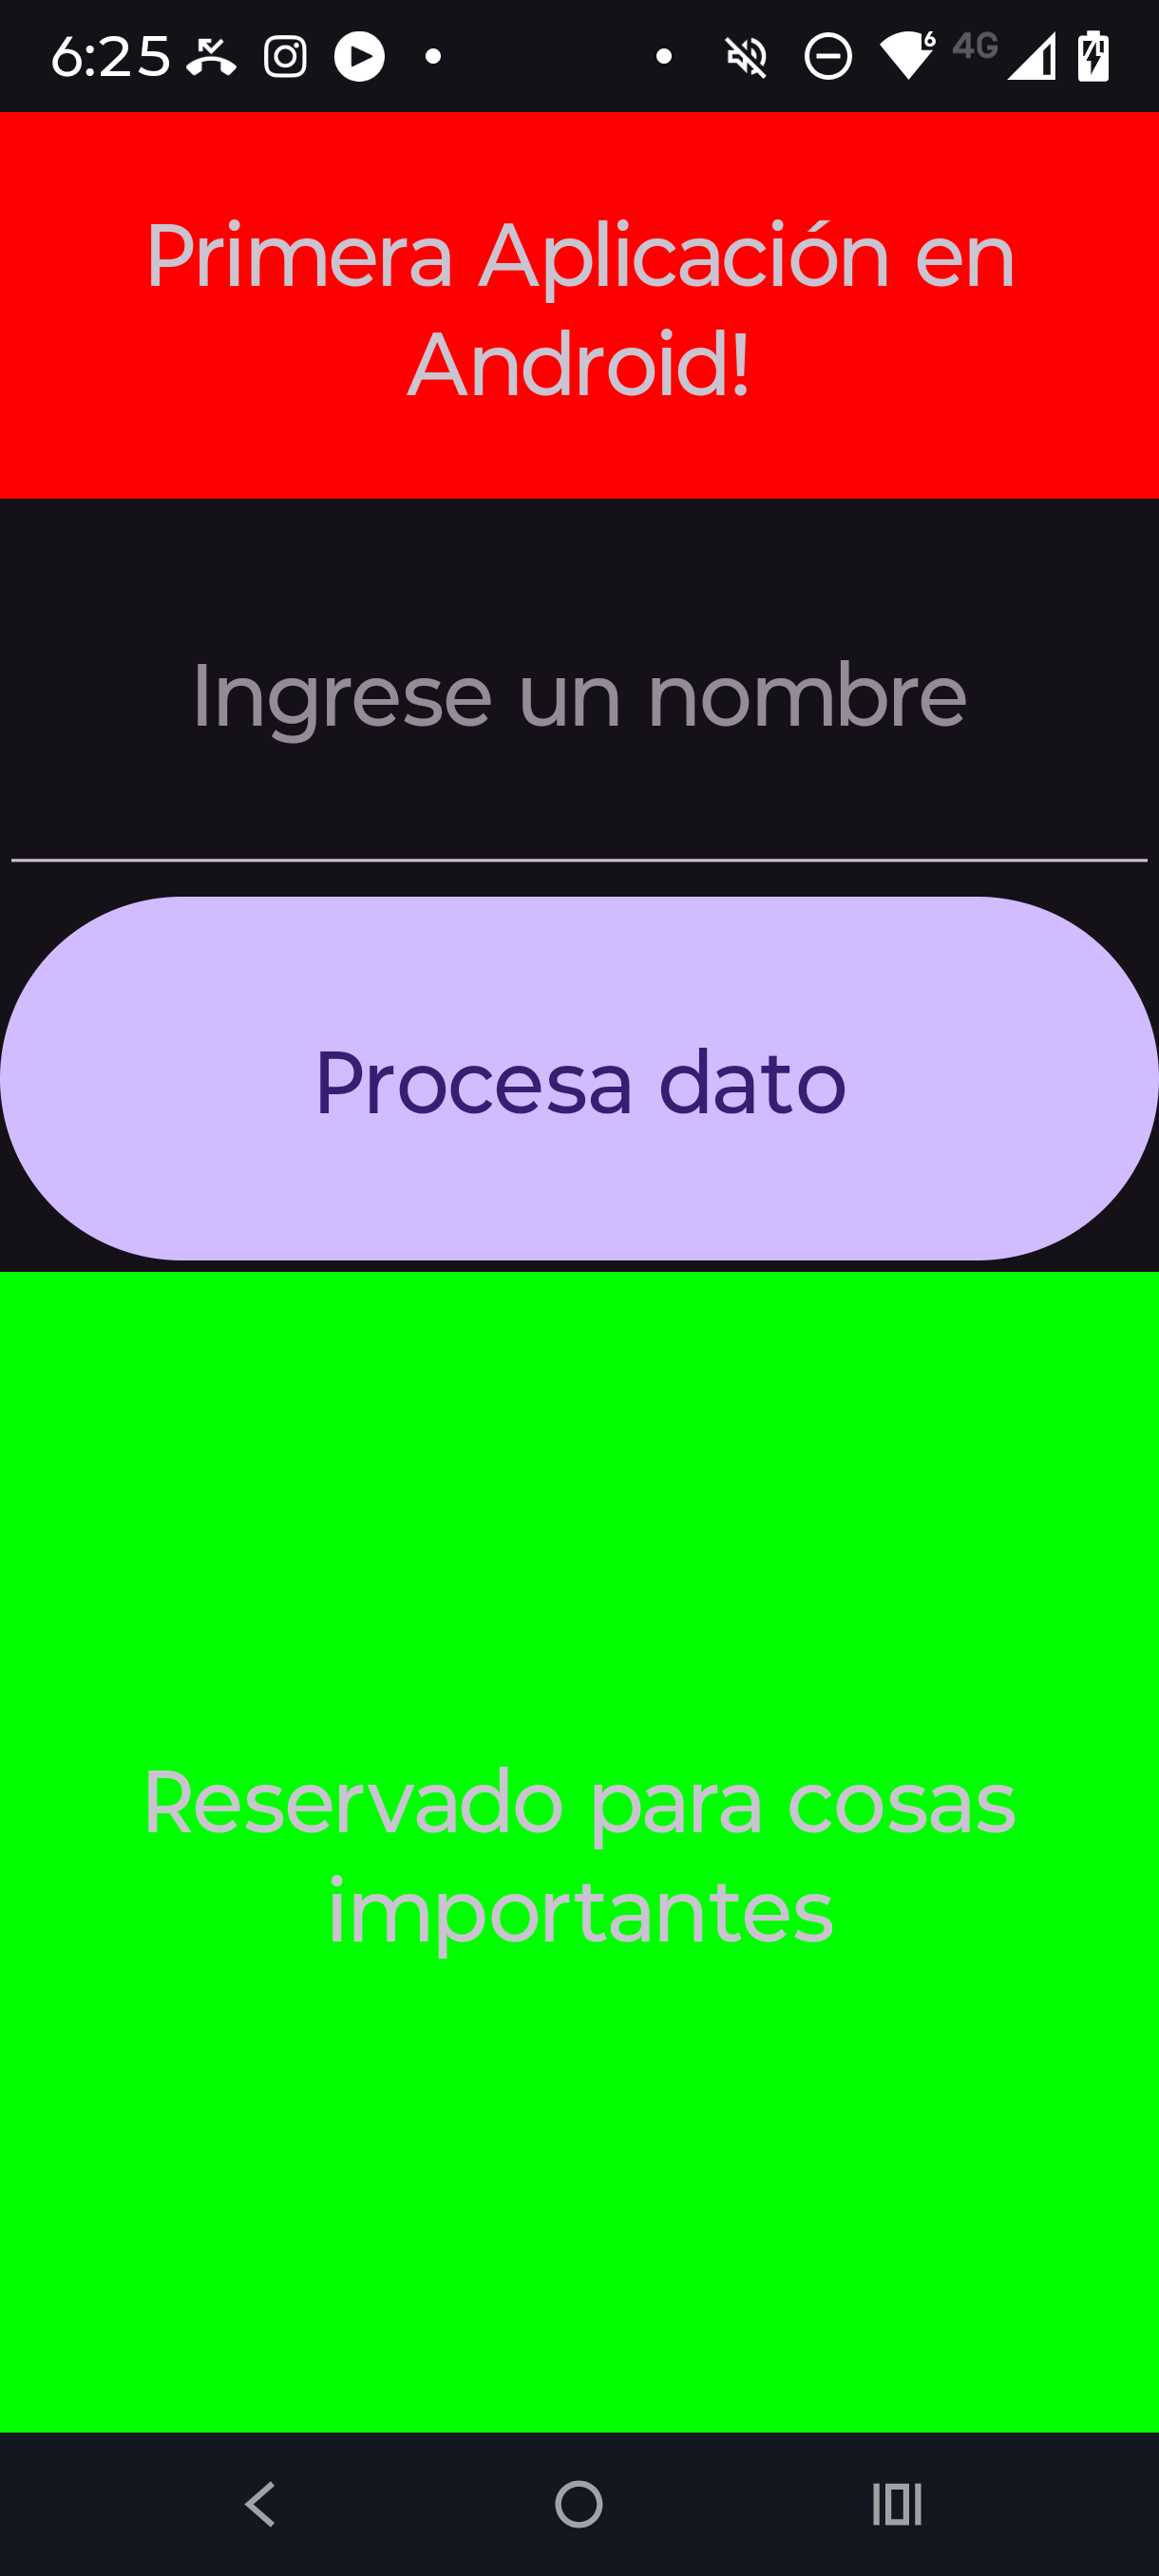
\includegraphics[width=0.98\textwidth]{02_TallerCBTis/figs/Demo02}
\end{center}

\end{columns}

\end{frame}




\begin{frame}{Uso de GridLayout en Android}
\textbf{¿Qué es GridLayout?}

\begin{itemize}
    \item Es un contenedor de diseño (ViewGroup) que organiza los elementos en una cuadrícula de filas y columnas.
    \item Permite ubicar componentes de manera estructurada y alineada.
\end{itemize}

\vspace{0.4cm}

\textbf{¿Para qué sirve?}
\begin{itemize}
    \item Diseñar interfaces organizadas en forma de tabla.
    \item Alinear múltiples elementos (botones, imágenes, textos) fácilmente.
    \item Crear interfaces dinámicas como teclados, galerías o tableros de juego.
\end{itemize}

\vspace{0.4cm}

\textbf{Características principales:}
\begin{itemize}
    \item Define número de filas y columnas.
    \item Permite que los elementos ocupen múltiples celdas (rowSpan, columnSpan).
    \item Soporta alineación y distribución del espacio.
\end{itemize}


\end{frame}


\begin{frame}[fragile]
\frametitle{Demo 03: Agregar un Panel de Botones utilizando un GridLayout}
\begin{columns}
\column{0.80\linewidth}
Del Repositorio Github:
\begin{itemize}
\item Copiar el archivo MainActivity\_Demo03.java (dentro del Folder códigosJAVA) al mismo directorio donde esta el MainActivity.java
\item Copiar el archivo activity\_main\_demo03.xml (dentro del Folder Carpeta\_layout) al mismo directorio donde esta el activity\_main.xml
\item Modificar en el archivo AndroidManifest.xml la cadena \textit{.MainActivity\_Demo02} por \textit{.MainActivity\_Demo03}
\end{itemize}

\begin{block}{Demo \#03}
Muestra una App con un panel de botones, que muestra un Toast para cada boton presionado por el usuario.  
\end{block}


\column{0.20\linewidth}

\begin{center}
 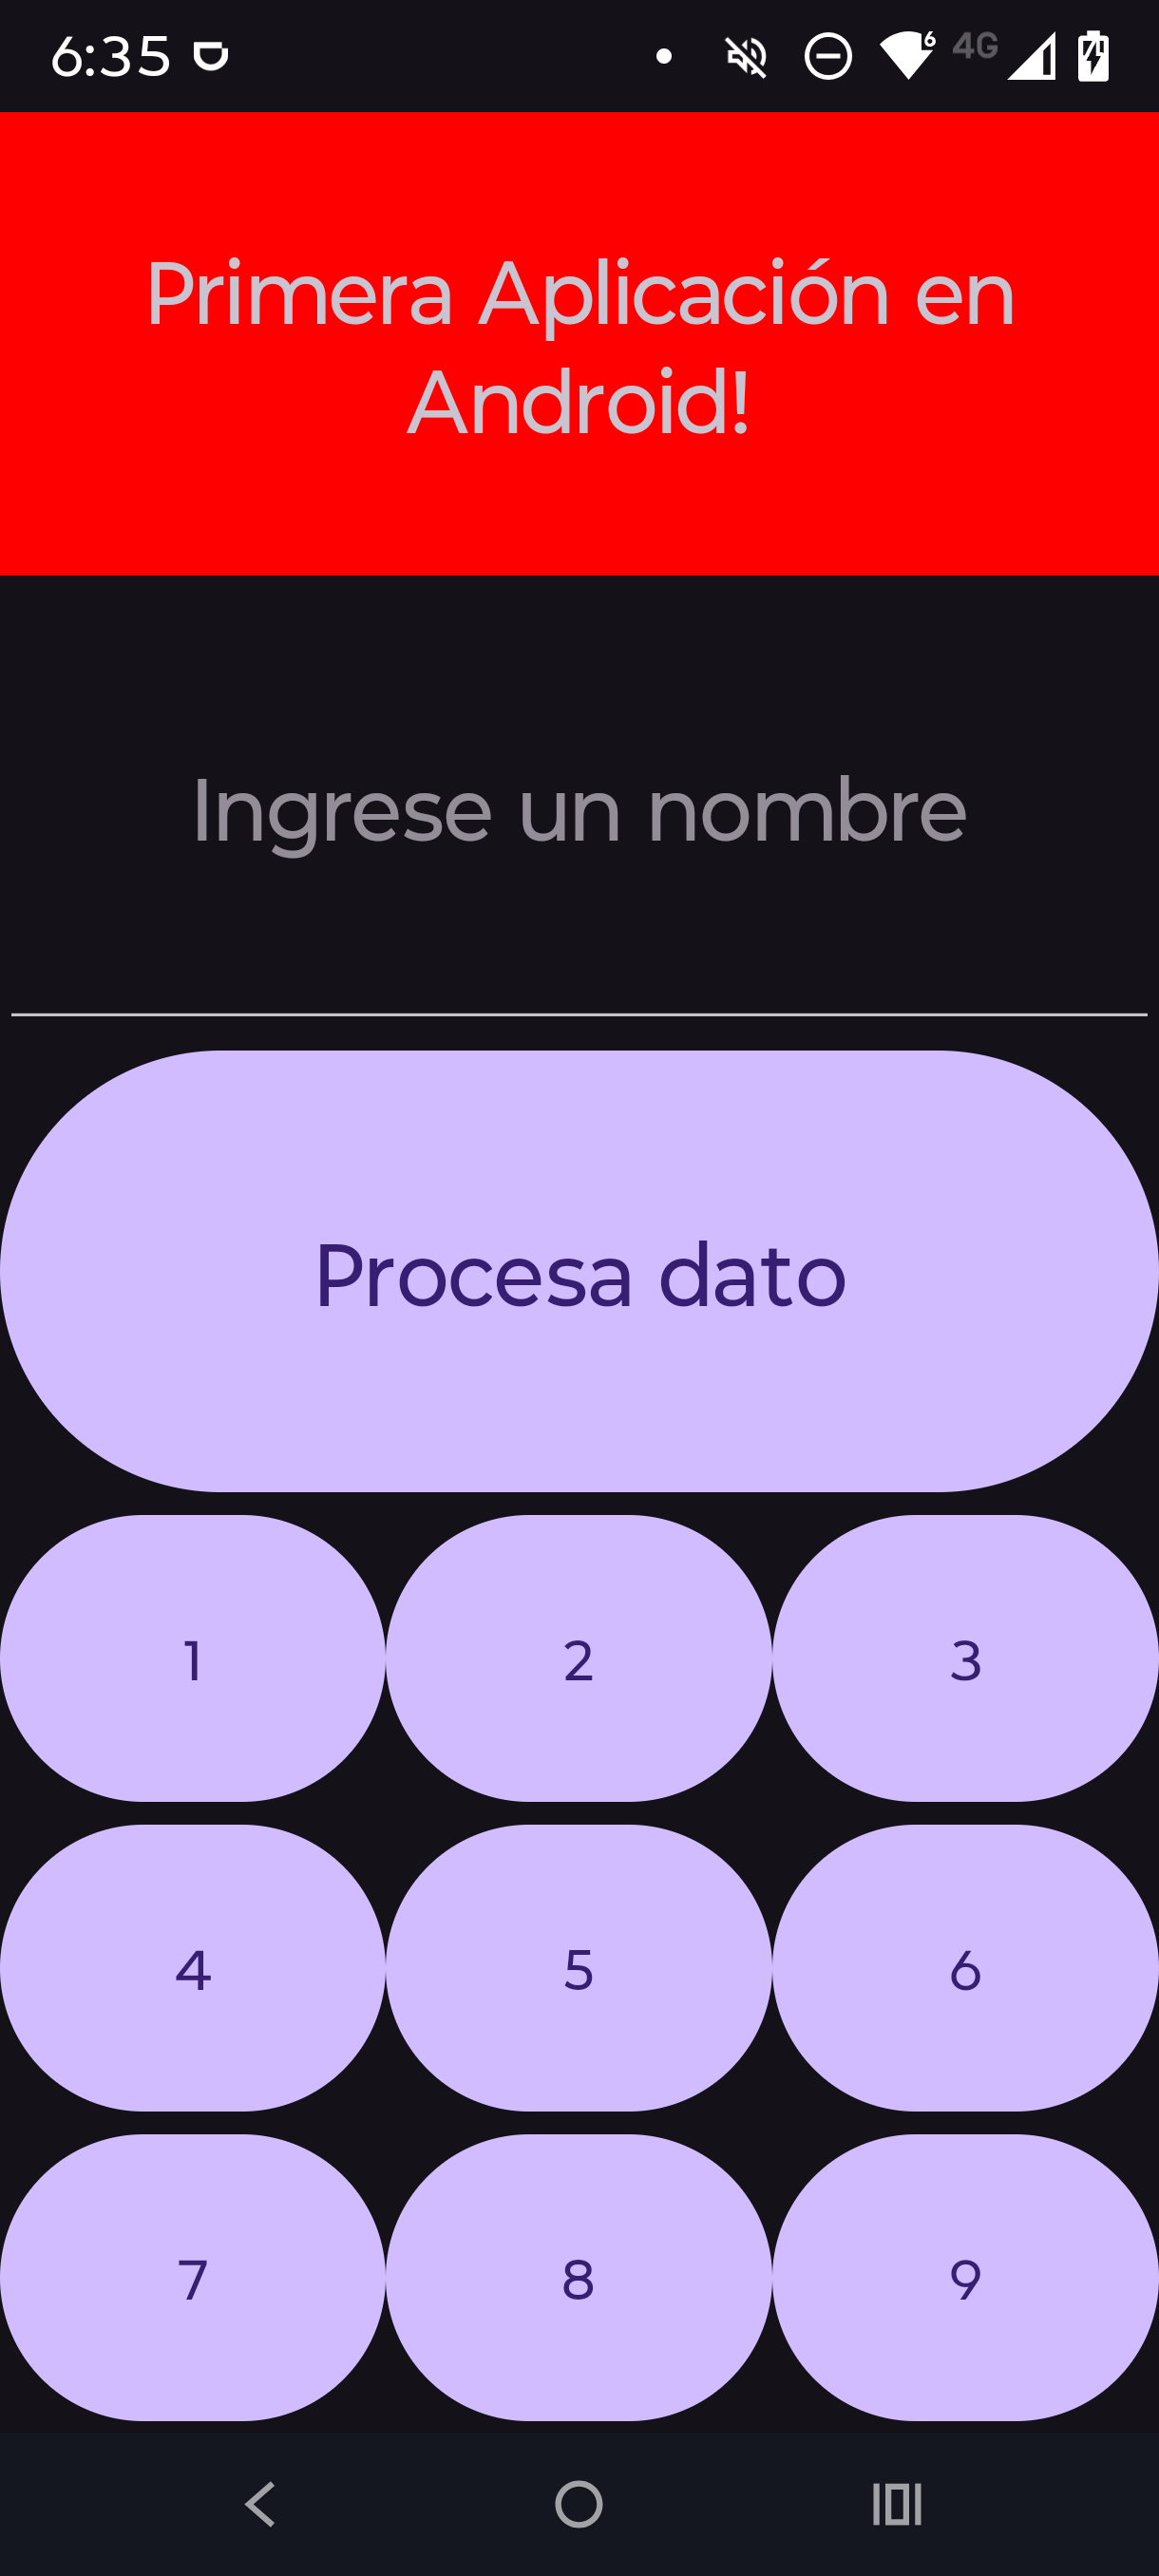
\includegraphics[width=0.98\textwidth]{02_TallerCBTis/figs/Demo03}
\end{center}

\end{columns}

\end{frame}





\begin{frame}{Componentes CheckBox e ImageView en Android}

\textbf{CheckBox: ¿Para qué sirve?}
\begin{itemize}
    \item Permite al usuario seleccionar una o múltiples opciones de una lista.
    \item Cada opción es independiente (no excluyente).
    \item Es útil en formularios, configuraciones o encuestas.
\end{itemize}

\vspace{0.4cm}

\textbf{Características del CheckBox:}
\begin{itemize}
    \item Puede estar en estado seleccionado o no seleccionado.
    \item Permite manejar eventos de cambio (OnCheckedChangeListener).
\end{itemize}

\vspace{0.4cm}

\textbf{ImageView: ¿Para qué sirve?}
\begin{itemize}
    \item Se utiliza para mostrar imágenes en la interfaz de usuario.
    \item Soporta recursos locales (drawable) o imágenes desde URL.
\end{itemize}

\vspace{0.4cm}

\textbf{Características del ImageView:}
\begin{itemize}
    \item Permite escalar, ajustar y posicionar imágenes.
    \item Compatible con diferentes formatos (PNG, JPG, SVG - mediante librerías).
\end{itemize}


\end{frame}


\begin{frame}[fragile]
\frametitle{Demo 04: Agregar un CheckBox y un ImageView}
\begin{columns}
\column{0.80\linewidth}
Del Repositorio Github:
\begin{itemize}
\item Copiar el archivo MainActivity\_Demo04.java (dentro del Folder códigosJAVA) al mismo directorio donde esta el MainActivity.java
\item Copiar el archivo activity\_main\_demo04.xml (dentro del Folder Carpeta\_layout) al mismo directorio donde esta el activity\_main.xml
\item Copiar el archivo \textit{upv.png} dentro de la folder \textit{Carpeta\_drawable} en el directorio \textit{res/drawable} del proyecto de AS.


\item Modificar en el archivo AndroidManifest.xml la cadena \textit{.MainActivity\_Demo03} por \textit{.MainActivity\_Demo04}
\end{itemize}

\begin{block}{Demo \#04}
Una App con in Checkbox y un ImageView. Al modificar el estado del CheckBox, el texto de un Textview cambia. Al presionar el primer boton, un Toast muestra el estado del Checkbox.  
\end{block}


\column{0.20\linewidth}

\begin{center}
 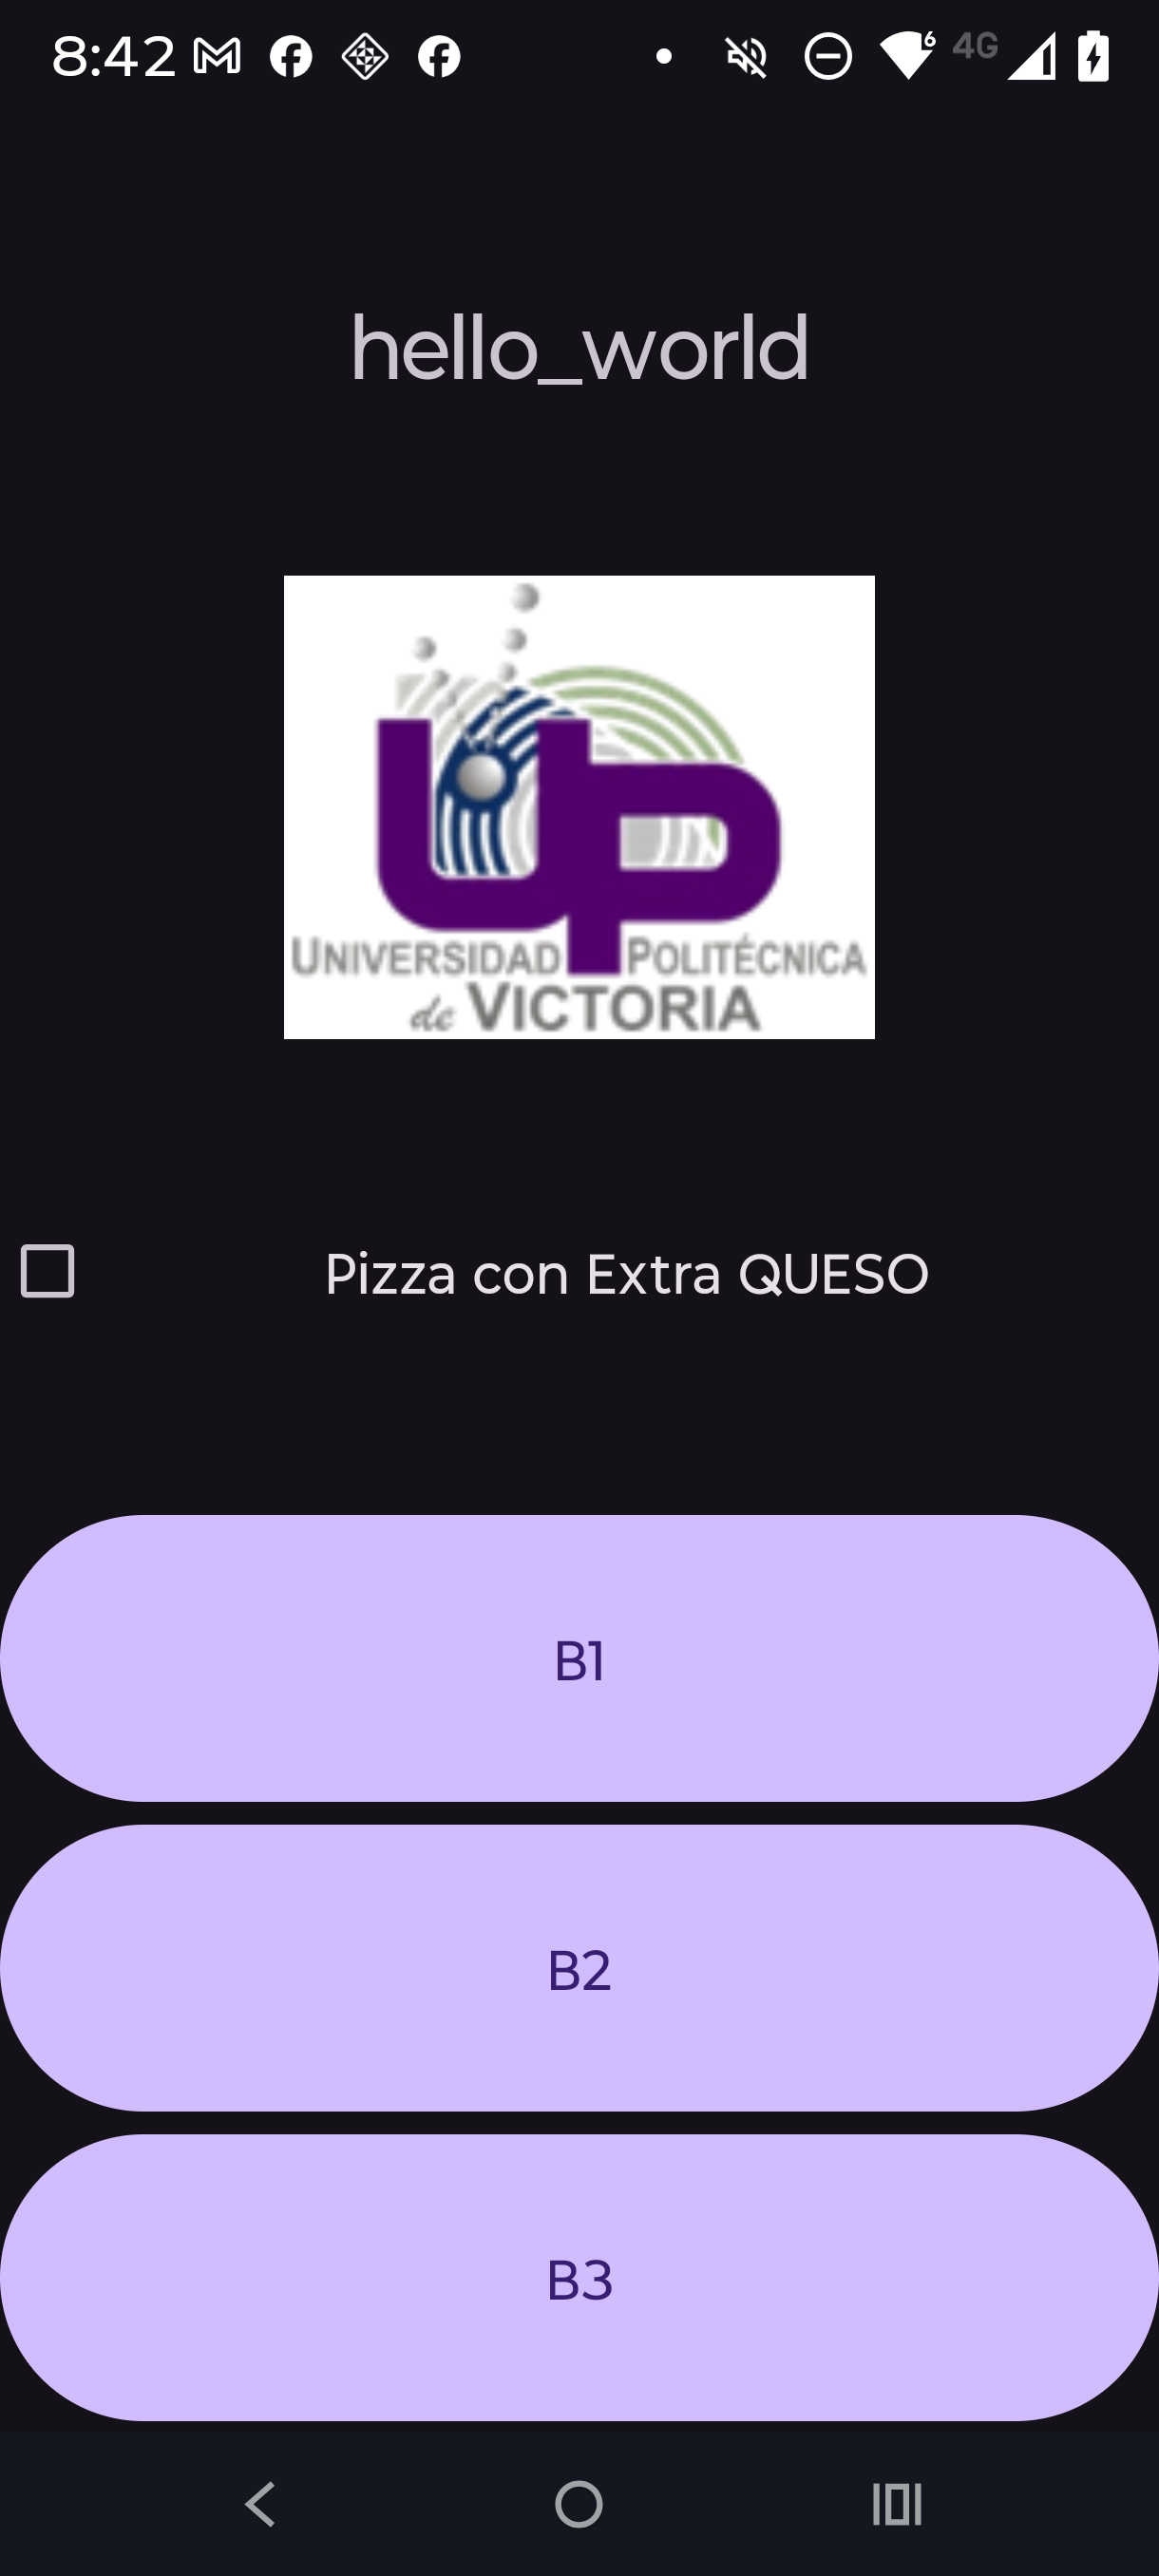
\includegraphics[width=0.98\textwidth]{02_TallerCBTis/figs/Demo04}
\end{center}

\end{columns}

\end{frame}




\begin{frame}[fragile]
\frametitle{Demo 05: Agregar un RadioGroup}
\begin{columns}
\column{0.80\linewidth}
Del Repositorio Github:
\begin{itemize}
\item Copiar el archivo MainActivity\_Demo05.java (dentro del Folder códigosJAVA) al mismo directorio donde esta el MainActivity.java
\item Copiar el archivo activity\_main\_demo05.xml (dentro del Folder Carpeta\_layout) al mismo directorio donde esta el activity\_main.xml
\item Copiar los archivos \textit{cgup.jpg} y \textit{logo\_upv\_2019.png} localizados dentro de la folder \textit{Carpeta\_drawable} en el directorio \textit{res/drawable} del proyecto de AS.
\item Modificar en el archivo AndroidManifest.xml la cadena \textit{.MainActivity\_Demo04} por \textit{.MainActivity\_Demo05}
\end{itemize}

\begin{block}{Demo \#05}
Muestra una App con un RadioGroup. El ImageView cambia basado en la seleccion del usuario.    
\end{block}


\column{0.20\linewidth}

\begin{center}
 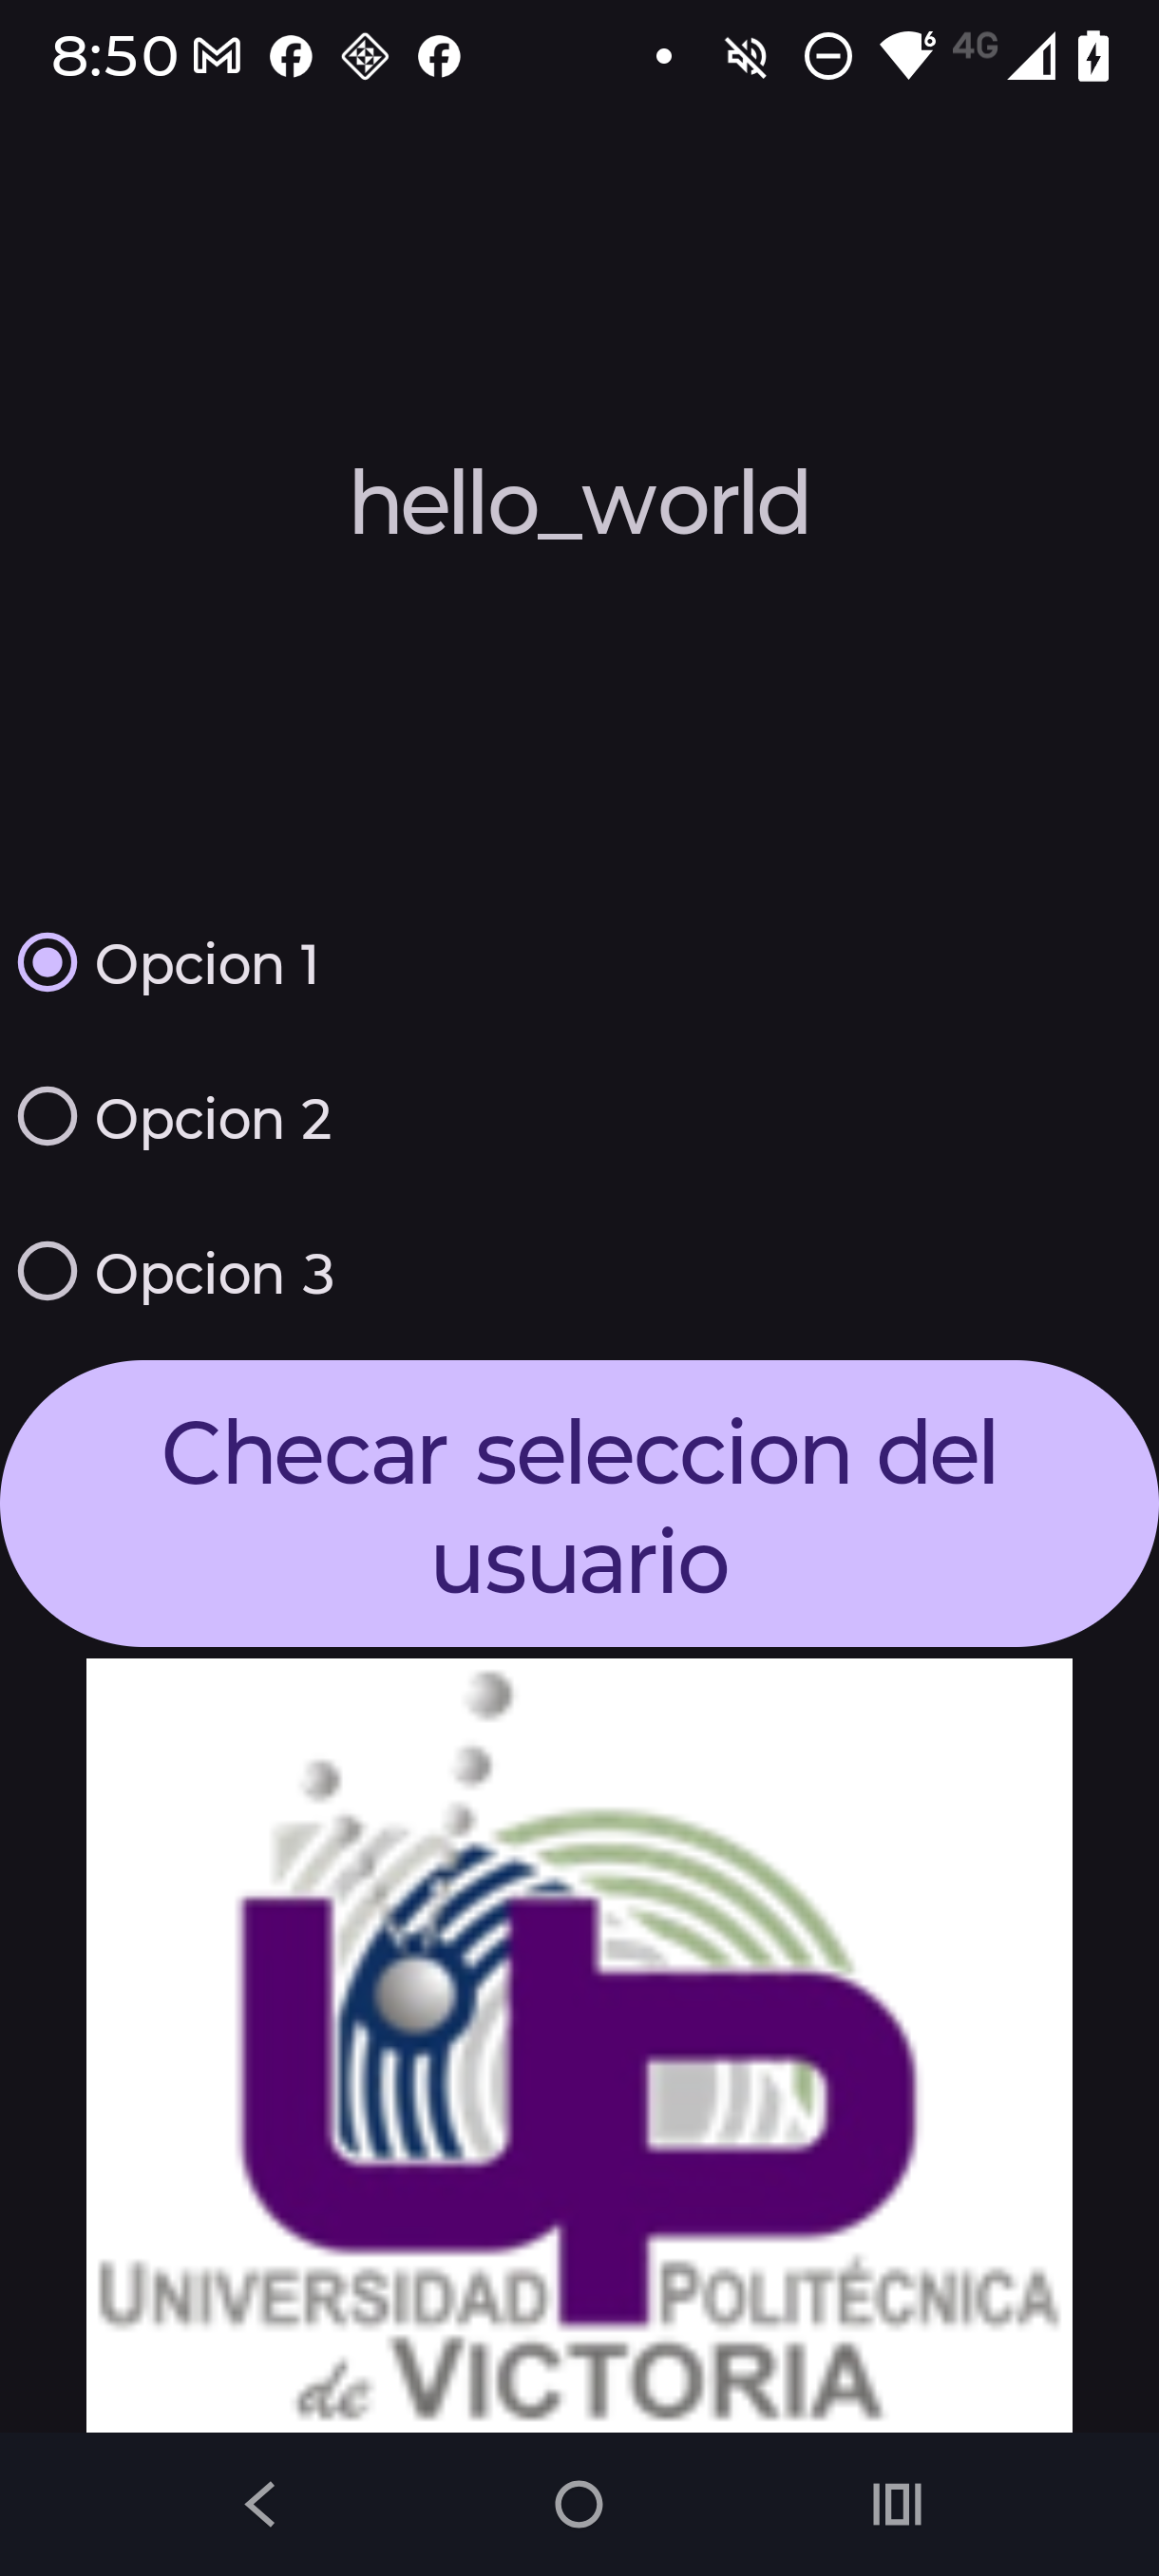
\includegraphics[width=0.98\textwidth]{02_TallerCBTis/figs/Demo05}
\end{center}

\end{columns}

\end{frame}



\begin{frame}{Componentes Adapter y ListView en Android}
\textbf{¿Qué es ListView?}

\begin{itemize}
    \item Es un componente de interfaz que permite mostrar una lista desplazable de elementos.
    \item Cada elemento puede contener texto, imágenes u otros componentes.
    \item Es útil para mostrar datos en forma de lista vertical.
\end{itemize}

\vspace{0.4cm}

\textbf{¿Qué es un Adapter?}

\begin{itemize}
    \item Es un intermediario entre los datos y el ListView.
    \item Se encarga de convertir los datos (arreglos, listas, bases de datos) en vistas visuales.
    \item Permite personalizar cómo se muestra cada elemento de la lista.
\end{itemize}

\vspace{0.4cm}

\textbf{Relación entre Adapter y ListView:}
\begin{itemize}
    \item El ListView solicita los datos al Adapter.
    \item El Adapter genera la vista de cada elemento.
\end{itemize}


\end{frame}



\begin{frame}{Componentes Adapter y ListView en Android}
\textbf{¿Qué es ListView?}

\begin{itemize}
    \item Es un componente de interfaz que permite mostrar una lista desplazable de elementos.
    \item Cada elemento puede contener texto, imágenes u otros componentes.
    \item Es útil para mostrar datos en forma de lista vertical.
\end{itemize}

\vspace{0.4cm}

\textbf{¿Qué es un Adapter?}

\begin{itemize}
    \item Es un intermediario entre los datos y el ListView.
    \item Se encarga de convertir los datos (arreglos, listas, bases de datos) en vistas visuales.
    \item Permite personalizar cómo se muestra cada elemento de la lista.
\end{itemize}

\vspace{0.4cm}

\textbf{Relación entre Adapter y ListView:}
\begin{itemize}
    \item El ListView solicita los datos al Adapter.
    \item El Adapter genera la vista de cada elemento.
\end{itemize}


\end{frame}



\begin{frame}[fragile]
\frametitle{Demo 06: Agregar un ListView}
\begin{columns}
\column{0.80\linewidth}
Del Repositorio Github:
\begin{itemize}
\item Copiar el archivo MainActivity\_Demo06.java (dentro del Folder códigosJAVA) al mismo directorio donde esta el MainActivity.java
\item Copiar el archivo activity\_main\_demo06.xml (dentro del Folder Carpeta\_layout) al mismo directorio donde esta el activity\_main.xml
%\item Copiar los archivos \textit{cgup.jpg} y \textit{logo\_upv\_2019.png} localizados dentro de la folder \textit{Carpeta\_drawable} en el directorio \textit{res/drawable} del proyecto de AS.
\item Modificar en el archivo AndroidManifest.xml la cadena \textit{.MainActivity\_Demo05} por \textit{.MainActivity\_Demo06}
\end{itemize}

\begin{block}{Demo \#06}
Muestra una App con un ListView. El usuario agregar elementos al presionar el boton superior.    
\end{block}


\column{0.20\linewidth}

\begin{center}
 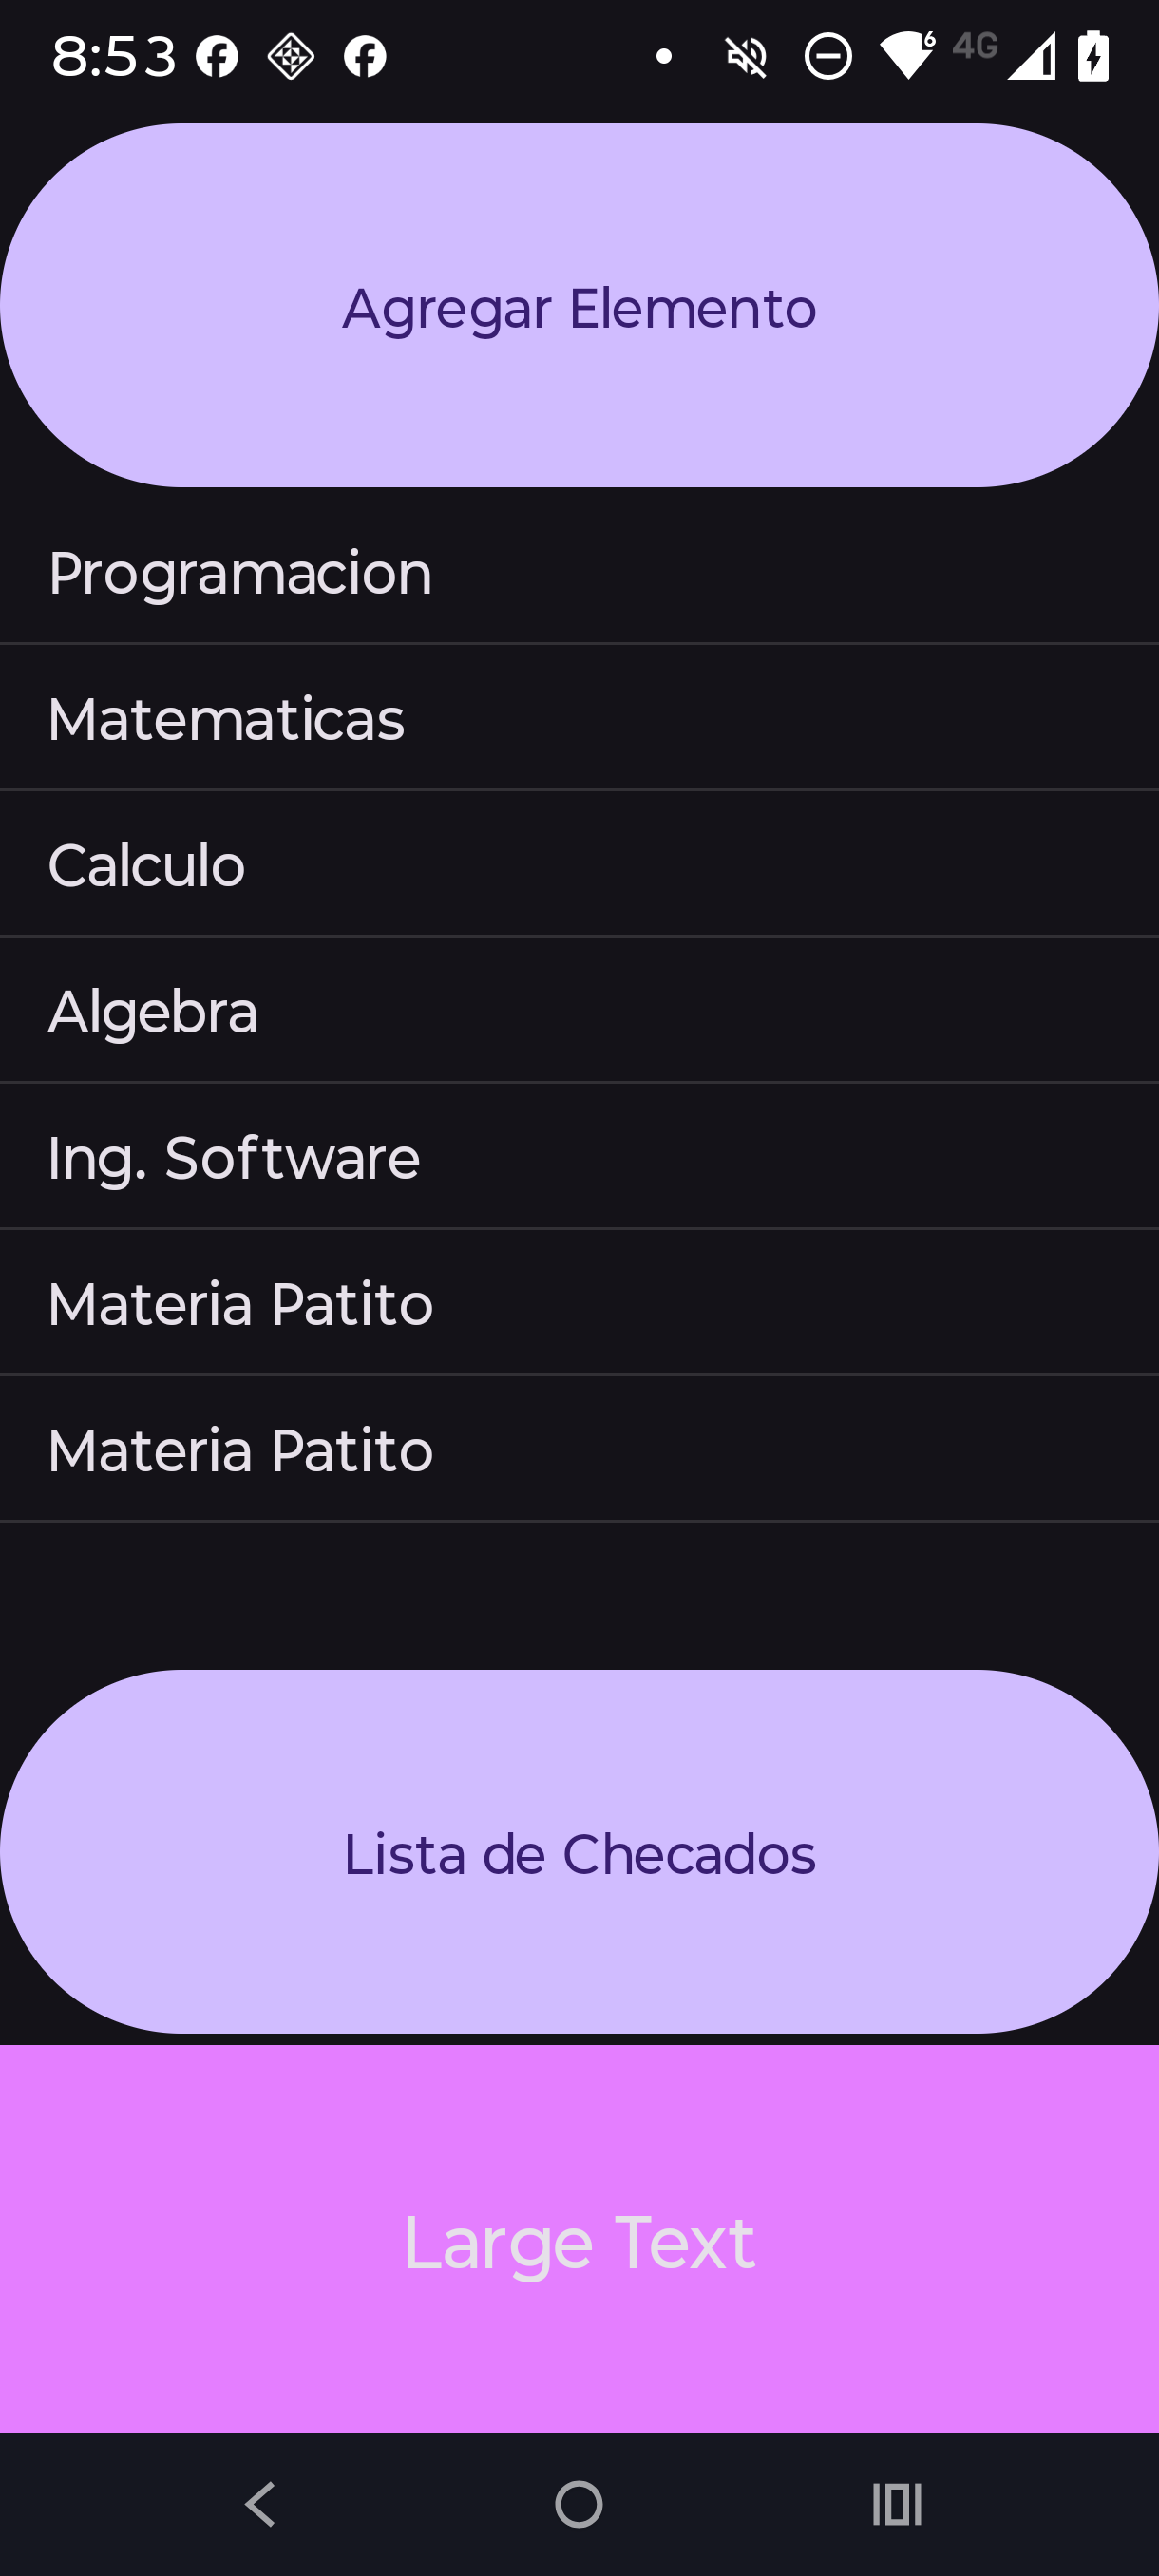
\includegraphics[width=0.98\textwidth]{02_TallerCBTis/figs/Demo06}
\end{center}

\end{columns}

\end{frame}



\begin{frame}{Spinner vs ListView en Android}
\textbf{¿Qué es un Spinner?}

\begin{itemize}
    \item Es un componente que permite seleccionar una opción de una lista desplegable.
    \item Ocupa poco espacio en pantalla.
    \item Ideal cuando se requiere elegir una sola opción entre varias.
\end{itemize}

\vspace{0.4cm}

\textbf{¿Qué es un ListView?}

\begin{itemize}
    \item Es un componente que muestra una lista de elementos visibles en pantalla.
    \item Permite visualizar múltiples opciones al mismo tiempo.
    \item Puede soportar selección simple o múltiple.
\end{itemize}

\vspace{0.4cm}

\textbf{Diferencias principales:}

\begin{itemize}
    \item \textbf{Espacio:} Spinner es compacto, ListView requiere más espacio.
    \item \textbf{Interacción:} Spinner usa menú desplegable, ListView muestra lista directa.
    \item \textbf{Uso:} Spinner para selección rápida; ListView para exploración de datos.
    \item \textbf{Cantidad de datos:} ListView es más adecuado para listas largas.
\end{itemize}

\end{frame}



\begin{frame}[fragile]
\frametitle{Demo 07: Agregar un Spinner}
\begin{columns}
\column{0.80\linewidth}
Del Repositorio Github:
\begin{itemize}
\item Copiar el archivo MainActivity\_Demo07.java (dentro del Folder códigosJAVA) al mismo directorio donde esta el MainActivity.java
\item Copiar el archivo activity\_main\_demo07.xml (dentro del Folder Carpeta\_layout) al mismo directorio donde esta el activity\_main.xml
%\item Copiar los archivos \textit{cgup.jpg} y \textit{logo\_upv\_2019.png} localizados dentro de la folder \textit{Carpeta\_drawable} en el directorio \textit{res/drawable} del proyecto de AS.
\item Modificar en el archivo AndroidManifest.xml la cadena \textit{.MainActivity\_Demo06} por \textit{.MainActivity\_Demo07}
\end{itemize}

\begin{block}{Demo \#07}
Muestra una App con un ListView. El usuario agregar elementos al presionar el boton superior.    
\end{block}


\column{0.20\linewidth}

\begin{center}
 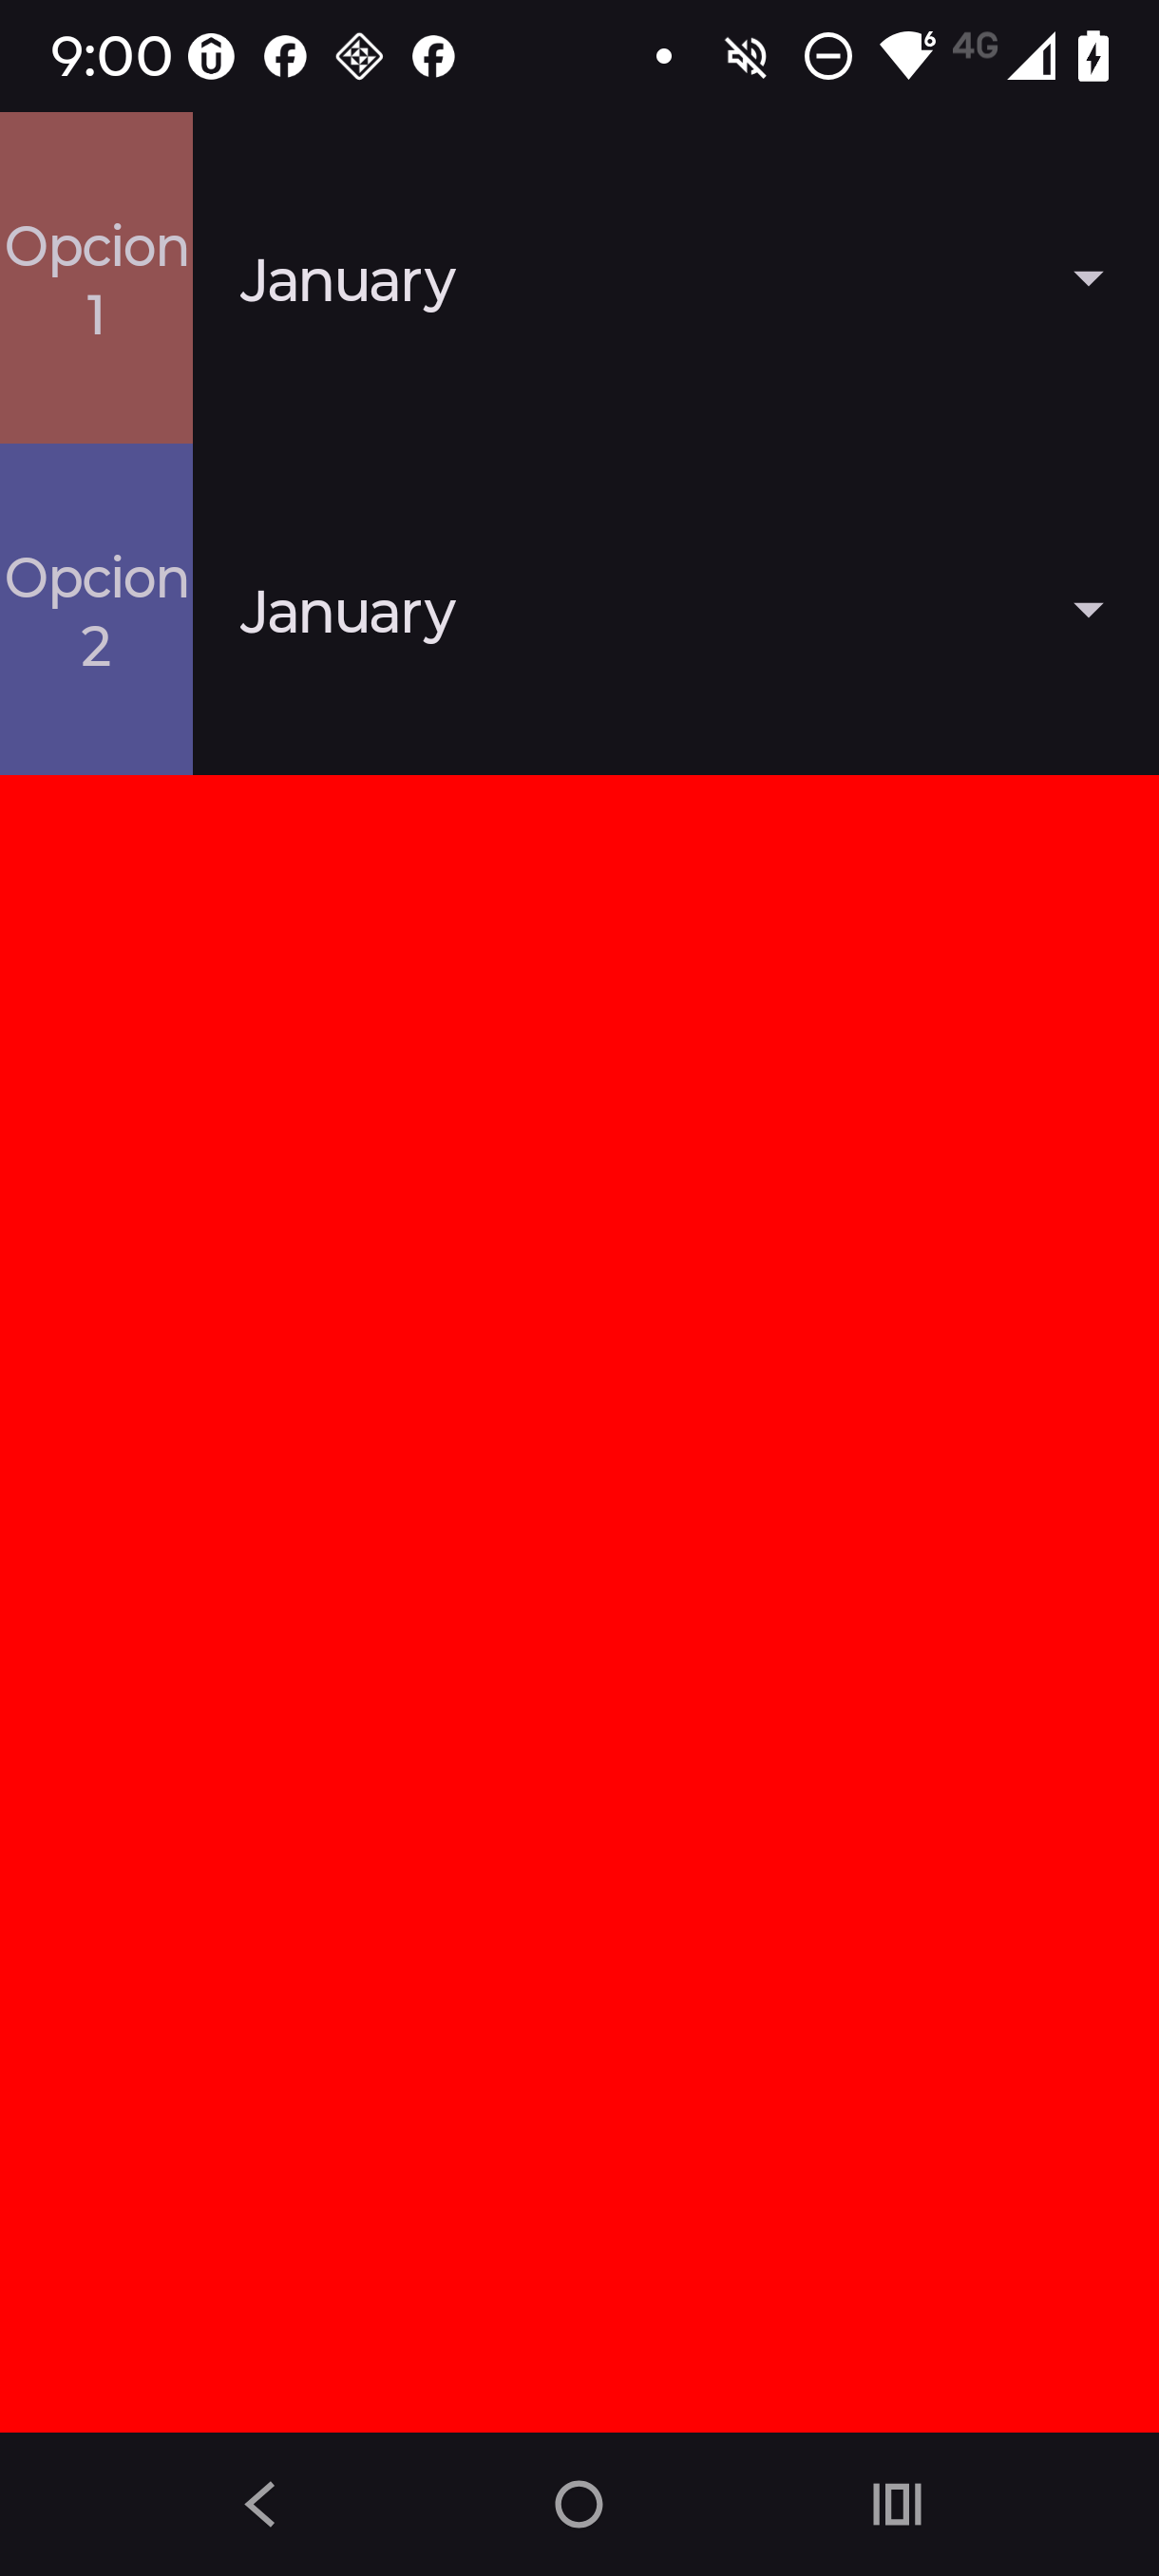
\includegraphics[width=0.98\textwidth]{02_TallerCBTis/figs/Demo07}
\end{center}

\end{columns}

\end{frame}




\begin{frame}{Componente SeekBar en Android}
\textbf{¿Qué es un SeekBar?}

\begin{itemize}
    \item Es un componente de interfaz gráfica que permite al usuario seleccionar un valor dentro de un rango deslizando un control horizontal.
    \item Es una extensión de la clase ProgressBar con interacción del usuario.
\end{itemize}

\vspace{0.5cm}

\textbf{¿Para qué sirve?}
\begin{itemize}
    \item Ajustar valores continuos o discretos (ej. volumen, brillo, progreso).
    \item Permitir entrada intuitiva mediante deslizamiento.
    \item Controlar parámetros en tiempo real.
\end{itemize}

\vspace{0.5cm}

\textbf{Características principales:}
\begin{itemize}
    \item Permite definir valores mínimo, máximo y progreso actual.
    \item Puede escuchar cambios mediante un listener (OnSeekBarChangeListener).
    \item Es altamente personalizable (colores, tamaño, estilo).
\end{itemize}


\end{frame}


\begin{frame}[fragile]
\frametitle{Demo 08: Agregar SeekBars}
\begin{columns}
\column{0.80\linewidth}
Del Repositorio Github:
\begin{itemize}
\item Copiar el archivo MainActivity\_Demo08.java (dentro del Folder códigosJAVA) al mismo directorio donde esta el MainActivity.java
\item Copiar el archivo activity\_main\_demo08.xml (dentro del Folder Carpeta\_layout) al mismo directorio donde esta el activity\_main.xml
%\item Copiar los archivos \textit{cgup.jpg} y \textit{logo\_upv\_2019.png} localizados dentro de la folder \textit{Carpeta\_drawable} en el directorio \textit{res/drawable} del proyecto de AS.
\item Modificar en el archivo AndroidManifest.xml la cadena \textit{.MainActivity\_Demo07} por \textit{.MainActivity\_Demo08}
\end{itemize}

\begin{block}{Demo \#08}
Muestra una App dos SeekBars (la segunda utiliza separadores finitos). La primera SeekBar actualiza el contenido de TextView conforme la seleccion del usuario. 
\end{block}


\column{0.20\linewidth}

\begin{center}
 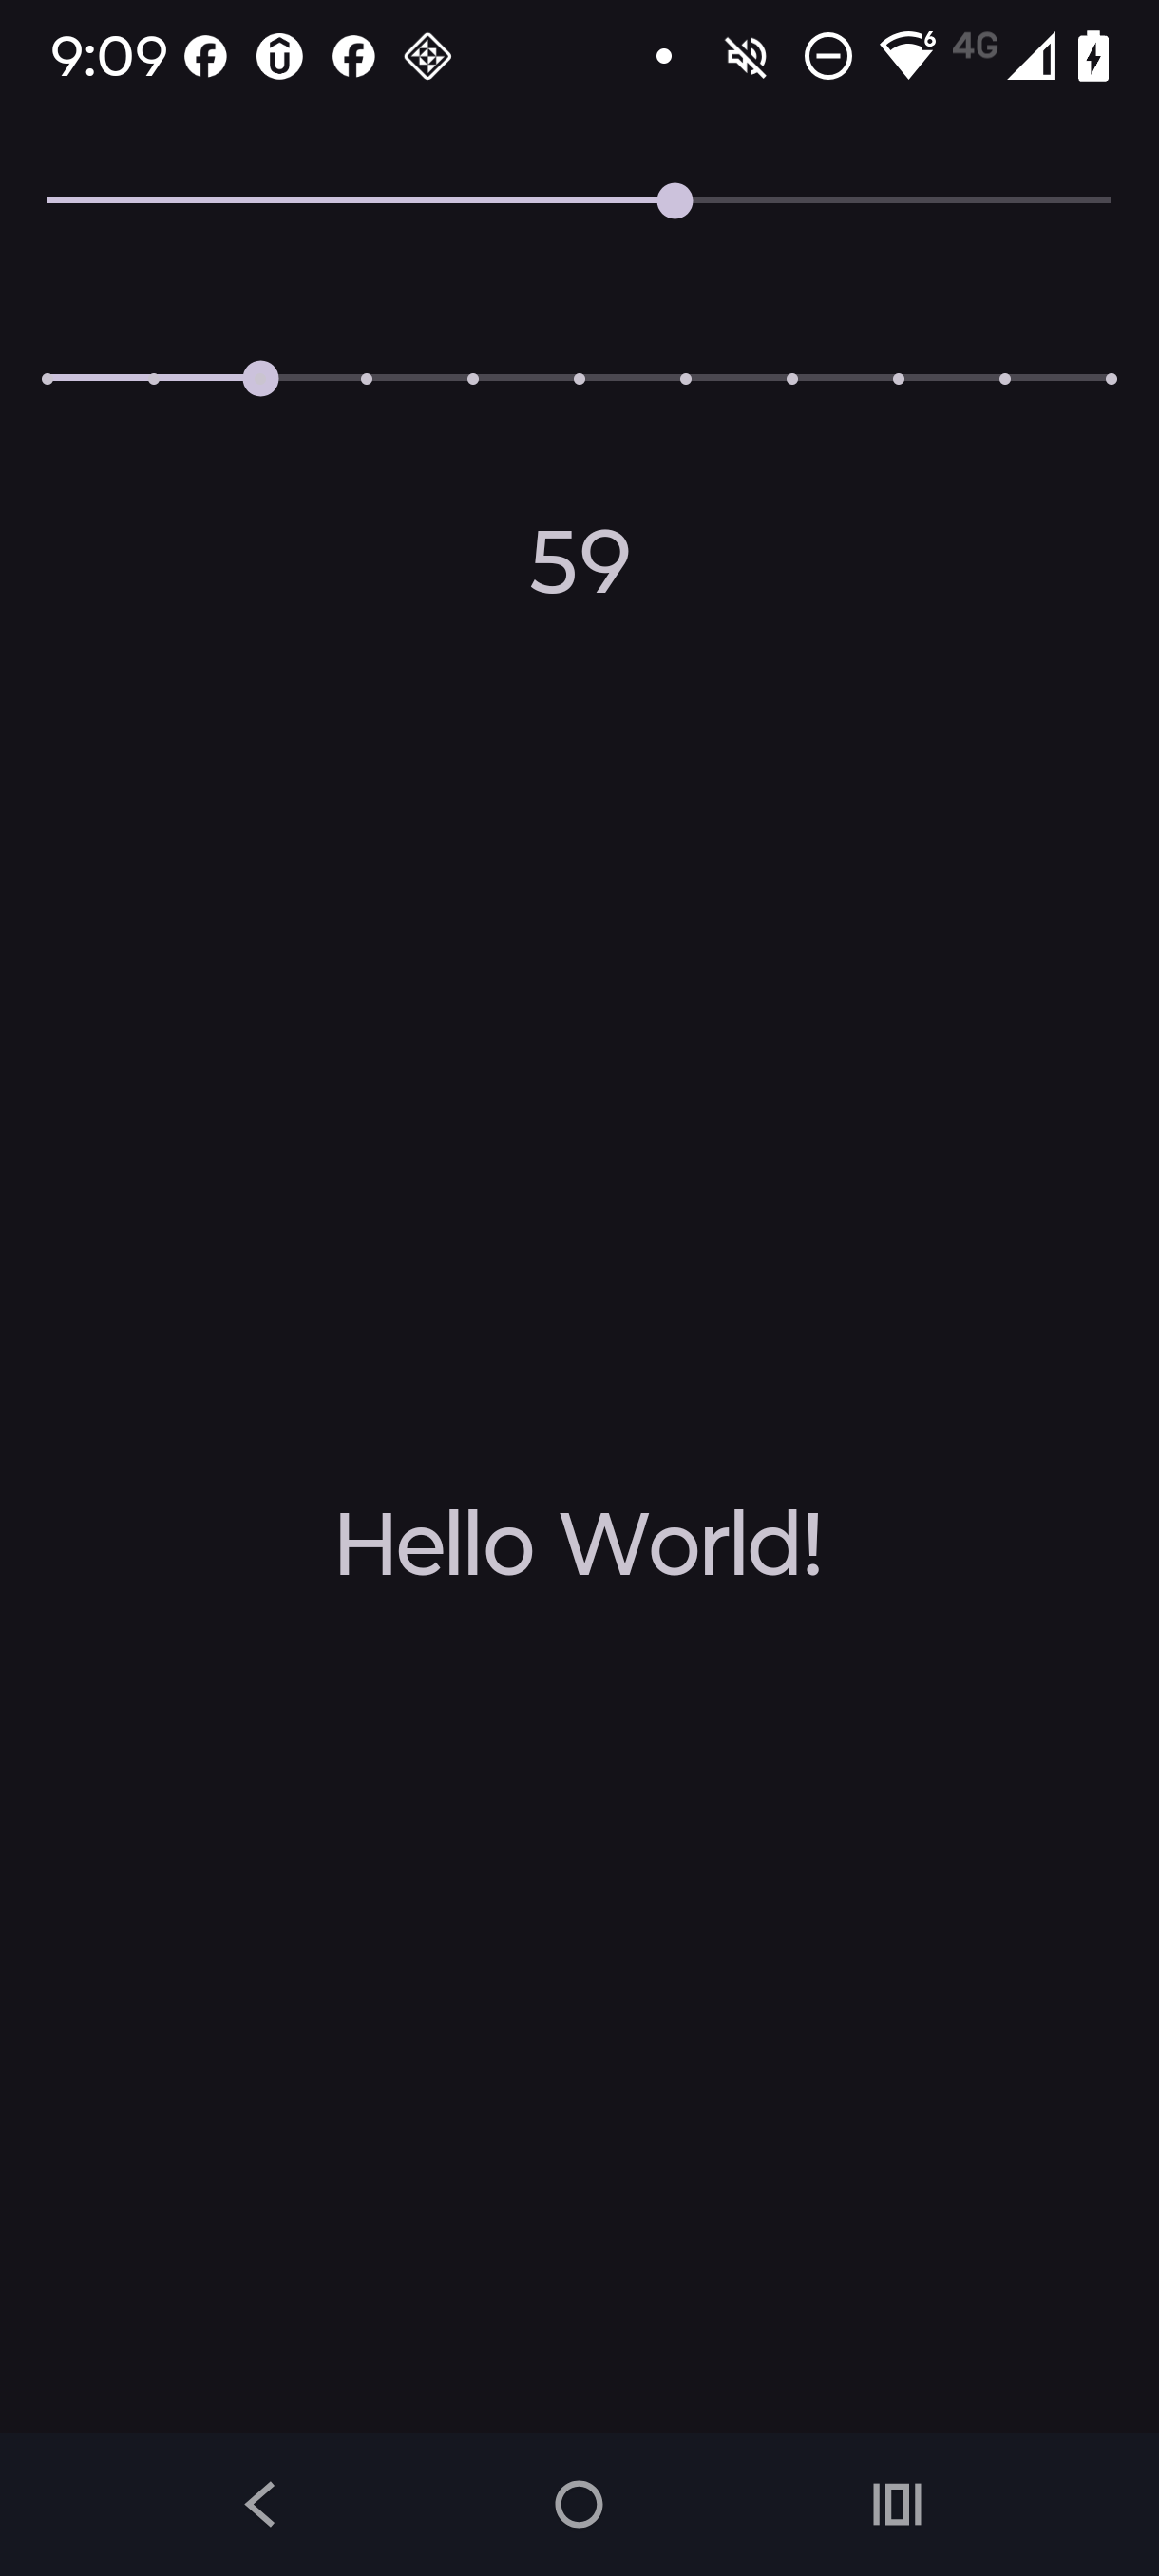
\includegraphics[width=0.98\textwidth]{02_TallerCBTis/figs/Demo08}
\end{center}

\end{columns}

\end{frame}




%\end{document}

%
\begin{frame}{Componente SeekBar en Android}
\textbf{¿Qué es un SeekBar?}

\begin{itemize}
    \item Es un componente de interfaz gráfica que permite al usuario seleccionar un valor dentro de un rango deslizando un control horizontal.
    \item Es una extensión de la clase ProgressBar con interacción del usuario.
\end{itemize}

\vspace{0.5cm}

\textbf{¿Para qué sirve?}
\begin{itemize}
    \item Ajustar valores continuos o discretos (ej. volumen, brillo, progreso).
    \item Permitir entrada intuitiva mediante deslizamiento.
    \item Controlar parámetros en tiempo real.
\end{itemize}

\vspace{0.5cm}

\textbf{Características principales:}
\begin{itemize}
    \item Permite definir valores mínimo, máximo y progreso actual.
    \item Puede escuchar cambios mediante un listener (OnSeekBarChangeListener).
    \item Es altamente personalizable (colores, tamaño, estilo).
\end{itemize}


\end{frame}


\begin{frame}[fragile]
\frametitle{Demo 08: Agregar SeekBars}
\begin{columns}
\column{0.80\linewidth}
Del Repositorio Github:
\begin{itemize}
\item Copiar el archivo MainActivity\_Demo08.java (dentro del Folder códigosJAVA) al mismo directorio donde esta el MainActivity.java
\item Copiar el archivo activity\_main\_demo08.xml (dentro del Folder Carpeta\_layout) al mismo directorio donde esta el activity\_main.xml
%\item Copiar los archivos \textit{cgup.jpg} y \textit{logo\_upv\_2019.png} localizados dentro de la folder \textit{Carpeta\_drawable} en el directorio \textit{res/drawable} del proyecto de AS.
\item Modificar en el archivo AndroidManifest.xml la cadena \textit{.MainActivity\_Demo07} por \textit{.MainActivity\_Demo08}
\end{itemize}

\begin{block}{Demo \#08}
Muestra una App dos SeekBars (la segunda utiliza separadores finitos). La primera SeekBar actualiza el contenido de TextView conforme la seleccion del usuario. 
\end{block}


\column{0.20\linewidth}

\begin{center}
 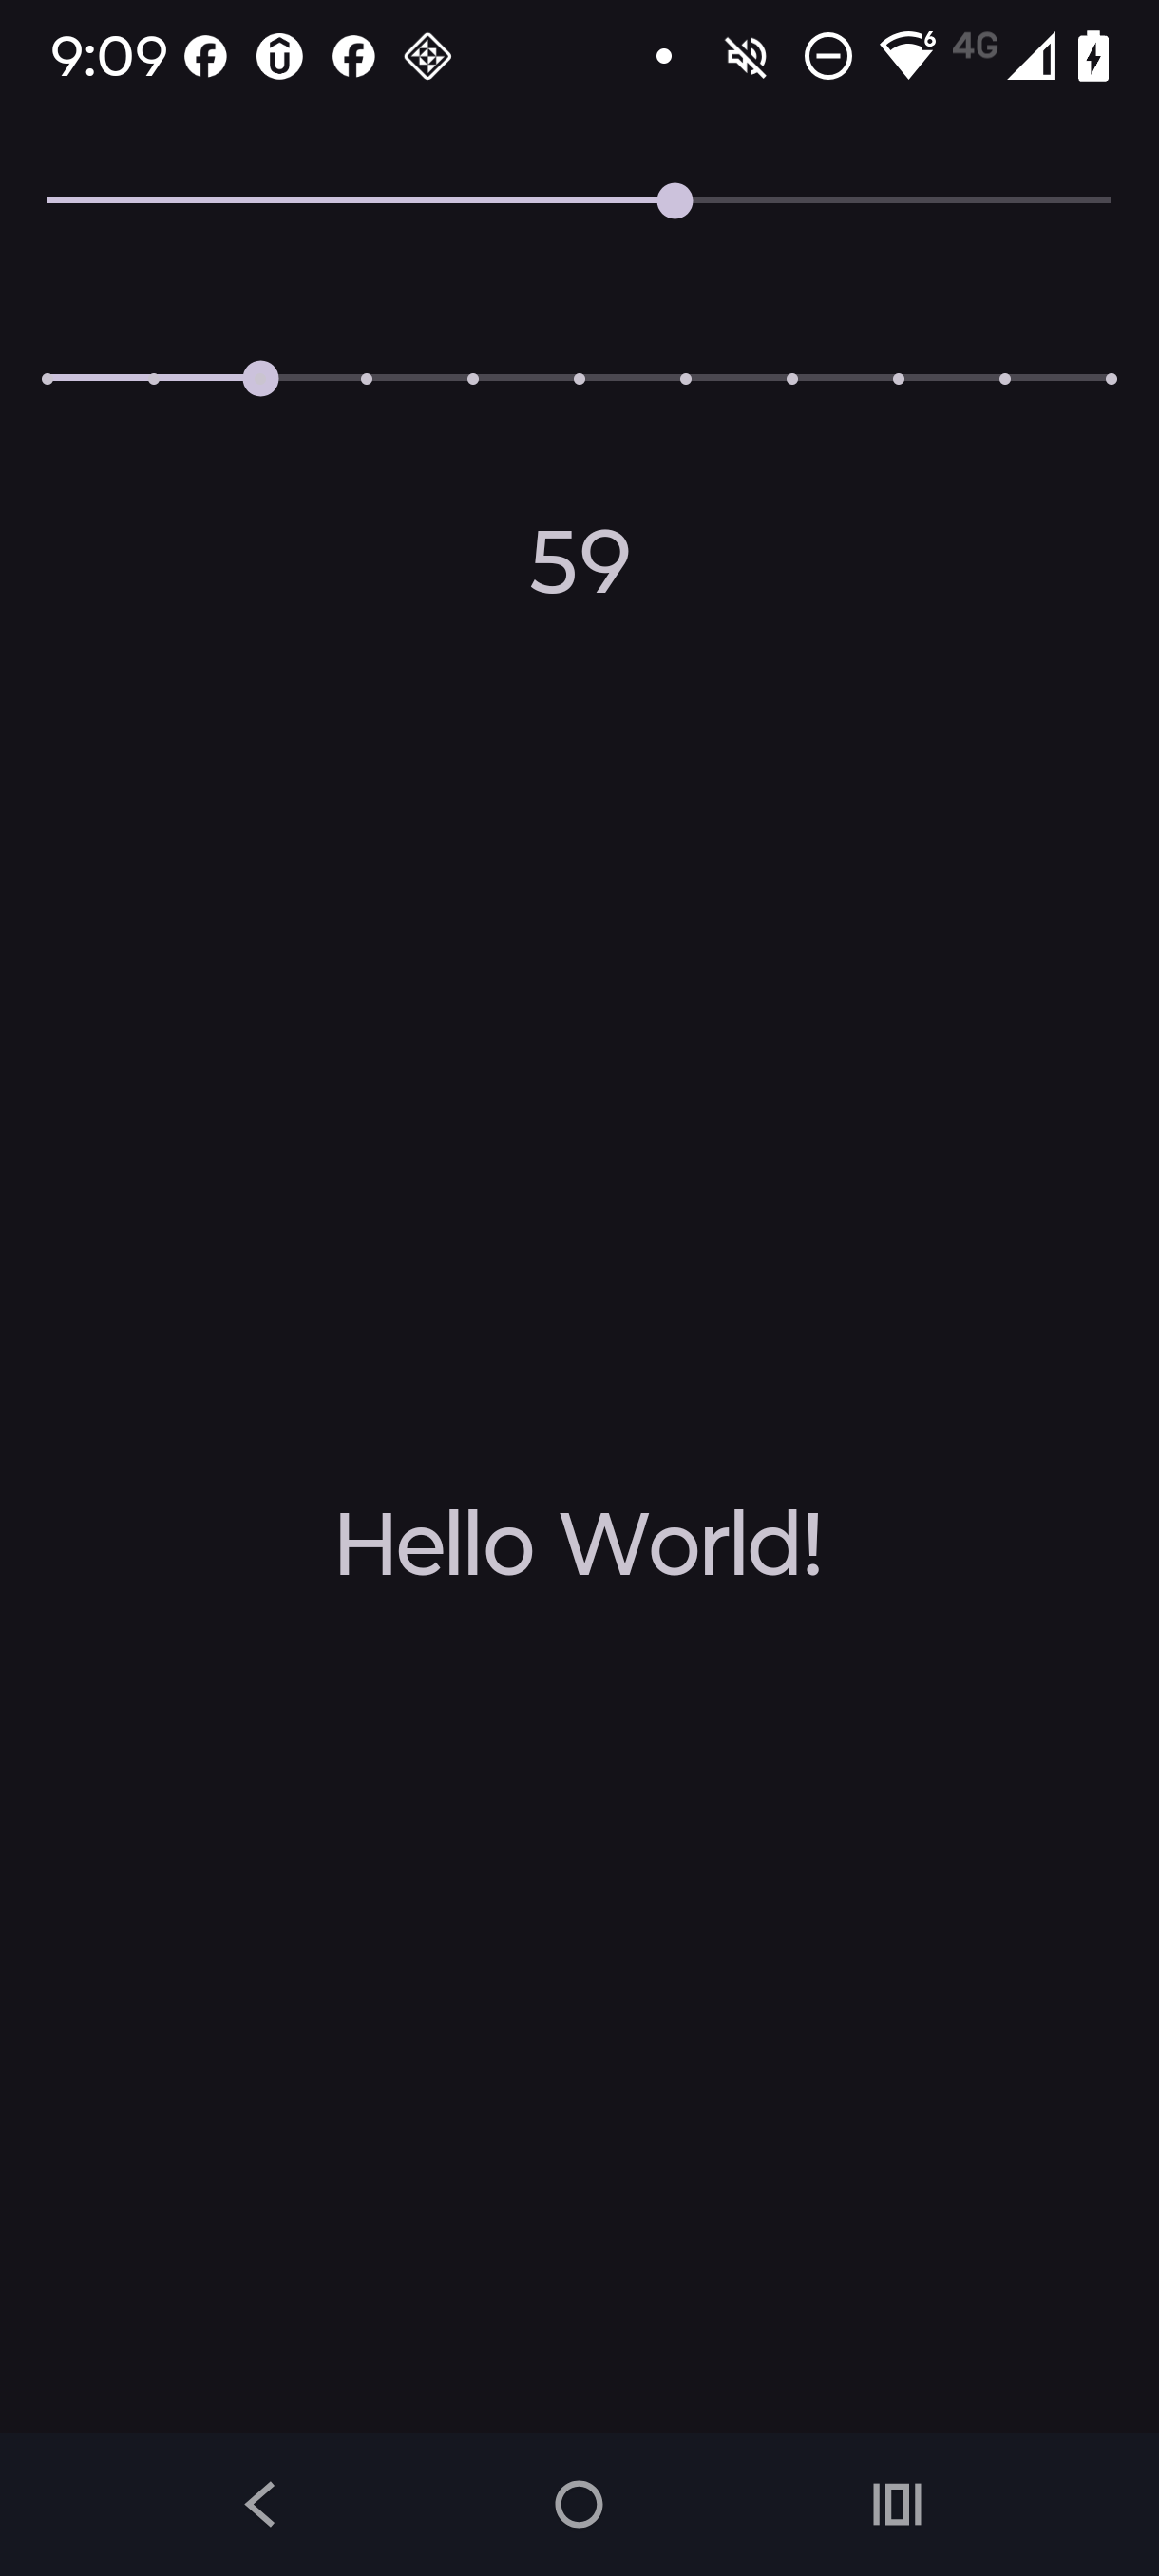
\includegraphics[width=0.98\textwidth]{02_TallerCBTis/figs/Demo08}
\end{center}

\end{columns}

\end{frame}



%\begin{frame}{startActivityForResult y onActivityResult}


\begin{frame}[fragile]
\frametitle{startActivityForResult y onActivityResult}  
\textbf{¿Para qué sirven?}

\begin{itemize}
    \item Permiten iniciar una actividad esperando un resultado de regreso.
    \item Son útiles cuando se necesita que una segunda pantalla devuelva información (por ejemplo, selección de datos o confirmaciones).
\end{itemize}

\vspace{0.4cm}

\textbf{Flujo de funcionamiento:}
\begin{enumerate}
    \item Se inicia la actividad con \texttt{startActivityForResult()}.
    \item La segunda actividad procesa la información.
    \item Se devuelve un resultado mediante \texttt{setResult()}.
    \item La actividad original recibe el resultado en \texttt{onActivityResult()}.
\end{enumerate}


\textbf{Ejemplo en Java:}
\begin{block}{}
\small
\begin{minted}[linenos,fontsize=\tiny]{java}
// Lanzar actividad
Intent intent = new Intent(this, SegundaActivity.class);
startActivityForResult(intent, 1);

// Recibir resultado
@Override
protected void onActivityResult(int requestCode, int resultCode, Intent data) {
    if (requestCode == 1 && resultCode == RESULT_OK) {
        String resultado = data.getStringExtra("dato");
    }
}
\end{minted}
\end{block}

\end{frame}




\begin{frame}[fragile]
\frametitle{Demo 09: Lectura y Escritura de Archivos de Texto}
\begin{columns}
\column{0.80\linewidth}
Del Repositorio Github:
\begin{itemize}
\item Copiar el archivo \textit{MainActivity\_Demo09.java} (dentro del Folder códigosJAVA) al mismo directorio donde esta el MainActivity.java
\item Copiar el archivo \textit{activity\_main\_demo09.xml} (dentro del Folder Carpeta\_layout) al mismo directorio donde esta el activity\_main.xml

%\item Copiar los archivos \textit{cgup.jpg} y \textit{logo\_upv\_2019.png} localizados dentro de la folder \textit{Carpeta\_drawable} en el directorio \textit{res/drawable} del proyecto de AS.
\item Modificar en el archivo \textit{AndroidManifest.xml} la cadena \textit{.MainActivity\_Demo08} por \textit{.MainActivity\_Demo09}.
\item Ir a la linea 22 de archivo del archivo \textit{MainActivity\_Demo09.java}, poner el cursos en la palabra (en Rojo) \textit{documentfile}, presionar la combinación ALT+ENTER, y seleccionar de la lista desplegable la opcion ``Add dependency on ....''. Esto quitará el error y hara los ajustes necesarios. 
\end{itemize}

%\begin{block}{Demo \#09}
%Un App que permite escribir el contenido de un EditText a un archivo y cargar el contenido de cualquier archivo en el EditText
%\end{block}


\column{0.20\linewidth}

\begin{center}
 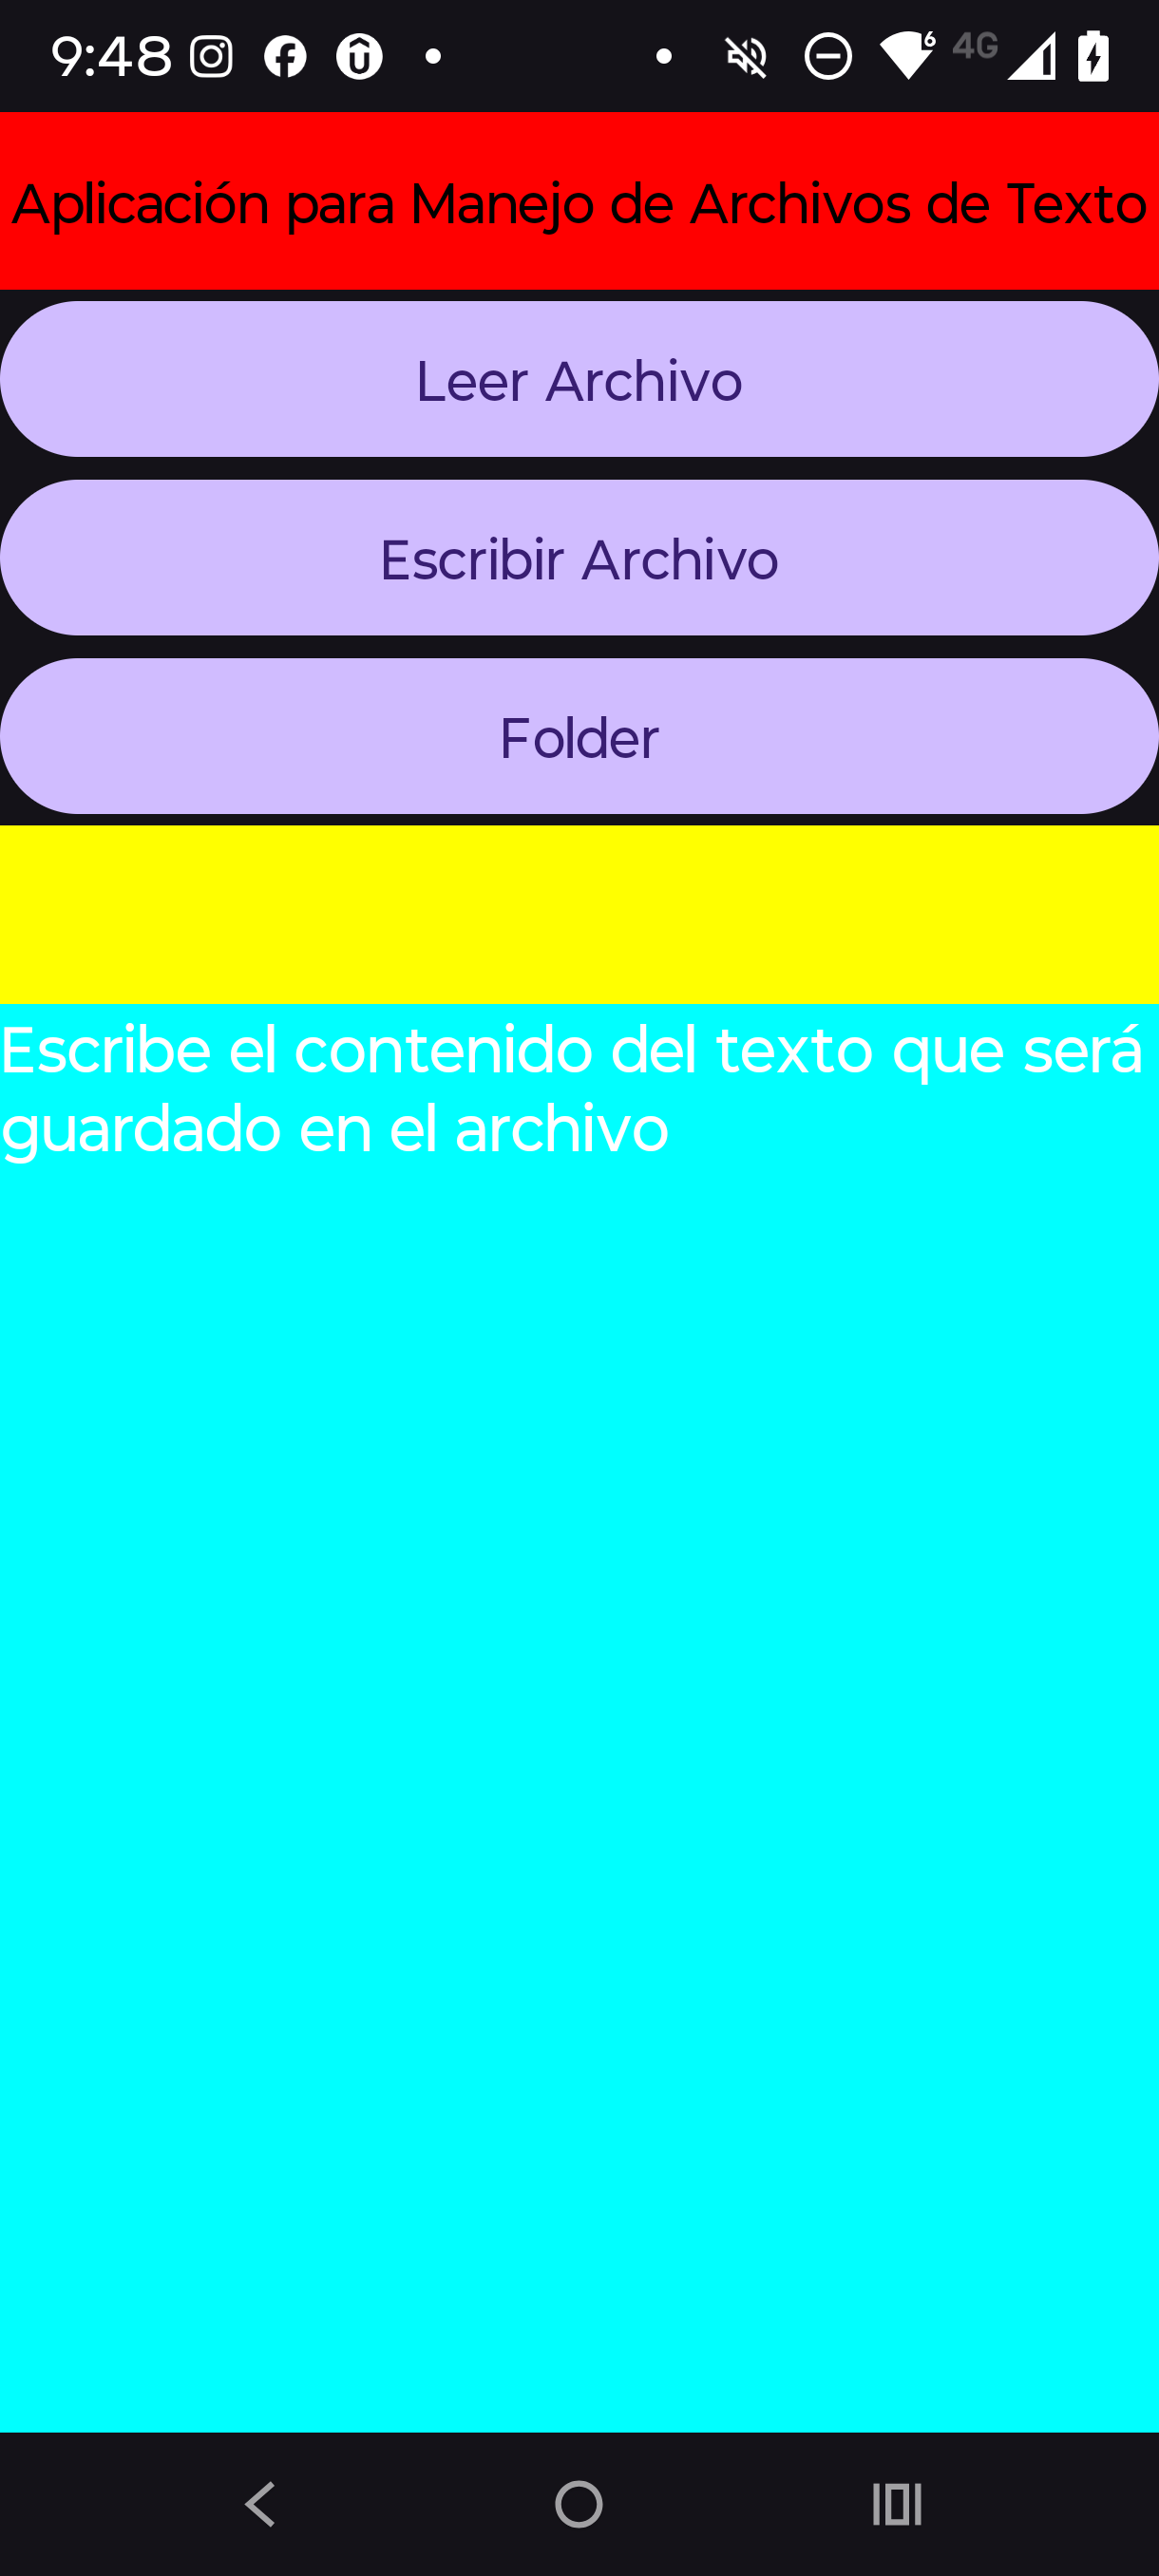
\includegraphics[width=0.98\textwidth]{02_TallerCBTis/figs/Demo09}
\end{center}

\end{columns}

\end{frame}




\begin{frame}[fragile]
\frametitle{startActivityForResult y onActivityResult}

\textbf{¿Para qué sirven?}

\begin{itemize}
    \item Permiten iniciar una actividad esperando un resultado de regreso.
    \item Son útiles cuando se necesita que una segunda pantalla devuelva información (por ejemplo, selección de datos o confirmaciones).
\end{itemize}

\textbf{Flujo de funcionamiento:}
\begin{enumerate}
    \item Se inicia la actividad con \texttt{startActivityForResult()}.
    \item La segunda actividad procesa la información.
    \item Se devuelve un resultado mediante \texttt{setResult()}.
    \item La actividad original recibe el resultado en \texttt{onActivityResult()}.
\end{enumerate}

\textbf{Ejemplo en Java:}

%\begin{block}{Archivo \textbf{activity\_main.xml}}
\begin{minted}[linenos,fontsize=\tiny]{java}
// Lanzar actividad
Intent intent = new Intent(this, SegundaActivity.class);
startActivityForResult(intent, 1);

// Recibir resultado
@Override
protected void onActivityResult(int requestCode, int resultCode, Intent data) {
    if (requestCode == 1 && resultCode == RESULT_OK) {
        String resultado = data.getStringExtra("dato");
    }
}
\end{minted}

%\end{block}
\end{frame}


\begin{frame}{Lectura de Archivos en Android (Java)}
\textbf{Método: readFromFile(Uri uri, String text)}

\begin{itemize}
    \item Este método permite leer el contenido de un archivo a partir de una \textbf{URI}.
    \item Utiliza el \textbf{ContentResolver} para acceder a recursos externos.
\end{itemize}


\textbf{Flujo del código:}
\begin{enumerate}
    \item Se obtiene un flujo de entrada:
    \begin{itemize}
        \item \texttt{InputStream is = getContentResolver().openInputStream(uri);}
    \end{itemize}
    
    \item Se crea un lector de texto:
    \begin{itemize}
        \item \texttt{BufferedReader bf = new BufferedReader(new InputStreamReader(is));}
    \end{itemize}
    
    \item Se lee el archivo línea por línea:
    \begin{itemize}
        \item Se usa un ciclo \texttt{while} para concatenar el contenido en una variable.
    \end{itemize}
    
    \item Se muestra el contenido en pantalla:
    \begin{itemize}
        \item Se obtiene un \texttt{TextView} con \texttt{findViewById}.
        \item Se asigna el texto con \texttt{setText(FileContents)}.
    \end{itemize}
\end{enumerate}


\textbf{Manejo de errores:}
\begin{itemize}
    \item Se utiliza un bloque \texttt{try-catch} para capturar excepciones \texttt{IOException}.
\end{itemize}

\end{frame}


\begin{frame}{Escritura de Archivos en Android}
\textbf{Método: writeInFile(...)}

\begin{itemize}
    \item Este método permite escribir texto en un archivo identificado por una URI.
    \item Utiliza flujos de salida (\textit{OutputStream}) para manejar la escritura.
\end{itemize}


\textbf{Parámetros:}
\begin{itemize}
    \item \textbf{Uri uri:} Dirección del archivo donde se escribirá el contenido.
    \item \textbf{String text:} Texto que se desea guardar.
\end{itemize}


\textbf{Funcionamiento:}
\begin{itemize}
    \item Se obtiene un \textbf{OutputStream} mediante \texttt{getContentResolver()}.
    \item Se envuelve en un \textbf{BufferedWriter} para escribir texto eficientemente.
    \item Se escribe el contenido con \texttt{write(text)}.
    \item Se asegura la escritura con \texttt{flush()}.
    \item Se cierra el flujo con \texttt{close()}.
\end{itemize}


\textbf{Manejo de errores:}
\begin{itemize}
    \item Se utiliza un bloque \texttt{try-catch} para capturar excepciones de tipo \texttt{IOException}.
\end{itemize}


\end{frame}


\begin{frame}[fragile]
\frametitle{Demo 09: Lectura y Escritura de Archivos de Texto}
\begin{columns}
\column{0.80\linewidth}
Del Repositorio Github:
\begin{itemize}
\item Copiar el archivo \textit{MainActivity\_Demo09.java} (dentro del Folder códigosJAVA) al mismo directorio donde esta el MainActivity.java
\item Copiar el archivo \textit{activity\_main\_demo09.xml} (dentro del Folder Carpeta\_layout) al mismo directorio donde esta el activity\_main.xml

%\item Copiar los archivos \textit{cgup.jpg} y \textit{logo\_upv\_2019.png} localizados dentro de la folder \textit{Carpeta\_drawable} en el directorio \textit{res/drawable} del proyecto de AS.
\item Modificar en el archivo \textit{AndroidManifest.xml} la cadena \textit{.MainActivity\_Demo08} por \textit{.MainActivity\_Demo09}.
\item Ir a la linea 22 de archivo del archivo \textit{MainActivity\_Demo09.java}, poner el cursos en la palabra (en Rojo) \textit{documentfile}, presionar la combinación ALT+ENTER, y seleccionar de la lista desplegable la opcion ``Add dependency on ....''. Esto quitará el error y hara los ajustes necesarios. 
\end{itemize}

%\begin{block}{Demo \#09}
%Un App que permite escribir el contenido de un EditText a un archivo y cargar el contenido de cualquier archivo en el EditText
%\end{block}


\column{0.20\linewidth}

\begin{center}
 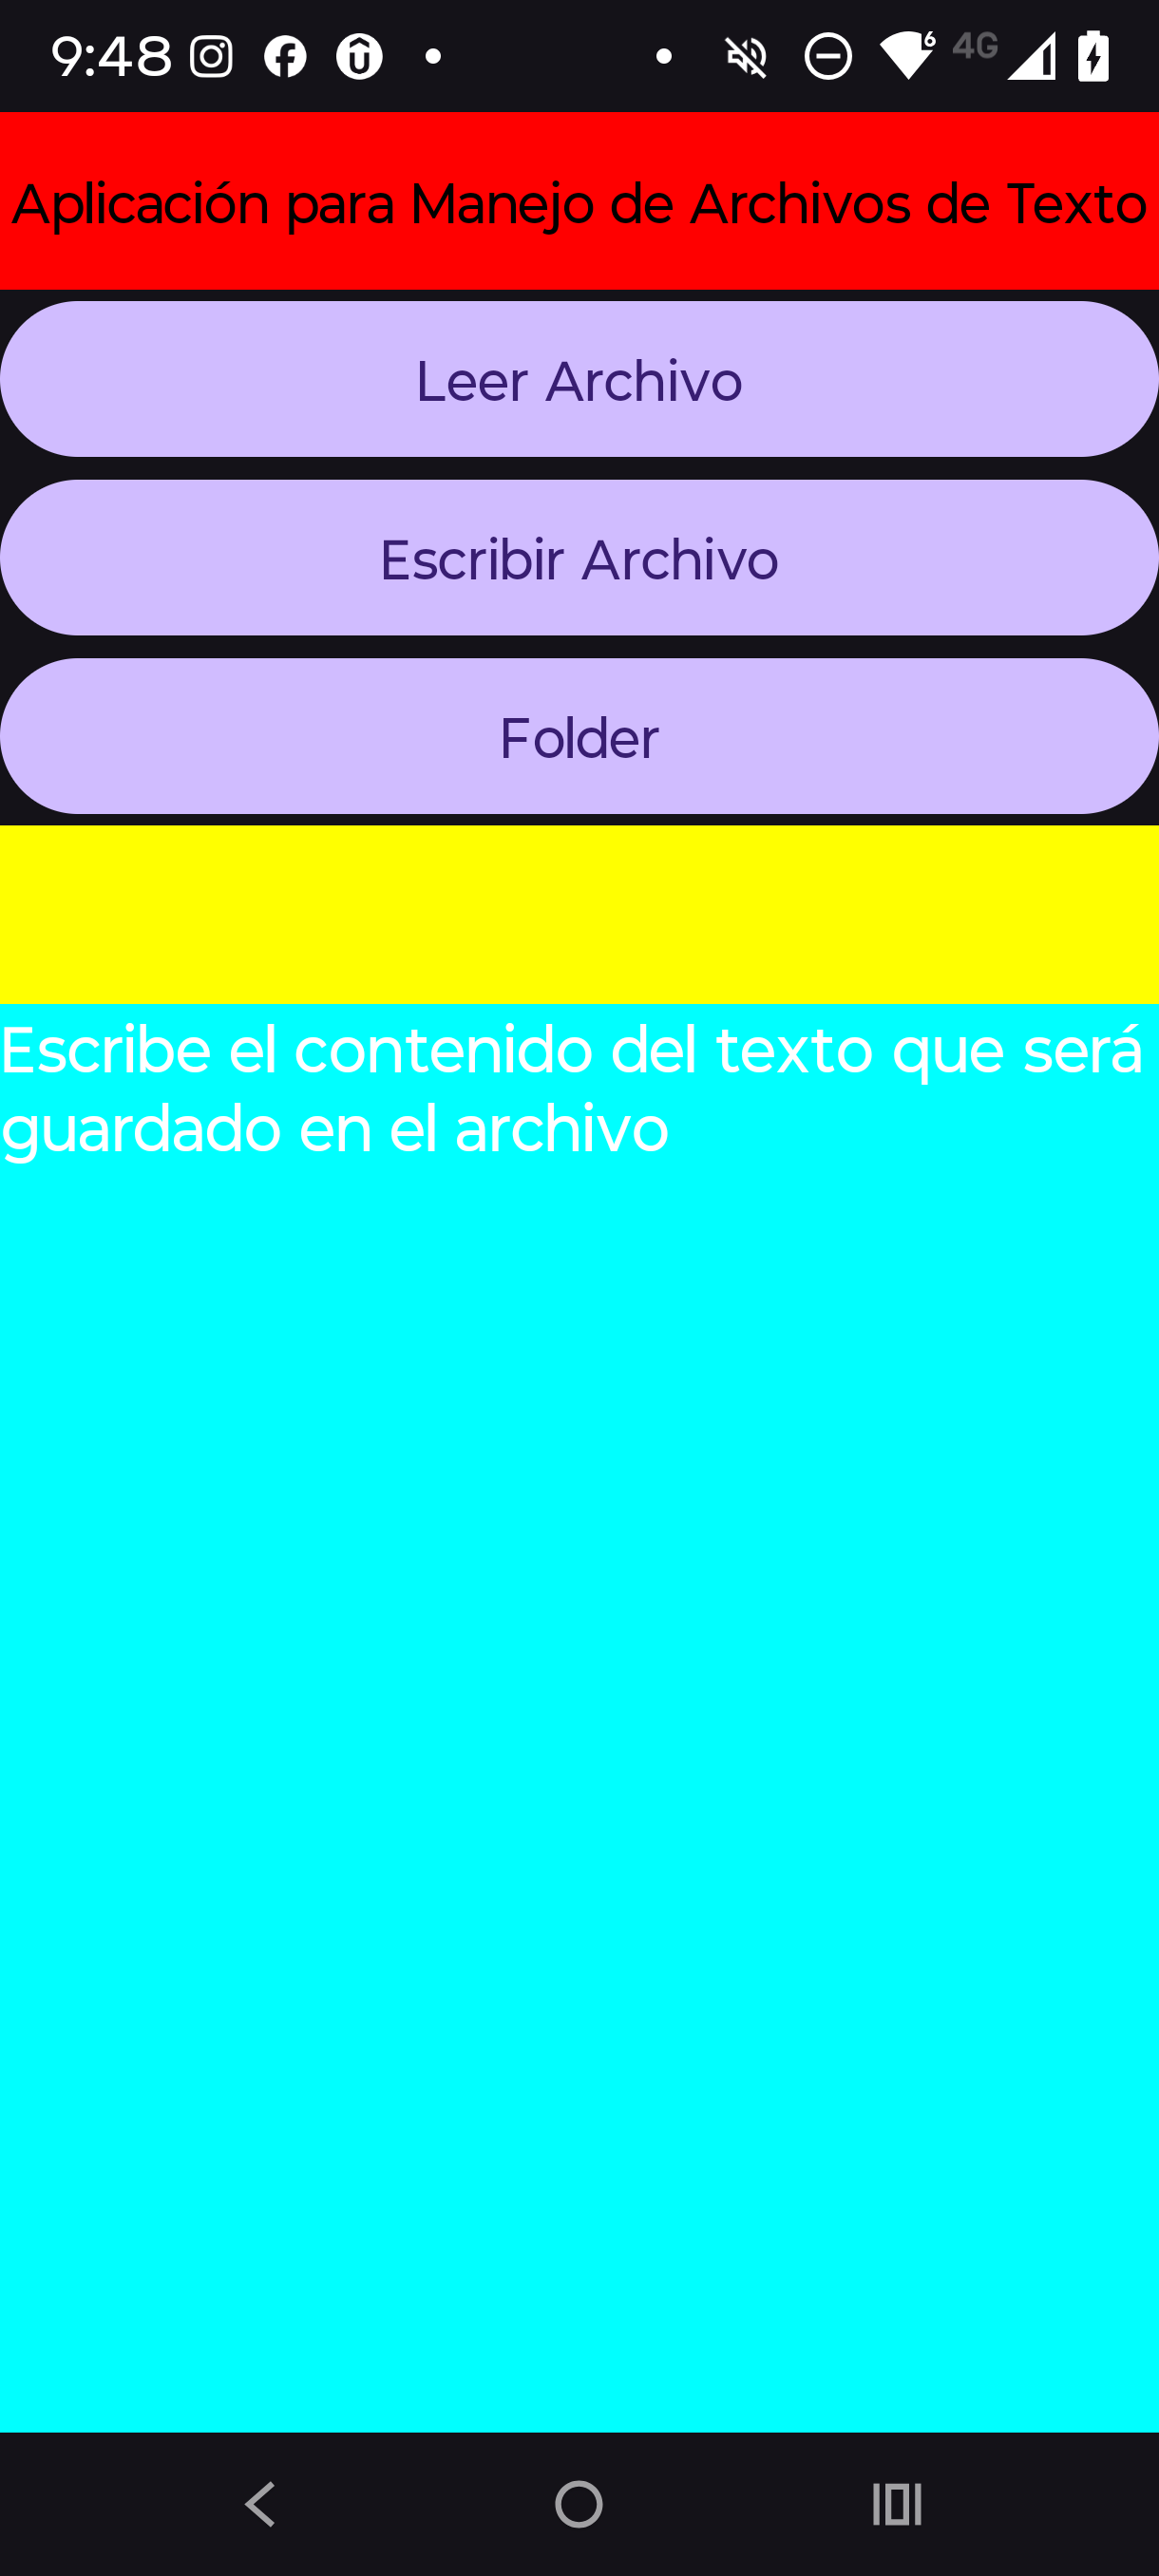
\includegraphics[width=0.98\textwidth]{02_TallerCBTis/figs/Demo09}
\end{center}

\end{columns}

\end{frame}


\begin{frame}[fragile]{ProgressDialog en Android}
\textbf{¿Qué es ProgressDialog?}

\begin{itemize}
    \item Es un componente utilizado para mostrar un indicador de progreso al usuario.
    \item Se emplea comúnmente durante operaciones largas (carga de datos, procesos en segundo plano).
\end{itemize}


\textbf{Características:}
\begin{itemize}
    \item Puede mostrar un mensaje informativo.
    \item Puede ser cancelable o no por el usuario.
    \item Soporta estilos como barra de progreso o spinner.
\end{itemize}

\end{frame}


\begin{frame}[fragile]{Uso de AsyncTask para tareas en segundo plano}
\textbf{Clase: DownloadTask extends AsyncTask$<$String, Integer, List$<$String$>$$>$}

\begin{itemize}
    \item Permite ejecutar tareas en segundo plano sin bloquear la interfaz gráfica.
    \item Usa tres tipos genéricos:
    \begin{itemize}
        \item \textbf{String:} parámetros de entrada.
        \item \textbf{Integer:} progreso.
        \item \textbf{List$<$String$>$:} resultado final.
    \end{itemize}
\end{itemize}

\vspace{0.3cm}

\textbf{Fases del AsyncTask:}
\begin{itemize}
    \item \textbf{onPreExecute():} Inicializa variables y muestra el ProgressDialog.
    \item \textbf{doInBackground():} Ejecuta tareas en segundo plano, publica progreso y simula espera.
    \item \textbf{onProgressUpdate():} Actualiza la barra de progreso y mensaje.
    \item \textbf{onPostExecute():} Oculta el diálogo y muestra resultados en pantalla.
\end{itemize}



\end{frame}


\begin{frame}[fragile]
\frametitle{Demo 10: Progress Dialog y AsyncTask}
\begin{columns}
\column{0.80\linewidth}
Del Repositorio Github:
\begin{itemize}
\item Copiar el archivo \textit{MainActivity\_Demo10.java} (dentro del Folder códigosJAVA) al mismo directorio donde esta el MainActivity.java
\item Copiar el archivo \textit{activity\_main\_demo10.xml} (dentro del Folder Carpeta\_layout) al mismo directorio donde esta el activity\_main.xml
%\item Copiar los archivos \textit{cgup.jpg} y \textit{logo\_upv\_2019.png} localizados dentro de la folder \textit{Carpeta\_drawable} en el directorio \textit{res/drawable} del proyecto de AS.
\item Modificar en el archivo \textit{AndroidManifest.xml} la cadena \textit{.MainActivity\_Demo09} por \textit{.MainActivity\_Demo10}.
%\item Ir a la linea 22 de archivo del archivo \textit{MainActivity\_Demo09.java}, poner el cursos en la palabra (en Rojo) \textit{documentfile}, presionar la combinación ALT+ENTER, y seleccionar de la lista desplegable la opcion ``Add dependency on ....''. Esto quitará el error y hara los ajustes necesarios. 
\end{itemize}

%\begin{block}{Demo \#09}
%Un App que permite escribir el contenido de un EditText a un archivo y cargar el contenido de cualquier archivo en el EditText
%\end{block}


\column{0.20\linewidth}

\begin{center}
 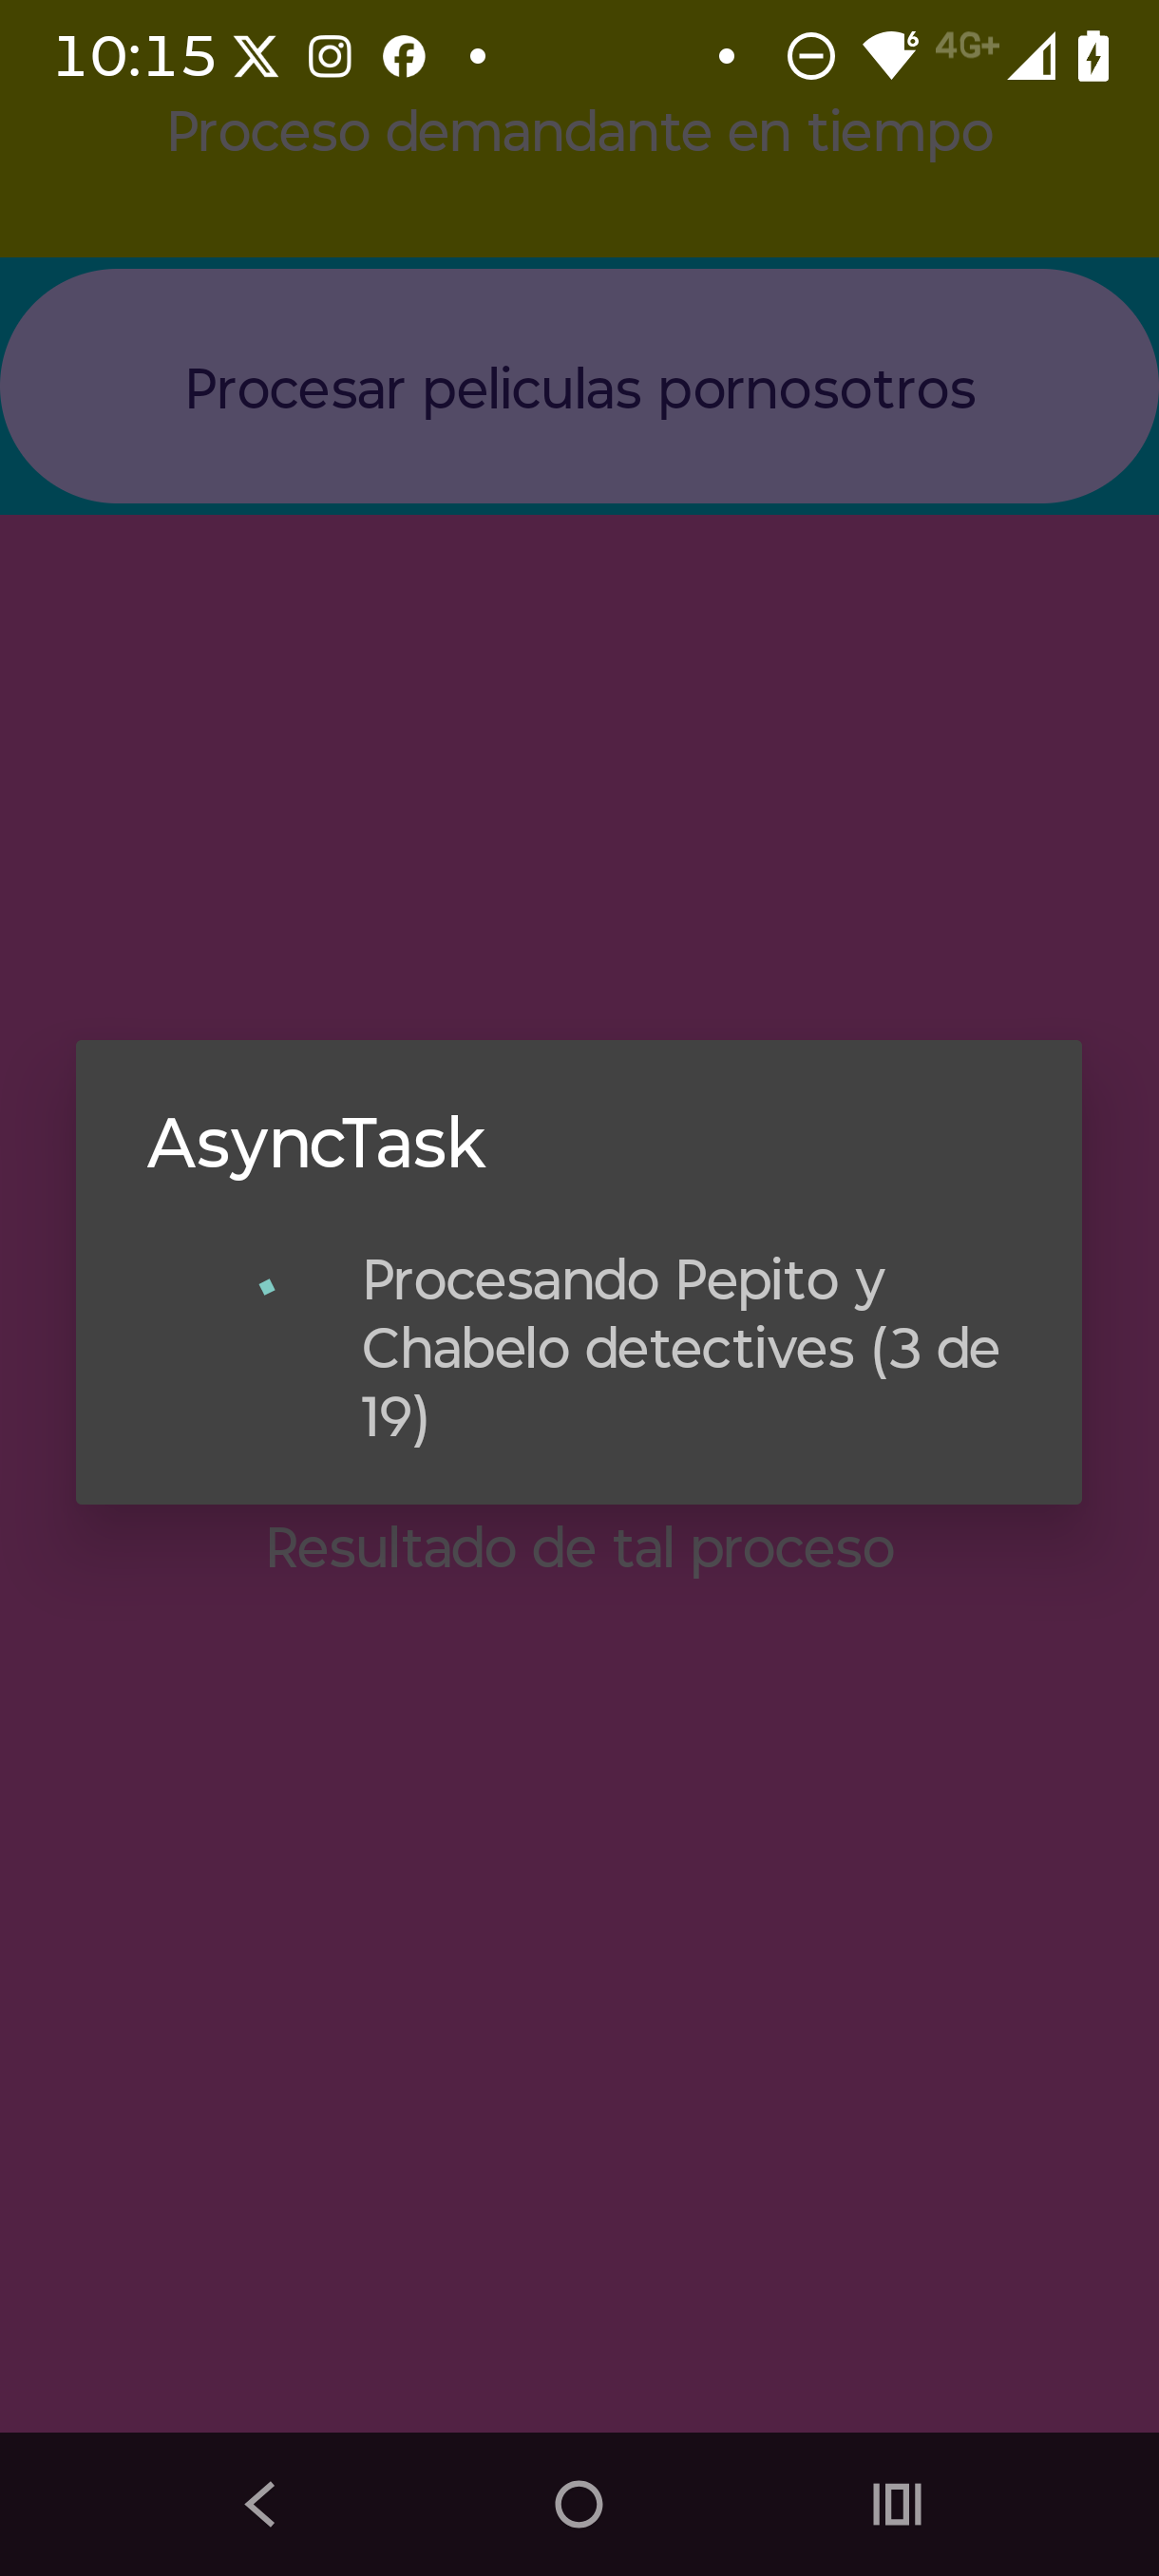
\includegraphics[width=0.98\textwidth]{02_TallerCBTis/figs/Demo10}
\end{center}

\end{columns}

\end{frame}


\begin{frame}[fragile]{AlertDialog.Builder y Dialog con XML en Android}

\textbf{¿Qué es un Cuadro de Dialogo?} 
\begin{itemize} 
\item Es una ventana emergente que permite interactuar con el usuario. 
\end{itemize}

\textbf{¿Qué es AlertDialog.Builder?}
\begin{itemize}
    \item Clase utilizada para construir y mostrar diálogos emergentes.
    \item Permite definir título, mensaje, botones y eventos.
\end{itemize}


\textbf{Dialog con contenido XML:}
\begin{itemize}
    \item Permite usar una interfaz personalizada definida en un layout XML.
    \item Se establece su contenido en base al archivo XML.
\end{itemize}


\textbf{Ventajas del Dialogo Personalizado:}
\begin{itemize}
    \item Mayor personalización de la interfaz.
    \item Permite incluir EditText, imágenes, botones, etc.
\end{itemize}

\end{frame}



\begin{frame}[fragile]
\frametitle{Demo 11: Dialog y CustoDialog}
\begin{columns}
\column{0.80\linewidth}
Del Repositorio Github:
\begin{itemize}
\item Copiar el archivo \textit{MainActivity\_Demo11.java} (dentro del Folder códigosJAVA) al mismo directorio donde esta el MainActivity.java
\item Copiar el archivo \textit{activity\_main\_demo11.xml} (dentro del Folder Carpeta\_layout) al mismo directorio donde esta el activity\_main.xml
\item Copiar el archivo \textit{custom\_dialog.xml} (dentro del Folder Carpeta\_layout) al mismo directorio donde esta el activity\_main.xml.
\item Modificar en el archivo \textit{AndroidManifest.xml} la cadena \textit{.MainActivity\_Demo10} por \textit{.MainActivity\_Demo11}.
%\item Ir a la linea 22 de archivo del archivo \textit{MainActivity\_Demo09.java}, poner el cursos en la palabra (en Rojo) \textit{documentfile}, presionar la combinación ALT+ENTER, y seleccionar de la lista desplegable la opcion ``Add dependency on ....''. Esto quitará el error y hara los ajustes necesarios. 
\end{itemize}

%\begin{block}{Demo \#09}
%Un App que permite escribir el contenido de un EditText a un archivo y cargar el contenido de cualquier archivo en el EditText
%\end{block}


\column{0.20\linewidth}

\begin{center}
 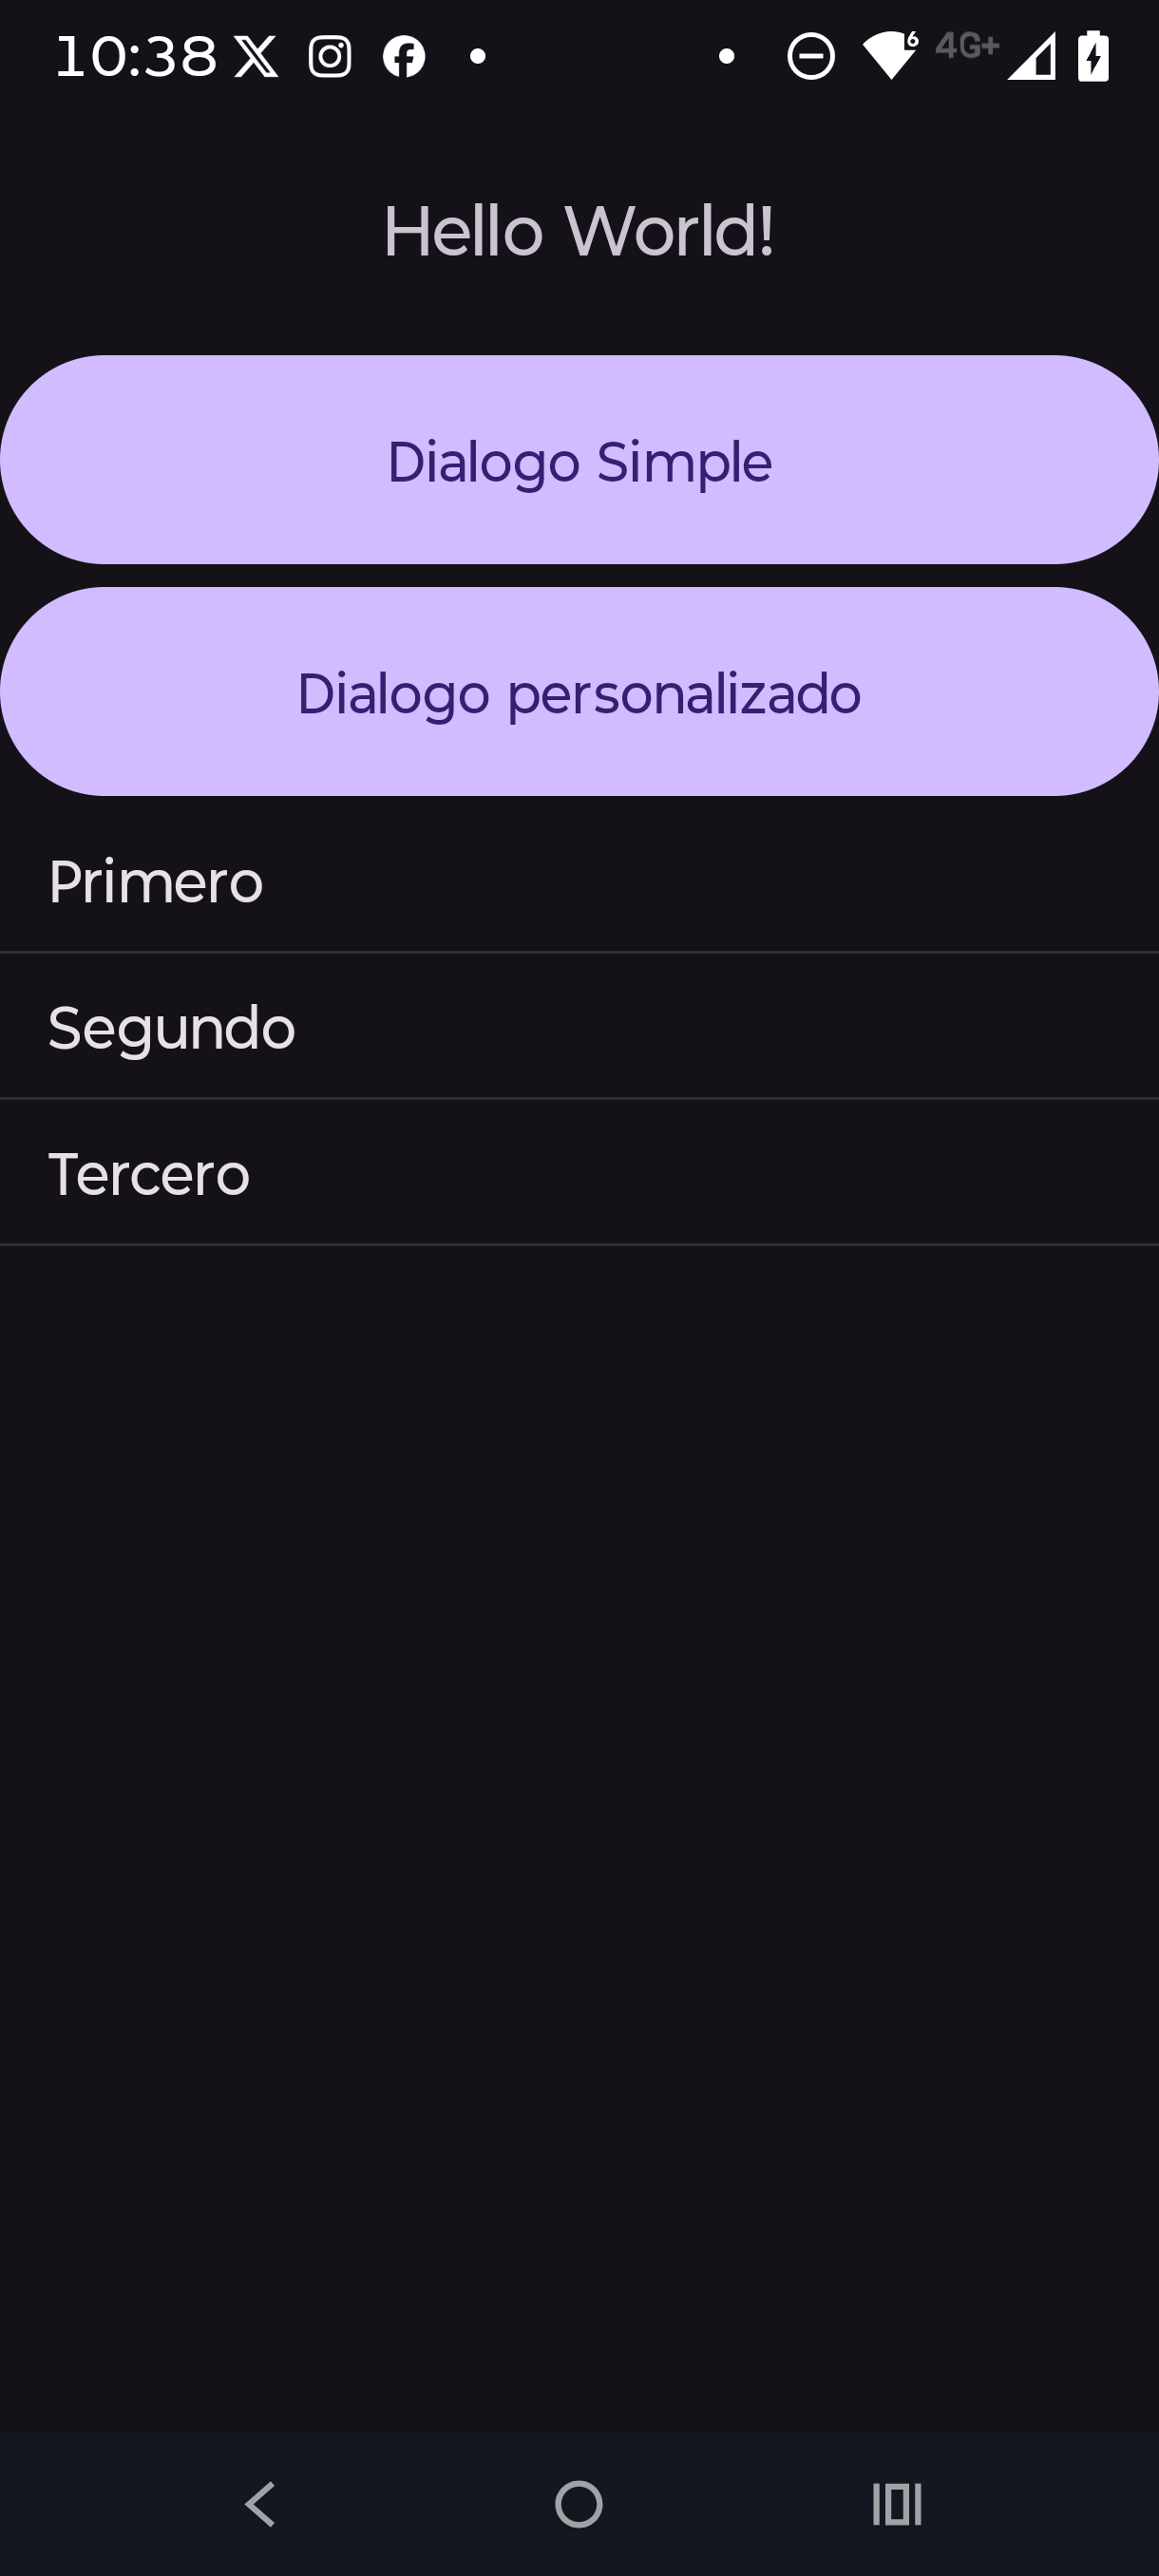
\includegraphics[width=0.98\textwidth]{02_TallerCBTis/figs/Demo11}
\end{center}

\end{columns}

\end{frame}


\begin{frame}[fragile]{Uso de TabHost y TabWidget en Android}
\textbf{¿Qué son TabHost y TabWidget?}

\begin{itemize}
    \item \textbf{TabHost:} Contenedor principal que gestiona múltiples pestañas (tabs).
    \item \textbf{TabWidget:} Componente visual que muestra las pestañas en la interfaz.
    \item Permiten organizar contenido en diferentes secciones dentro de una misma Activity.
\end{itemize}

\vspace{0.3cm}

\textbf{Estructura básica:}
\begin{itemize}
    \item TabHost contiene:
    \begin{itemize}
        \item Un \textbf{TabWidget} (las pestañas).
        \item Un \textbf{FrameLayout} (contenido de cada tab).
    \end{itemize}
\end{itemize}

\end{frame}


\begin{frame}[fragile]
\frametitle{Demo 12: Pestañas (Tabs)}
\begin{columns}
\column{0.80\linewidth}
Del Repositorio Github:
\begin{itemize}
\item Copiar el archivo \textit{MainActivity\_Demo12.java} (dentro del Folder códigosJAVA) al mismo directorio donde esta el MainActivity.java
\item Copiar el archivo \textit{activity\_main\_demo12.xml} (dentro del Folder Carpeta\_layout) al mismo directorio donde esta el activity\_main.xml
%\item Copiar el archivo \textit{custom\_dialog.xml} (dentro del Folder Carpeta\_layout) al mismo directorio donde esta el activity\_main.xml.
\item Modificar en el archivo \textit{AndroidManifest.xml} la cadena \textit{.MainActivity\_Demo11} por \textit{.MainActivity\_Demo12}.
%\item Ir a la linea 22 de archivo del archivo \textit{MainActivity\_Demo09.java}, poner el cursos en la palabra (en Rojo) \textit{documentfile}, presionar la combinación ALT+ENTER, y seleccionar de la lista desplegable la opcion ``Add dependency on ....''. Esto quitará el error y hara los ajustes necesarios. 
\end{itemize}

%\begin{block}{Demo \#09}
%Un App que permite escribir el contenido de un EditText a un archivo y cargar el contenido de cualquier archivo en el EditText
%\end{block}


\column{0.20\linewidth}

\begin{center}
 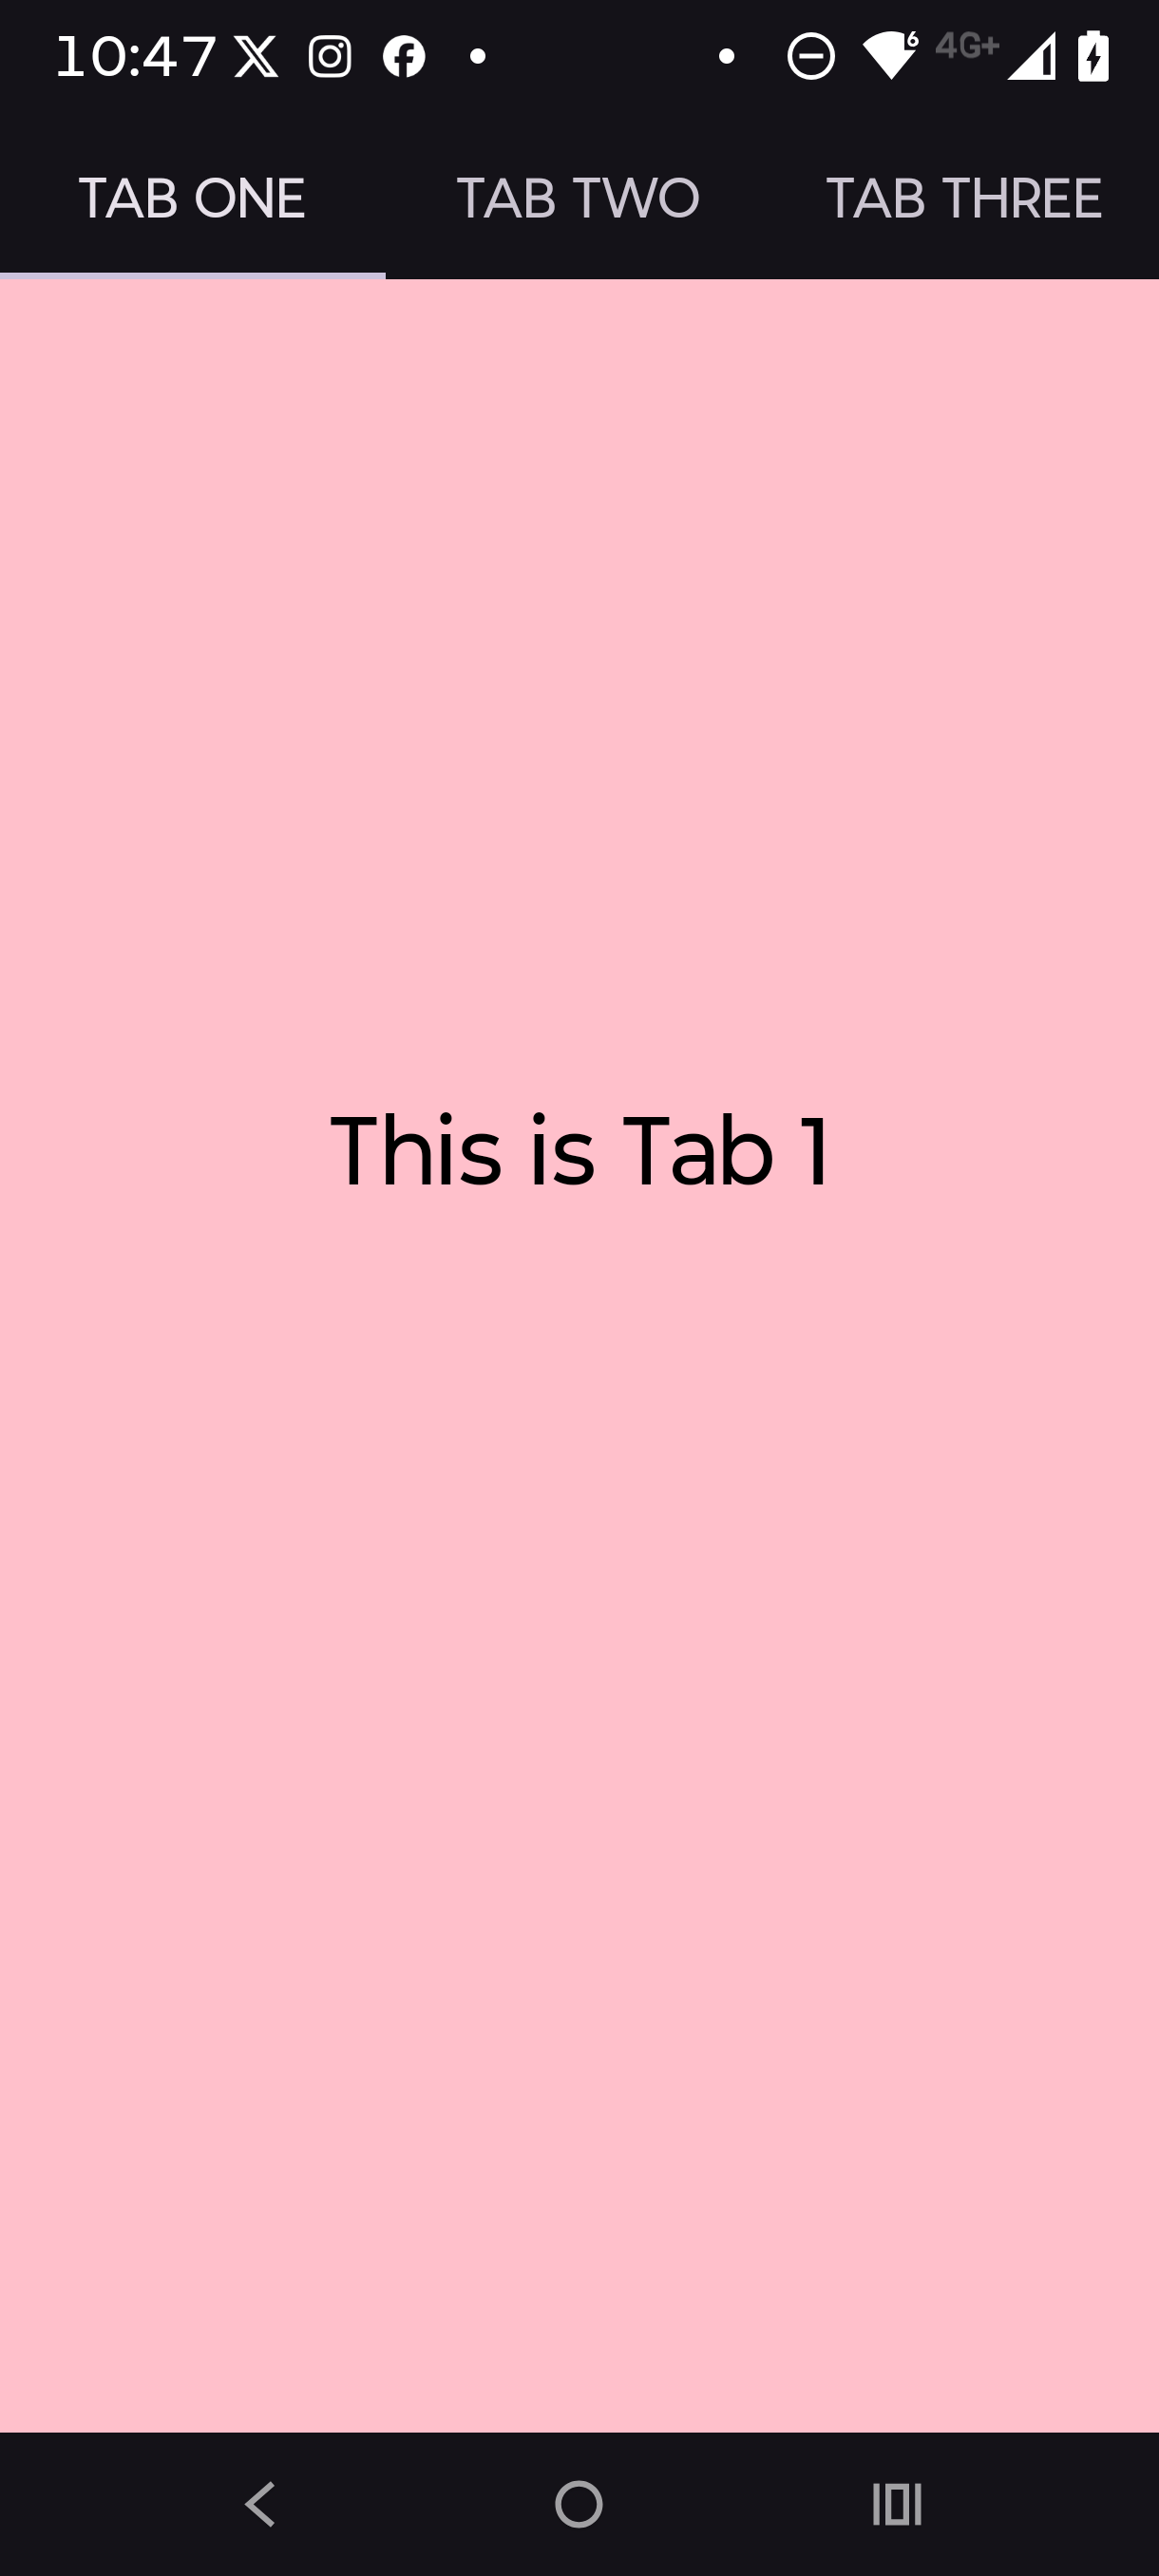
\includegraphics[width=0.98\textwidth]{02_TallerCBTis/figs/Demo12}
\end{center}

\end{columns}

\end{frame}



\begin{frame}[fragile]{Lectura de Códigos QR en Android}
\textbf{¿Qué es un decodificador QR?}

\begin{itemize}
    \item Permite leer y decodificar información contenida en códigos QR usando la cámara del dispositivo.
    \item Se utiliza en aplicaciones de pagos, accesos, inventarios, entre otros.
\end{itemize}

\textbf{Uso de librerías externas:}
\begin{itemize}
    \item Android no incluye un lector QR nativo completo.
    \item Se pueden integrar librerías como \textbf{ZXing} o \textbf{ML Kit}.

\scriptsize
\begin{minted}{groovy}
dependencies {
    implementation 'com.journeyapps:zxing-android-embedded:4.3.0'
    implementation 'com.google.zxing:core:3.5.1'
}
\end{minted}

\end{itemize}

\textbf{Ventajas:}
\begin{itemize}
    \item Integración rápida y sencilla.
    \item Soporte para múltiples formatos de códigos.
\end{itemize}

\end{frame}



\begin{frame}[fragile]
\frametitle{Demo 13: Decodificacion de Codigos QR con Camara }
\begin{columns}
\column{0.80\linewidth}
Del Repositorio Github:
\begin{itemize}
\item Copiar el archivo \textit{MainActivity\_Demo13.java} (dentro del Folder códigosJAVA) al mismo directorio donde esta el MainActivity.java
\item Copiar el archivo \textit{activity\_main\_demo13.xml} (dentro del Folder Carpeta\_layout) al mismo directorio donde esta el activity\_main.xml
%\item Copiar el archivo \textit{custom\_dialog.xml} (dentro del Folder Carpeta\_layout) al mismo directorio donde esta el activity\_main.xml.
\item Modificar en el archivo \textit{AndroidManifest.xml} la cadena \textit{.MainActivity\_Demo12} por \textit{.MainActivity\_Demo13}.
\item Agregar la siguiente linea: \textit{implementation (``com.journeyapps:zxing-android-embedded:4.3.0'')}, al final de la seccion Dependencies del archivo Build.graddle.kts (Module: App).

%\item Ir a la linea 22 de archivo del archivo \textit{MainActivity\_Demo09.java}, poner el cursos en la palabra (en Rojo) \textit{documentfile}, presionar la combinación ALT+ENTER, y seleccionar de la lista desplegable la opcion ``Add dependency on ....''. Esto quitará el error y hara los ajustes necesarios. 
\end{itemize}

%\begin{block}{Demo \#09}
%Un App que permite escribir el contenido de un EditText a un archivo y cargar el contenido de cualquier archivo en el EditText
%\end{block}


\column{0.20\linewidth}

\begin{center}
 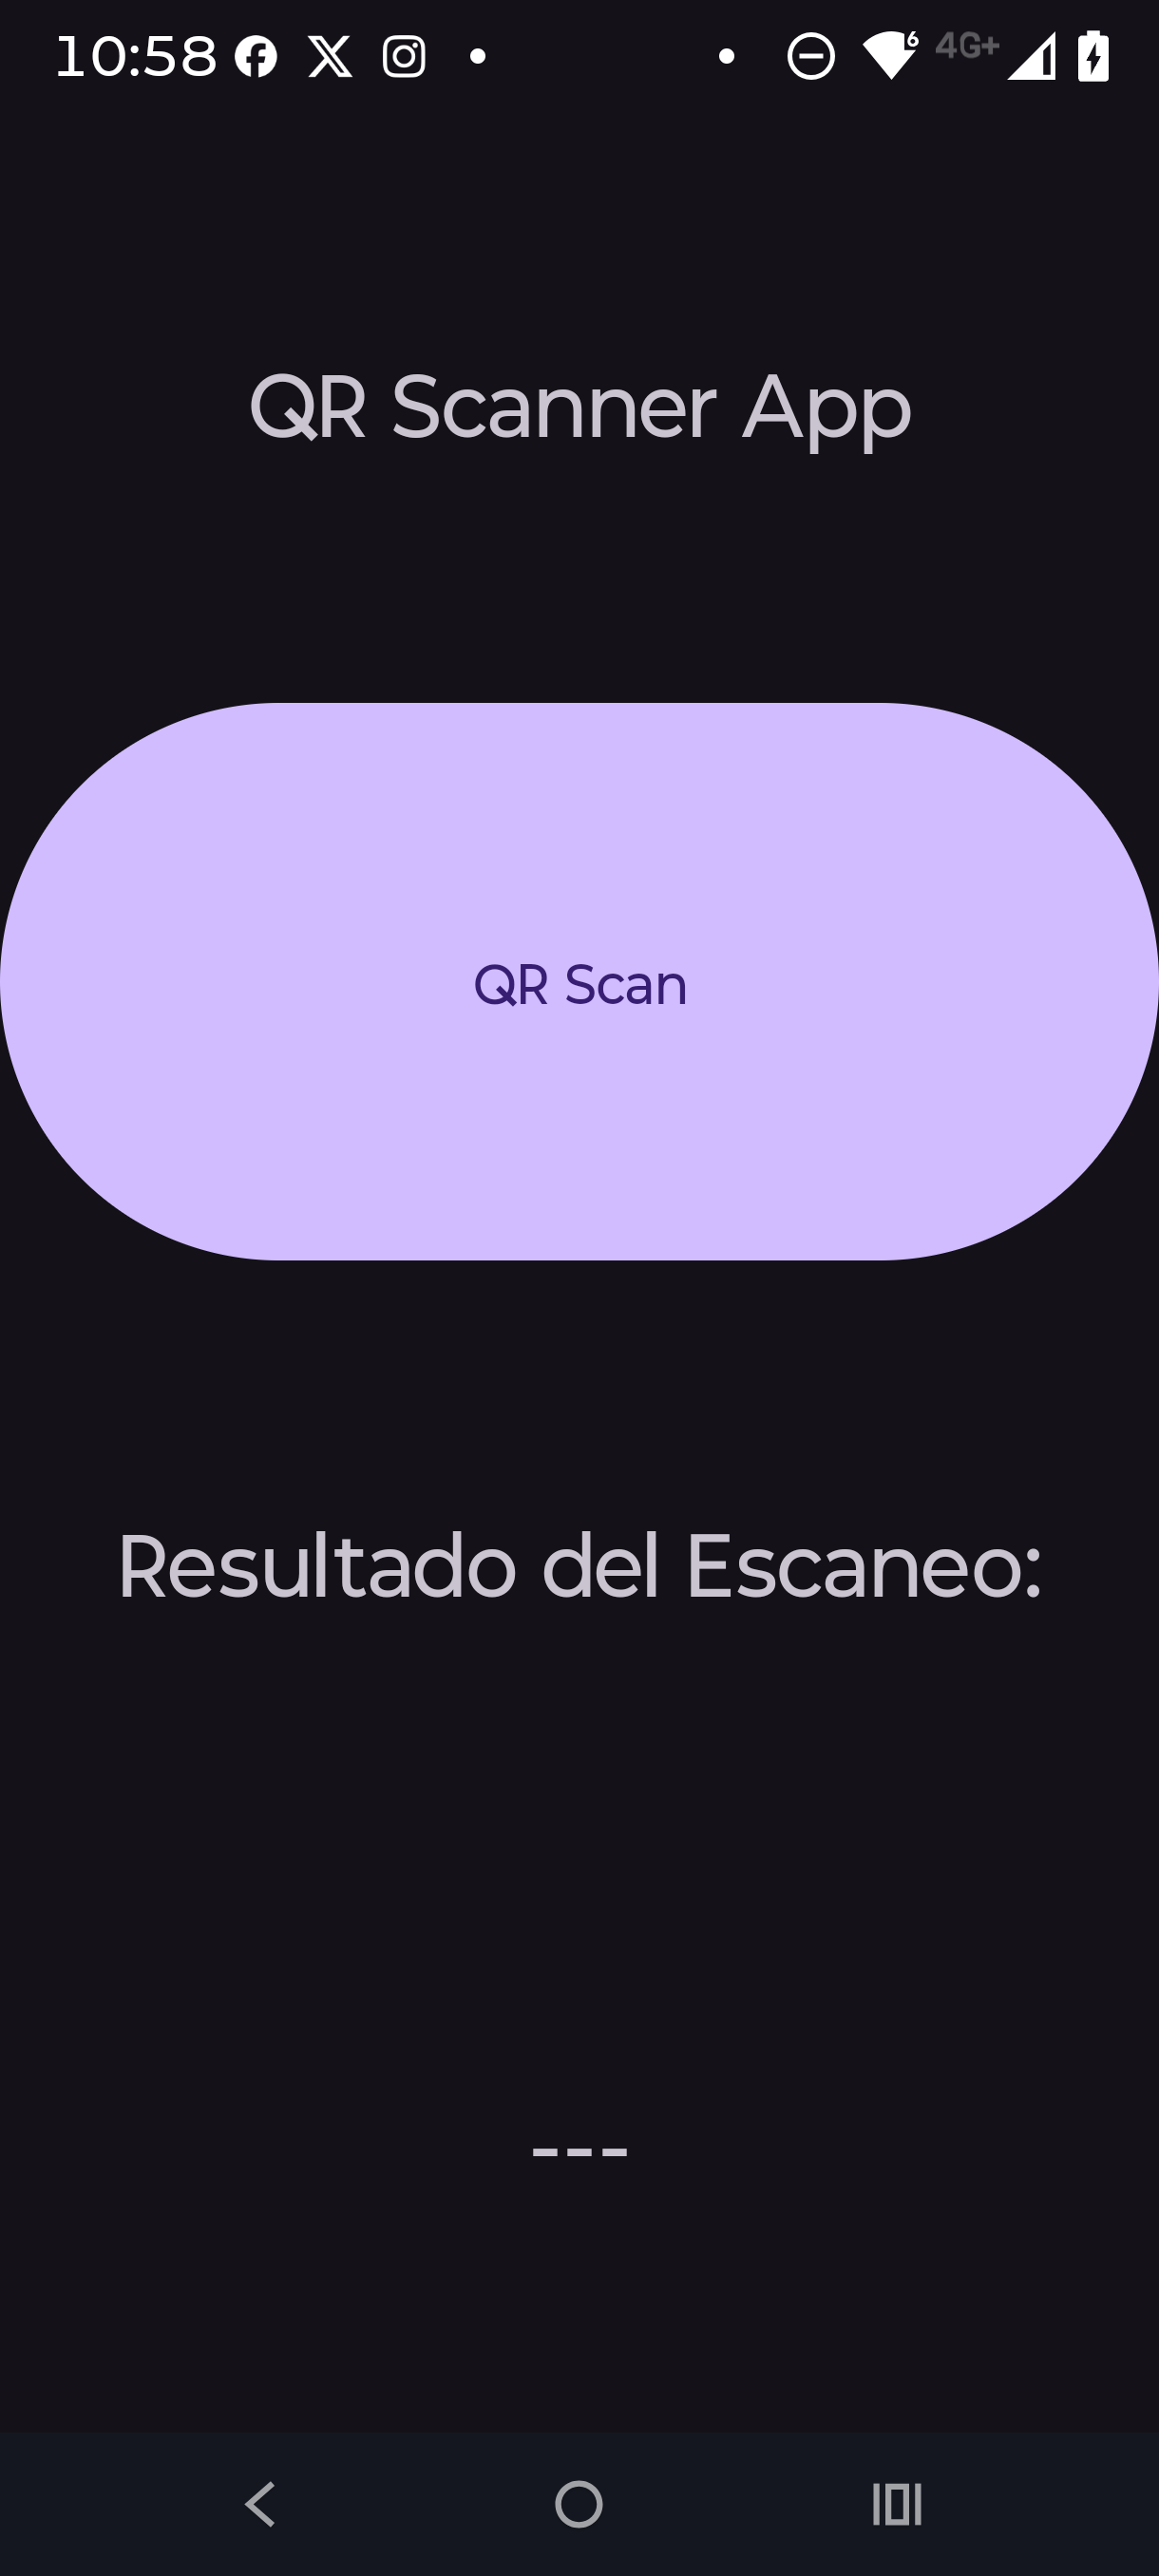
\includegraphics[width=0.98\textwidth]{02_TallerCBTis/figs/Demo13}
\end{center}

\end{columns}

\end{frame}


\begin{frame}[fragile]{Uso de Text-to-Speech (TTS) en Android}
\textbf{¿Qué es Text-to-Speech (TTS)?}

\begin{itemize}
    \item Es una tecnología que convierte texto en voz sintetizada.
    \item Permite a una aplicación "hablar" al usuario.
    \item Útil en accesibilidad, asistentes virtuales y notificaciones.
\end{itemize}


\textbf{Pasos básicos:}
\begin{itemize}
    \item Crear una instancia de \texttt{TextToSpeech}.
    \item Configurar idioma y velocidad.
    \item Invocar el método \texttt{speak()} para reproducir el texto.
\end{itemize}


\textbf{Consideraciones:}
\begin{itemize}
    \item Verificar que el idioma esté soportado.
    \item Liberar recursos con \texttt{tts.shutdown()} en \texttt{onDestroy()}.
    \item Requiere motor TTS instalado en el dispositivo.
\end{itemize}

\end{frame}



\begin{frame}[fragile]
\frametitle{Demo 14: Text to Speech (TTS) }
\begin{columns}
\column{0.80\linewidth}
Del Repositorio Github:
\begin{itemize}
\item Copiar el archivo \textit{MainActivity\_Demo14.java} (dentro del Folder códigosJAVA) al mismo directorio donde esta el MainActivity.java
\item Copiar el archivo \textit{activity\_main\_demo14.xml} (dentro del Folder Carpeta\_layout) al mismo directorio donde esta el activity\_main.xml
%\item Copiar el archivo \textit{custom\_dialog.xml} (dentro del Folder Carpeta\_layout) al mismo directorio donde esta el activity\_main.xml.
\item Modificar en el archivo \textit{AndroidManifest.xml} la cadena \textit{.MainActivity\_Demo13} por \textit{.MainActivity\_Demo14}.
%\item Agregar la siguiente linea: \textit{implementation (``com.journeyapps:zxing-android-embedded:4.3.0'')}, al final de la seccion Dependencies del archivo Build.graddle.kts (Module: App).

%\item Ir a la linea 22 de archivo del archivo \textit{MainActivity\_Demo09.java}, poner el cursos en la palabra (en Rojo) \textit{documentfile}, presionar la combinación ALT+ENTER, y seleccionar de la lista desplegable la opcion ``Add dependency on ....''. Esto quitará el error y hara los ajustes necesarios. 
\end{itemize}

%\begin{block}{Demo \#09}
%Un App que permite escribir el contenido de un EditText a un archivo y cargar el contenido de cualquier archivo en el EditText
%\end{block}


\column{0.20\linewidth}

\begin{center}
 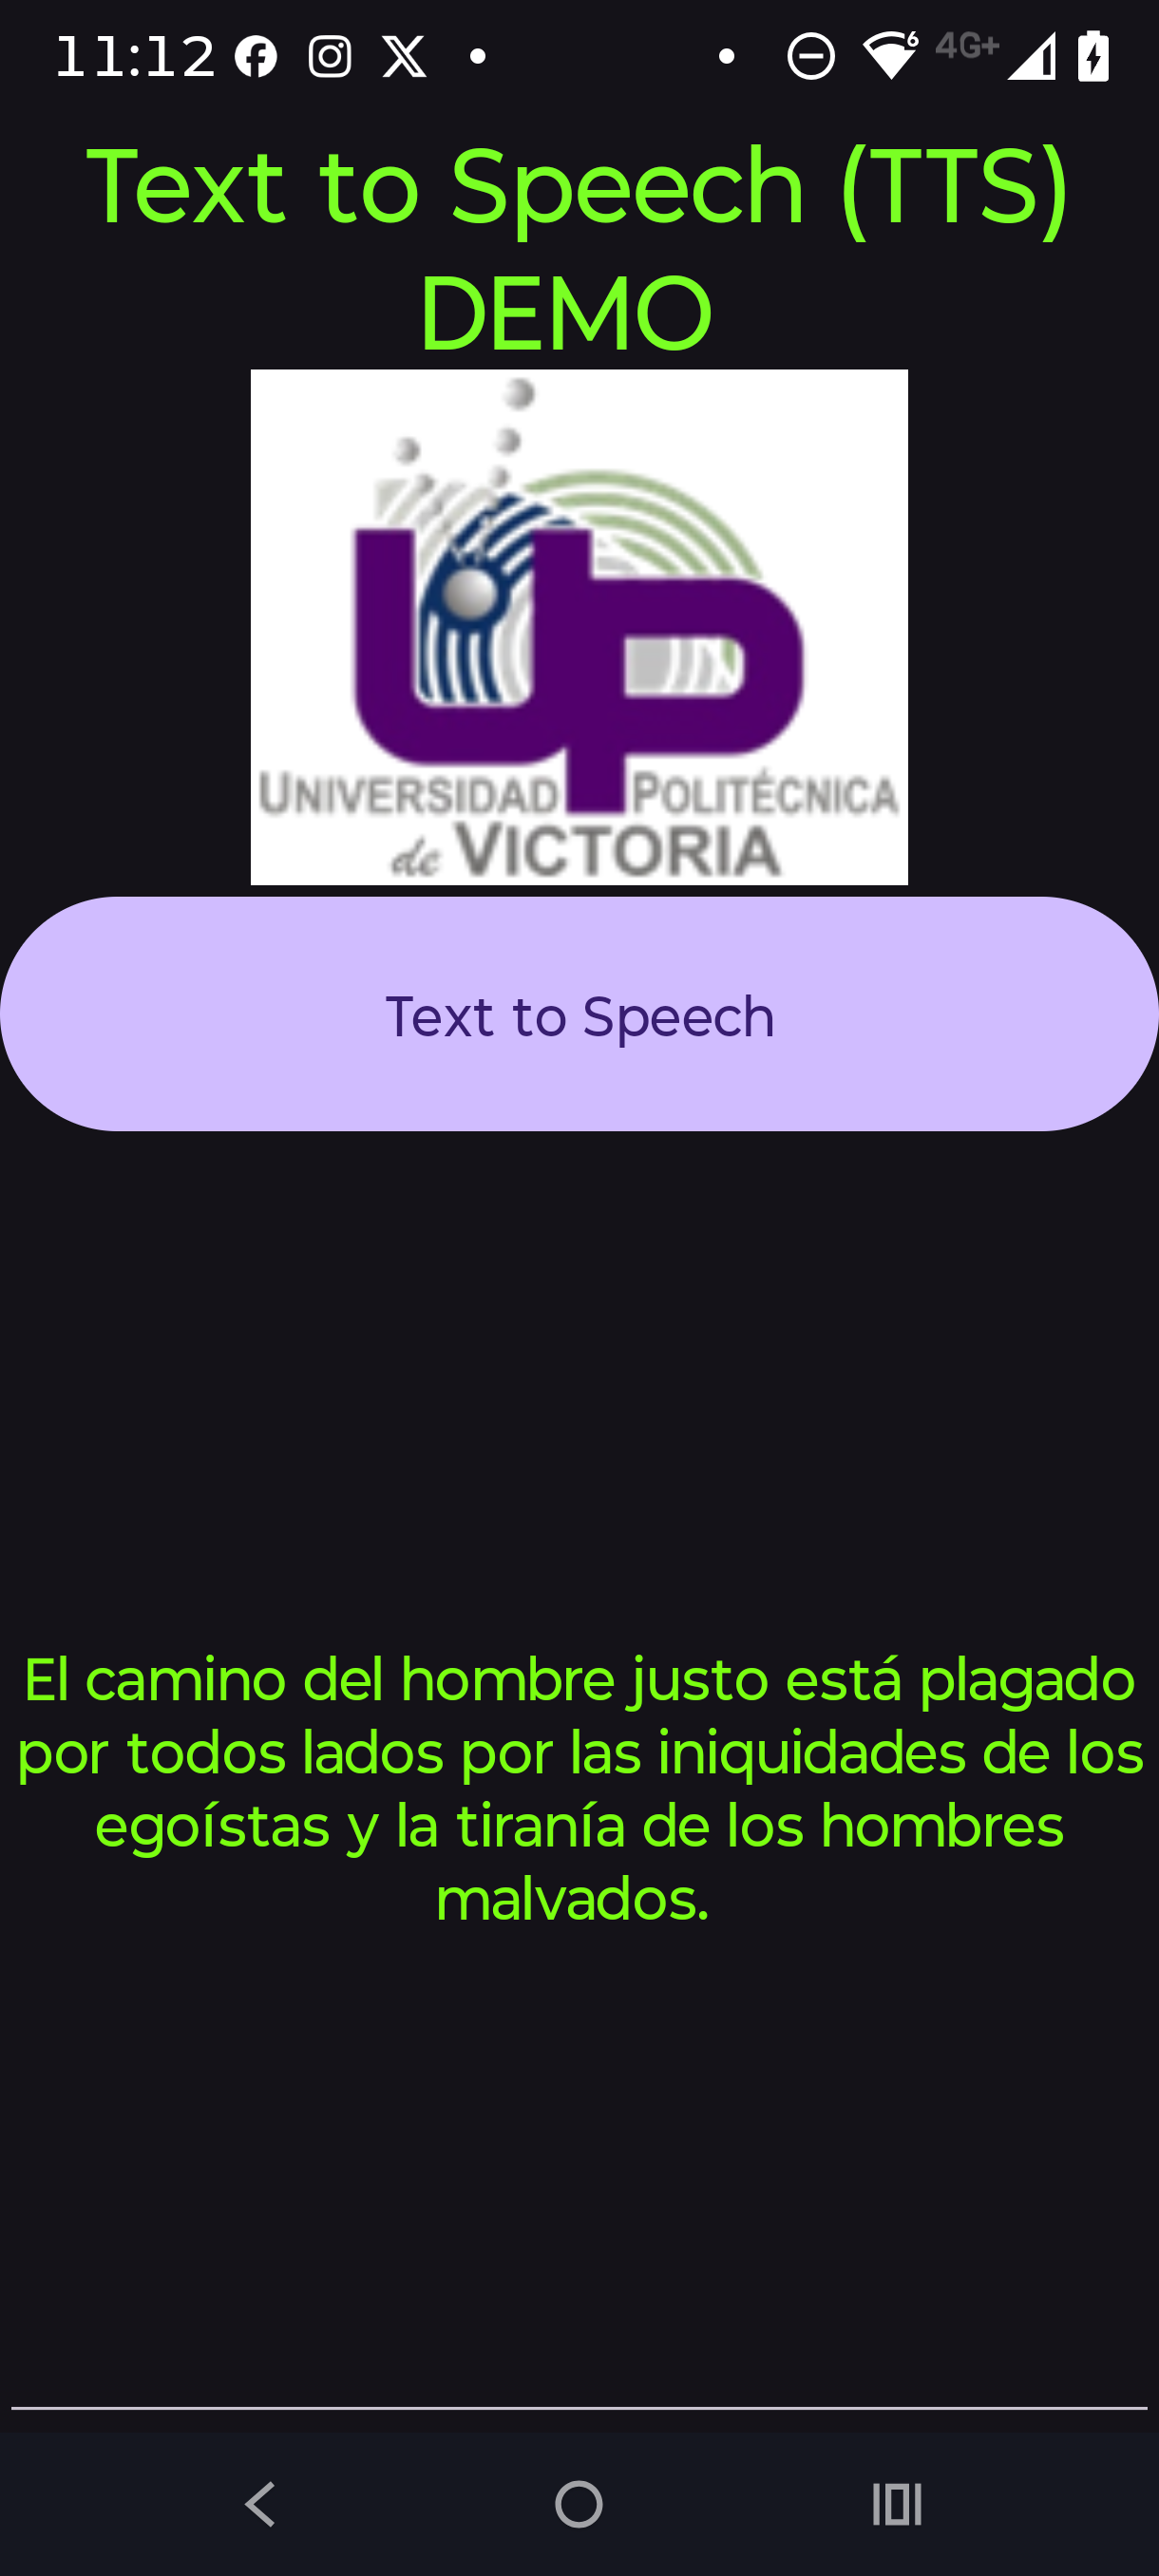
\includegraphics[width=0.98\textwidth]{02_TallerCBTis/figs/Demo14}
\end{center}

\end{columns}

\end{frame}



\begin{frame}[fragile]{Librería MPAndroidChart en Android}
\textbf{¿Qué es MPAndroidChart?}

\begin{itemize}
    \item Es una librería para la visualización de datos mediante gráficas en Android.
    \item Permite crear gráficos interactivos y altamente personalizables.
\end{itemize}

\vspace{0.3cm}

\textbf{Tipos de gráficas soportadas:}
\begin{itemize}
    \item Gráficas de línea (LineChart)
    \item Barras (BarChart)
    \item Pastel (PieChart)
    \item Dispersión (ScatterChart)
\end{itemize}

\textbf{Ventajas:}
\begin{itemize}
    \item Fácil integración.
    \item Alta personalización (colores, animaciones).
    \item Soporte para interacción (zoom, desplazamiento).
\end{itemize}

\end{frame}



\begin{frame}[fragile]
\frametitle{Demo 15: Graficas con MPAndroid  }
\begin{columns}
\column{0.80\linewidth}

\scriptsize
Del Repositorio Github:
\begin{itemize}
\item Agregar la siguiente linea: \textit{implementation("com.github.PhilJay:MPAndroidChart:v3.1.0")}, al final de la seccion Dependencies del archivo Build.graddle.kts (Module: App).
\item Agregar la siguiente linea: \textit{maven \{ url = uri(``https://jitpack.io'') \}}, al final de la seccion \textit{dependencyResolutionManagement } del archivo settings.graddle.kts.
\item Copiar el archivo \textit{MainActivity\_Demo15.java} (dentro del Folder códigosJAVA) al mismo directorio donde esta el MainActivity.java
\item Copiar el archivo \textit{activity\_main\_demo15.xml} (dentro del Folder Carpeta\_layout) al mismo directorio donde esta el activity\_main.xml
\item Modificar en el archivo \textit{AndroidManifest.xml} la cadena \textit{.MainActivity\_Demo14} por \textit{.MainActivity\_Demo15}.

%\item Ir a la linea 22 de archivo del archivo \textit{MainActivity\_Demo09.java}, poner el cursos en la palabra (en Rojo) \textit{documentfile}, presionar la combinación ALT+ENTER, y seleccionar de la lista desplegable la opcion ``Add dependency on ....''. Esto quitará el error y hara los ajustes necesarios. 
\end{itemize}

%\begin{block}{Demo \#09}
%Un App que permite escribir el contenido de un EditText a un archivo y cargar el contenido de cualquier archivo en el EditText
%\end{block}


\column{0.20\linewidth}

\begin{center}
 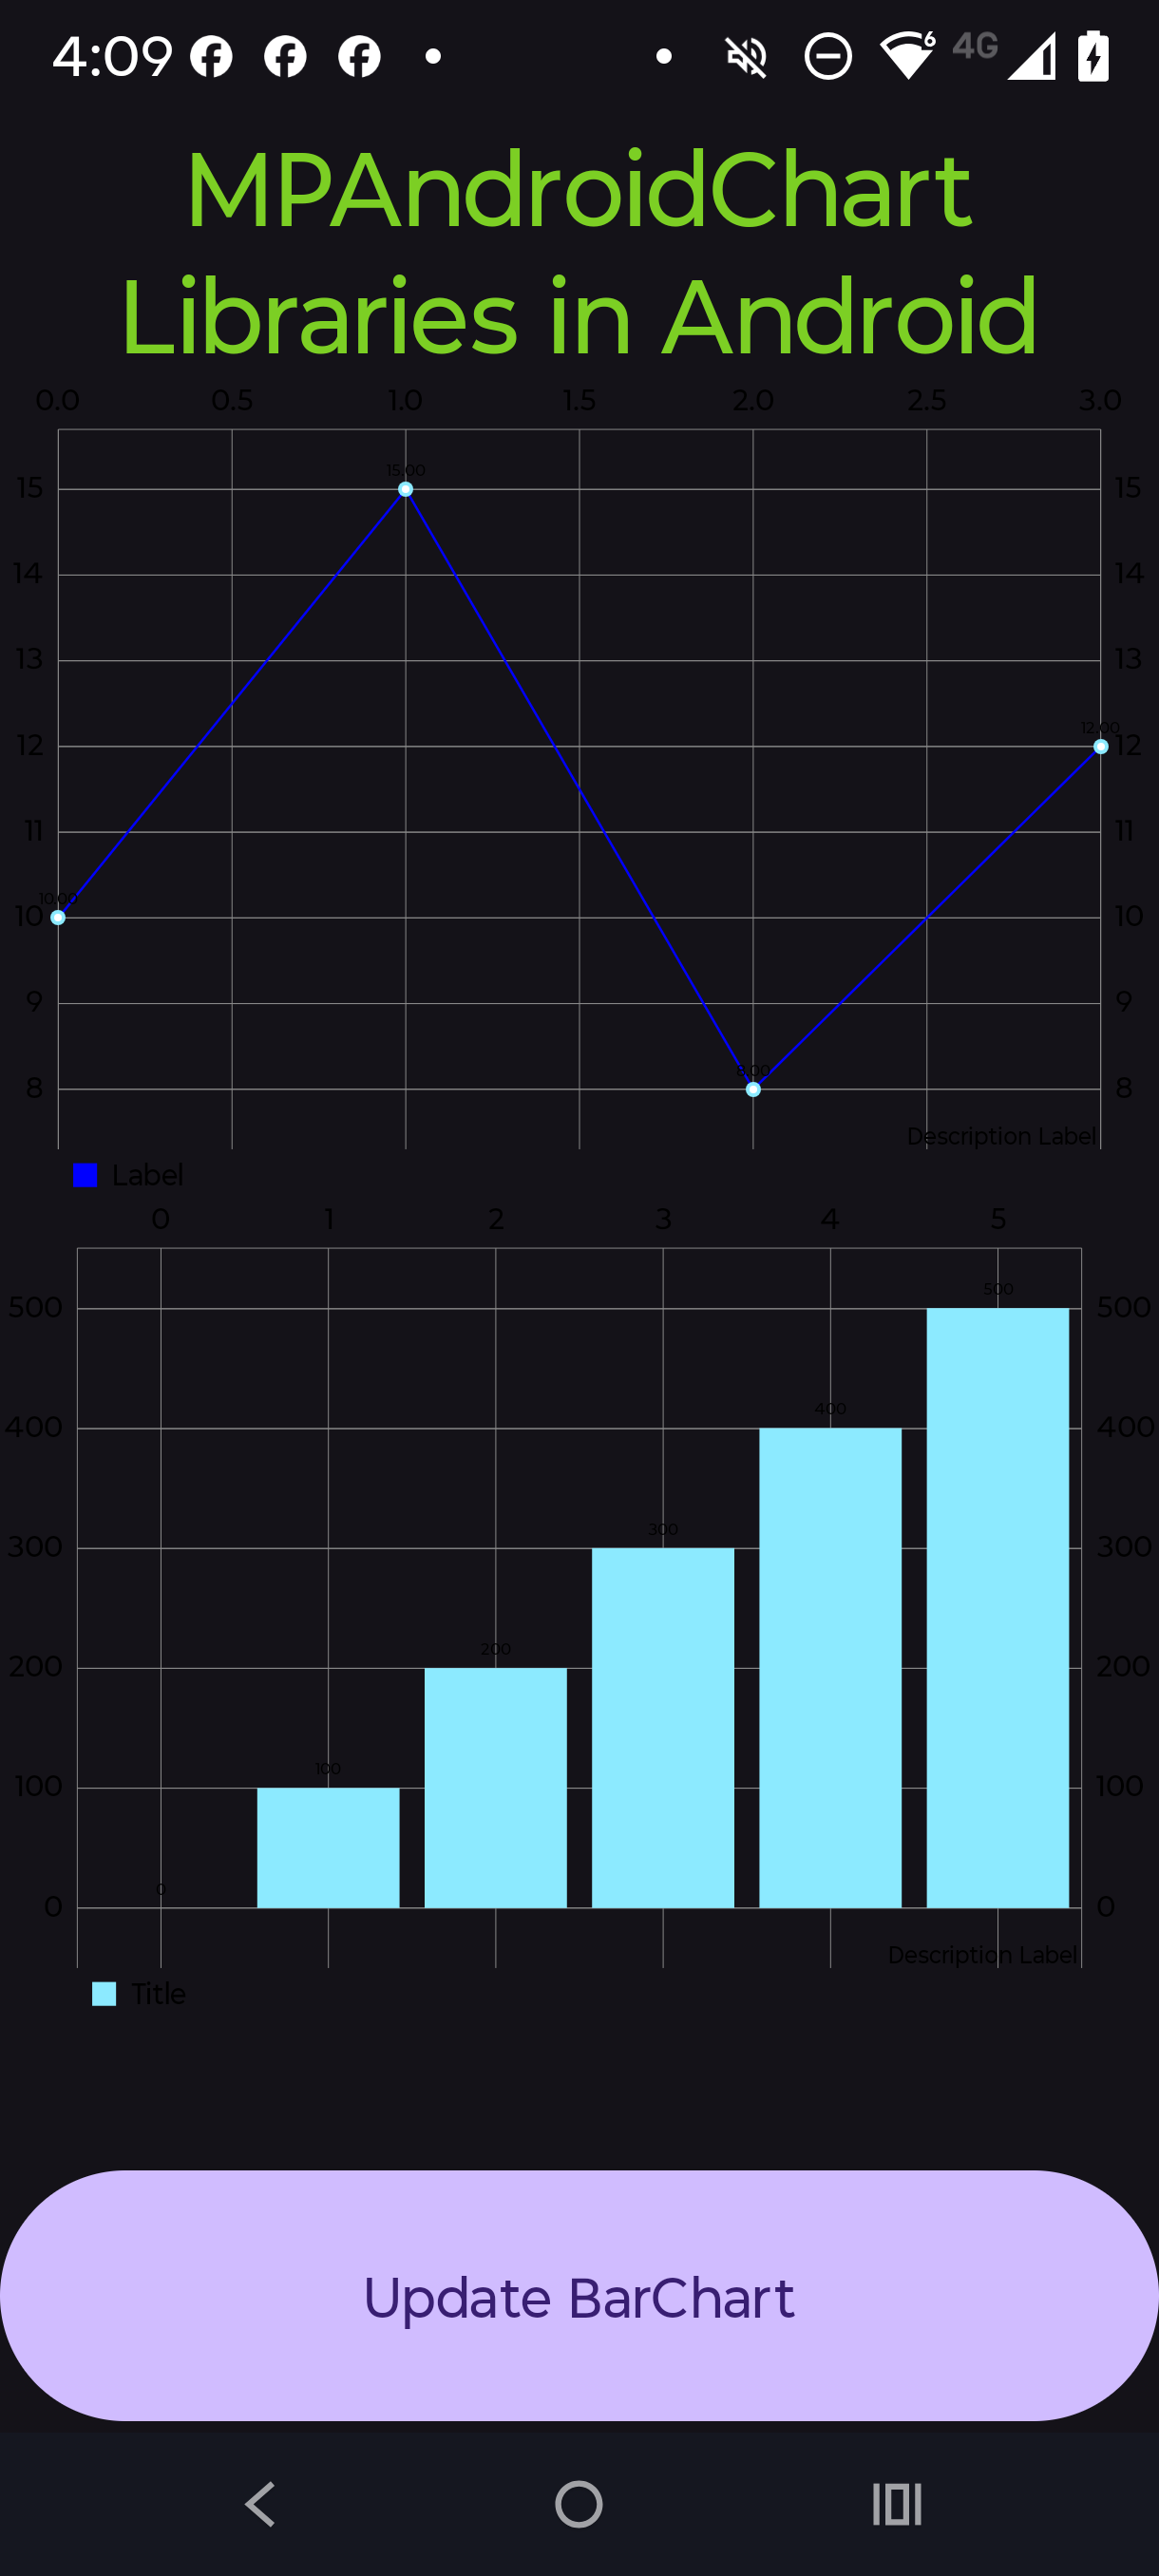
\includegraphics[width=0.98\textwidth]{02_TallerCBTis/figs/Demo15}
\end{center}

\end{columns}

\end{frame}


\begin{frame}[fragile]{Uso de Canvas View en Android}
\textbf{¿Qué es un Canvas View?}

\begin{itemize}
    \item Permite dibujar gráficos personalizados directamente en pantalla.
    \item Se utiliza extendiendo la clase \texttt{View} y sobrescribiendo el método \texttt{onDraw()}.
    \item Ideal para juegos, visualizaciones y dibujo libre.
\end{itemize}


\textbf{Métodos principales:}
\begin{itemize}
    \item \textbf{onDraw(Canvas canvas):} Método donde se realiza el dibujo.
    \item \textbf{invalidate():} Solicita redibujar la vista.
    \item \textbf{onTouchEvent():} Maneja interacción táctil.
\end{itemize}


\textbf{Clases importantes:}
\begin{itemize}
    \item \textbf{Canvas:} Superficie de dibujo.
    \item \textbf{Paint:} Define color, estilo y grosor.
    \item \textbf{Path:} Permite dibujar formas complejas.
\end{itemize}


\textbf{Ventajas:}
\begin{itemize}
    \item Alto control sobre gráficos.
    \item Ideal para interfaces personalizadas.
\end{itemize}

\end{frame}



\begin{frame}[fragile]
\frametitle{Demo 16: CanvasView }
\begin{columns}
\column{0.80\linewidth}

\scriptsize
Del Repositorio Github:
\begin{itemize}
%\item Agregar la siguiente linea: \textit{implementation("com.github.PhilJay:MPAndroidChart:v3.1.0")}, al final de la seccion Dependencies del archivo Build.graddle.kts (Module: App).
%\item Agregar la siguiente linea: \textit{maven \{ url = uri(``https://jitpack.io'') \}}, al final de la seccion \textit{dependencyResolutionManagement } del archivo settings.graddle.kts.
\item Copiar el archivo \textit{MainActivity\_Demo16.java} (dentro del Folder códigosJAVA) al mismo directorio donde esta el MainActivity.java
\item Copiar el archivo \textit{CanvasView.java} (dentro del Folder códigosJAVA) al mismo directorio donde esta el MainActivity.java

\item Copiar el archivo \textit{activity\_main\_demo16.xml} (dentro del Folder Carpeta\_layout) al mismo directorio donde esta el activity\_main.xml
\item Modificar dentro del archivo \textit{activity\_main\_demo16.xml} la cadena \textit{.com.example.a2026\_01\_holamundoandroid.CanvasView} por \textit{$<$SuPackage$>$.CanvasView}.
\item Modificar en el archivo \textit{AndroidManifest.xml} la cadena \textit{.MainActivity\_Demo15} por \textit{.MainActivity\_Demo16}.


%\item Ir a la linea 22 de archivo del archivo \textit{MainActivity\_Demo09.java}, poner el cursos en la palabra (en Rojo) \textit{documentfile}, presionar la combinación ALT+ENTER, y seleccionar de la lista desplegable la opcion ``Add dependency on ....''. Esto quitará el error y hara los ajustes necesarios. 
\end{itemize}

%\begin{block}{Demo \#09}
%Un App que permite escribir el contenido de un EditText a un archivo y cargar el contenido de cualquier archivo en el EditText
%\end{block}


\column{0.20\linewidth}

\begin{center}
 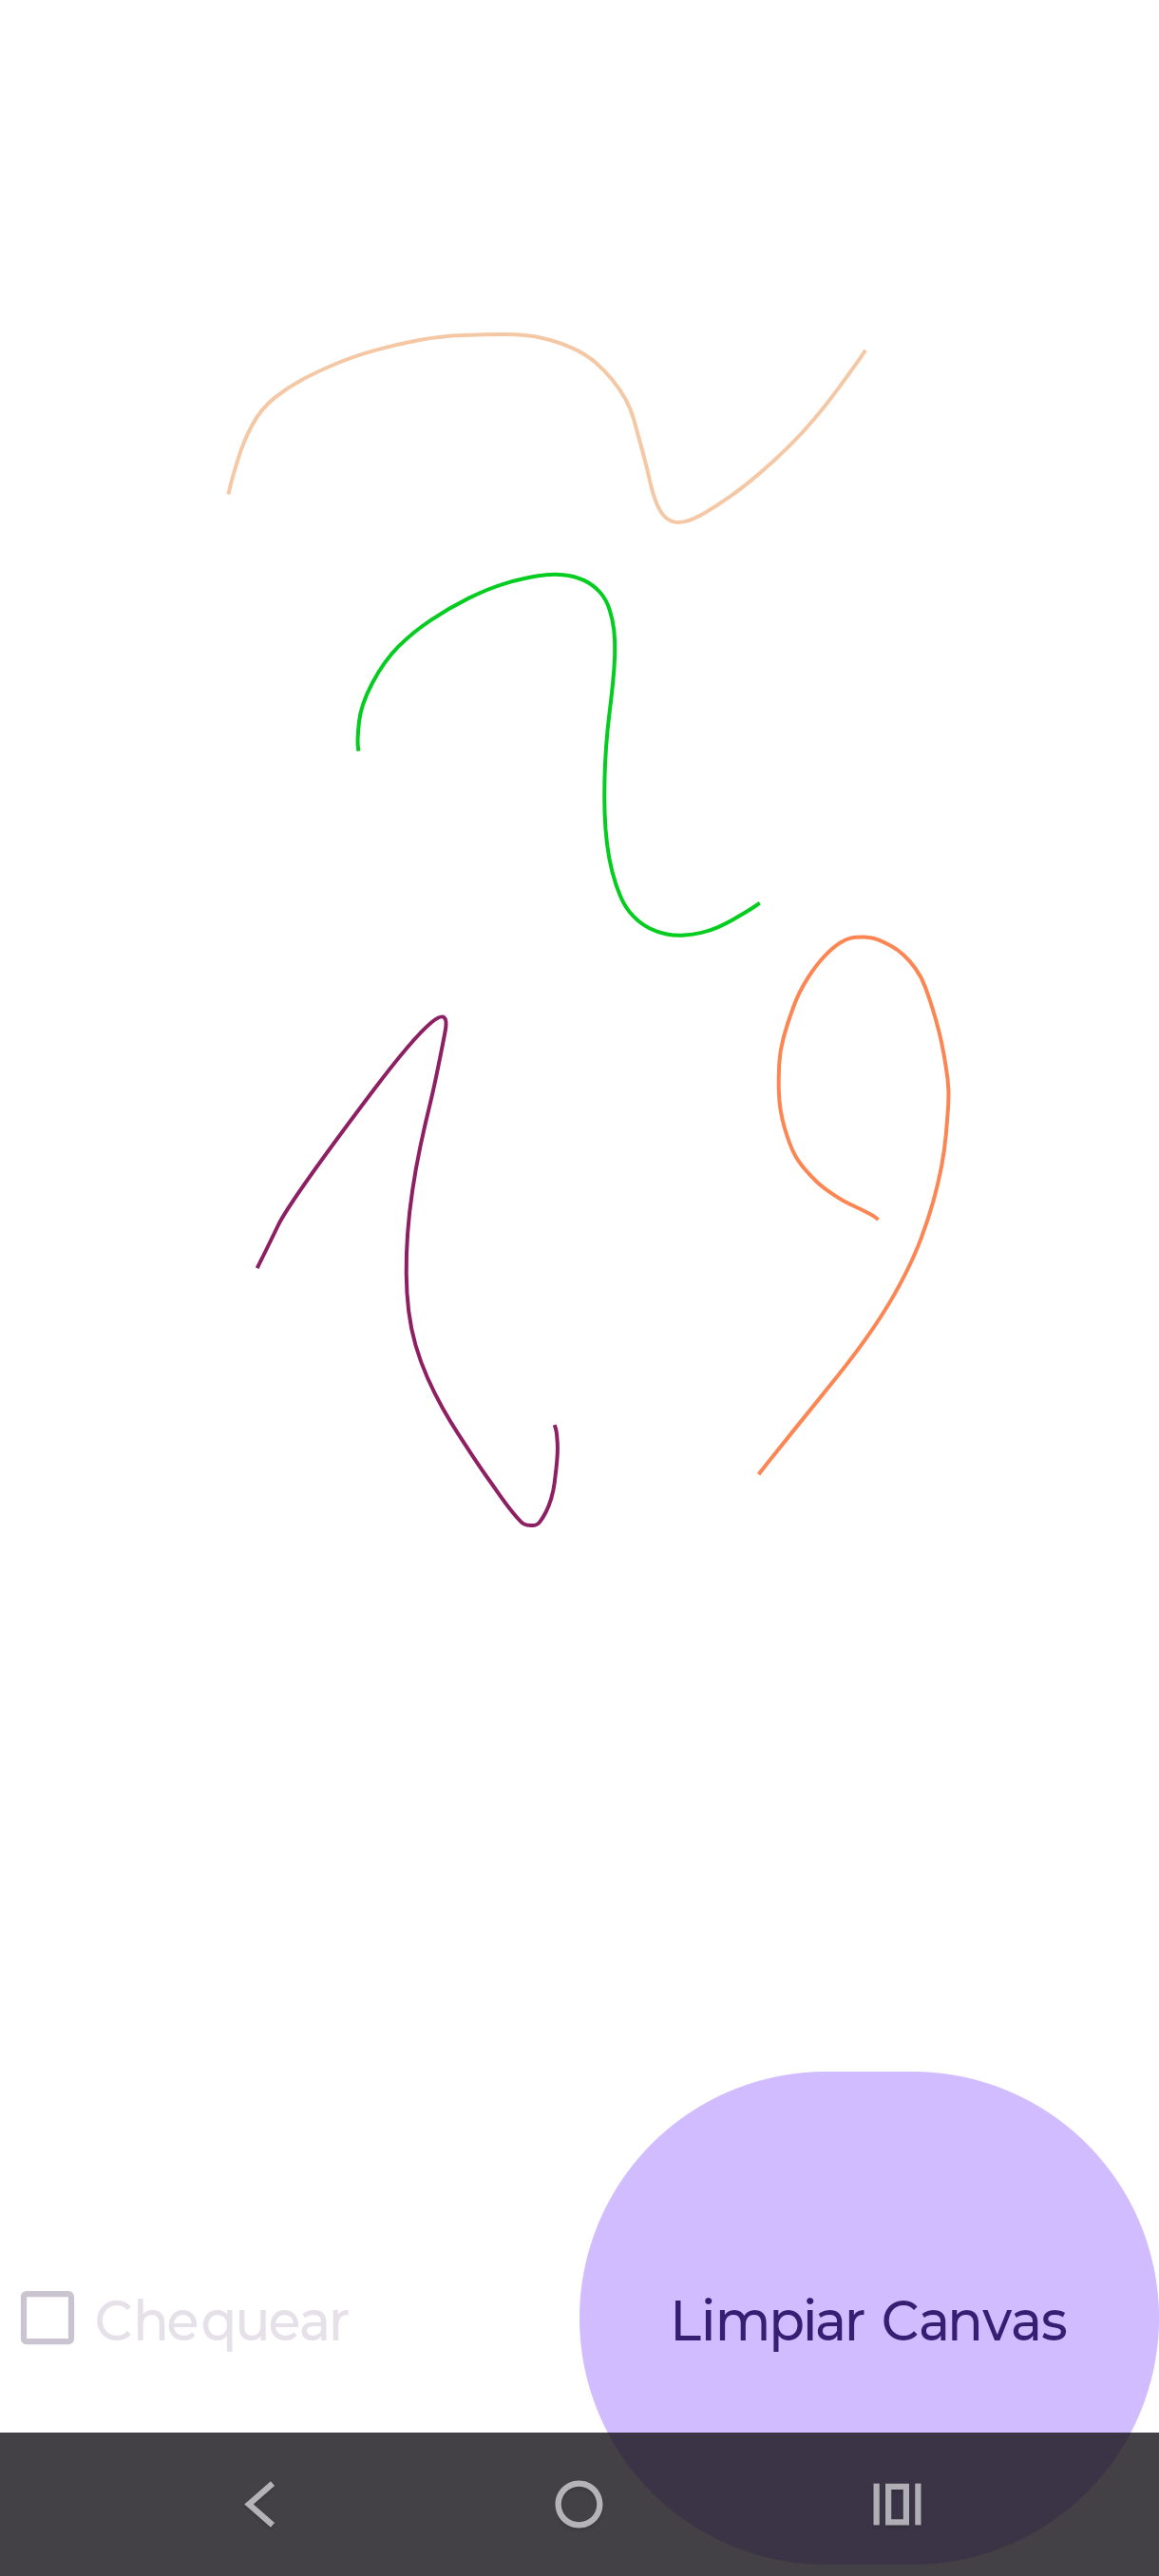
\includegraphics[width=0.98\textwidth]{02_TallerCBTis/figs/Demo16}
\end{center}

\end{columns}

\end{frame}


\begin{frame}[fragile]{Uso de SurfaceView en Android}
\textbf{¿Qué es SurfaceView?}

\begin{itemize}
    \item Es un componente que permite dibujar directamente sobre una superficie separada del hilo principal (UI thread).
    \item Ideal para gráficos en tiempo real como videojuegos, animaciones o streaming de video.
\end{itemize}

\textbf{Componentes clave:}
\begin{itemize}
    \item \textbf{SurfaceHolder:} Controla la superficie de dibujo.
    \item \textbf{Canvas:} Permite realizar los dibujos.
    \item \textbf{Thread:} Maneja el ciclo de renderizado.
\end{itemize}

\textbf{Métodos principales (SurfaceHolder.Callback):}
\begin{itemize}
    \item \textbf{surfaceCreated():} Se invoca cuando la superficie está lista para dibujar.
    \item \textbf{surfaceChanged():} Se ejecuta cuando cambia tamaño o formato.
    \item \textbf{surfaceDestroyed():} Se llama cuando la superficie se destruye.
\end{itemize}

\textbf{Ventajas:}
\begin{itemize}
    \item Alto rendimiento para gráficos.
    \item Control directo del renderizado.
\end{itemize}

\end{frame}




\begin{frame}[fragile]{Drag and Drop y SurfaceView en Android}
\textbf{¿Qué es Drag and Drop?}

\begin{itemize}
    \item Es una técnica de interacción que permite arrastrar (drag) y soltar (drop) elementos en la pantalla.
\end{itemize}

\textbf{Implementación en Android:}
\begin{itemize}
    \item Uso de eventos táctiles (\texttt{onTouchEvent}).
    \item Manejo de coordenadas (X, Y) para actualizar la posición del objeto.
    \item Uso de \texttt{setOnDragListener()} en vistas estándar.
\end{itemize}

\vspace{0.3cm}

\textbf{Relación con SurfaceView:}
\begin{itemize}
    \item En \textbf{SurfaceView} el control es manual:
    \begin{itemize}
        \item Se capturan eventos táctiles.
        \item Se redibuja el objeto en nuevas posiciones usando \texttt{Canvas}.
    \end{itemize}
\end{itemize}


\textbf{Ventajas:}
\begin{itemize}
    \item Ideal para juegos o interfaces dinámicas. Permite interacción intuitiva y mayor control en SurfaceView para animaciones en tiempo real.
\end{itemize}

\end{frame}




\begin{frame}[fragile]
\frametitle{Demo 17: Surface View }
\begin{columns}
\column{0.80\linewidth}

\scriptsize
Del Repositorio Github:
\begin{itemize}
%\item Agregar la siguiente linea: \textit{implementation("com.github.PhilJay:MPAndroidChart:v3.1.0")}, al final de la seccion Dependencies del archivo Build.graddle.kts (Module: App).
%\item Agregar la siguiente linea: \textit{maven \{ url = uri(``https://jitpack.io'') \}}, al final de la seccion \textit{dependencyResolutionManagement } del archivo settings.graddle.kts.
\item Copiar el archivo \textit{MainActivity\_Demo17.java} (dentro del Folder códigosJAVA) al mismo directorio donde esta el MainActivity.java
\item Copiar los archivos \textit{DragAndDropView.java, DragAndDropThread.java, Circulo.java, Figura.java y Rectangulo.java},  (dentro del Folder códigosJAVA) al mismo directorio donde esta el MainActivity.java
\item Copiar el archivo \textit{activity\_main\_demo17.xml} (dentro del Folder Carpeta\_layout) al mismo directorio donde esta el activity\_main.xml
\item Modificar dentro del archivo \textit{activity\_main\_demo17.xml} la cadena \textit{.com.example.a2026\_01\_holamundoandroid.DragAndDropView} por \textit{$<$SuPackage$>$.DragAndDropView}.
\item Modificar en el archivo \textit{AndroidManifest.xml} la cadena \textit{.MainActivity\_Demo16} por \textit{.MainActivity\_Demo17}.


%\item Ir a la linea 22 de archivo del archivo \textit{MainActivity\_Demo09.java}, poner el cursos en la palabra (en Rojo) \textit{documentfile}, presionar la combinación ALT+ENTER, y seleccionar de la lista desplegable la opcion ``Add dependency on ....''. Esto quitará el error y hara los ajustes necesarios. 
\end{itemize}

%\begin{block}{Demo \#09}
%Un App que permite escribir el contenido de un EditText a un archivo y cargar el contenido de cualquier archivo en el EditText
%\end{block}


\column{0.20\linewidth}

\begin{center}
 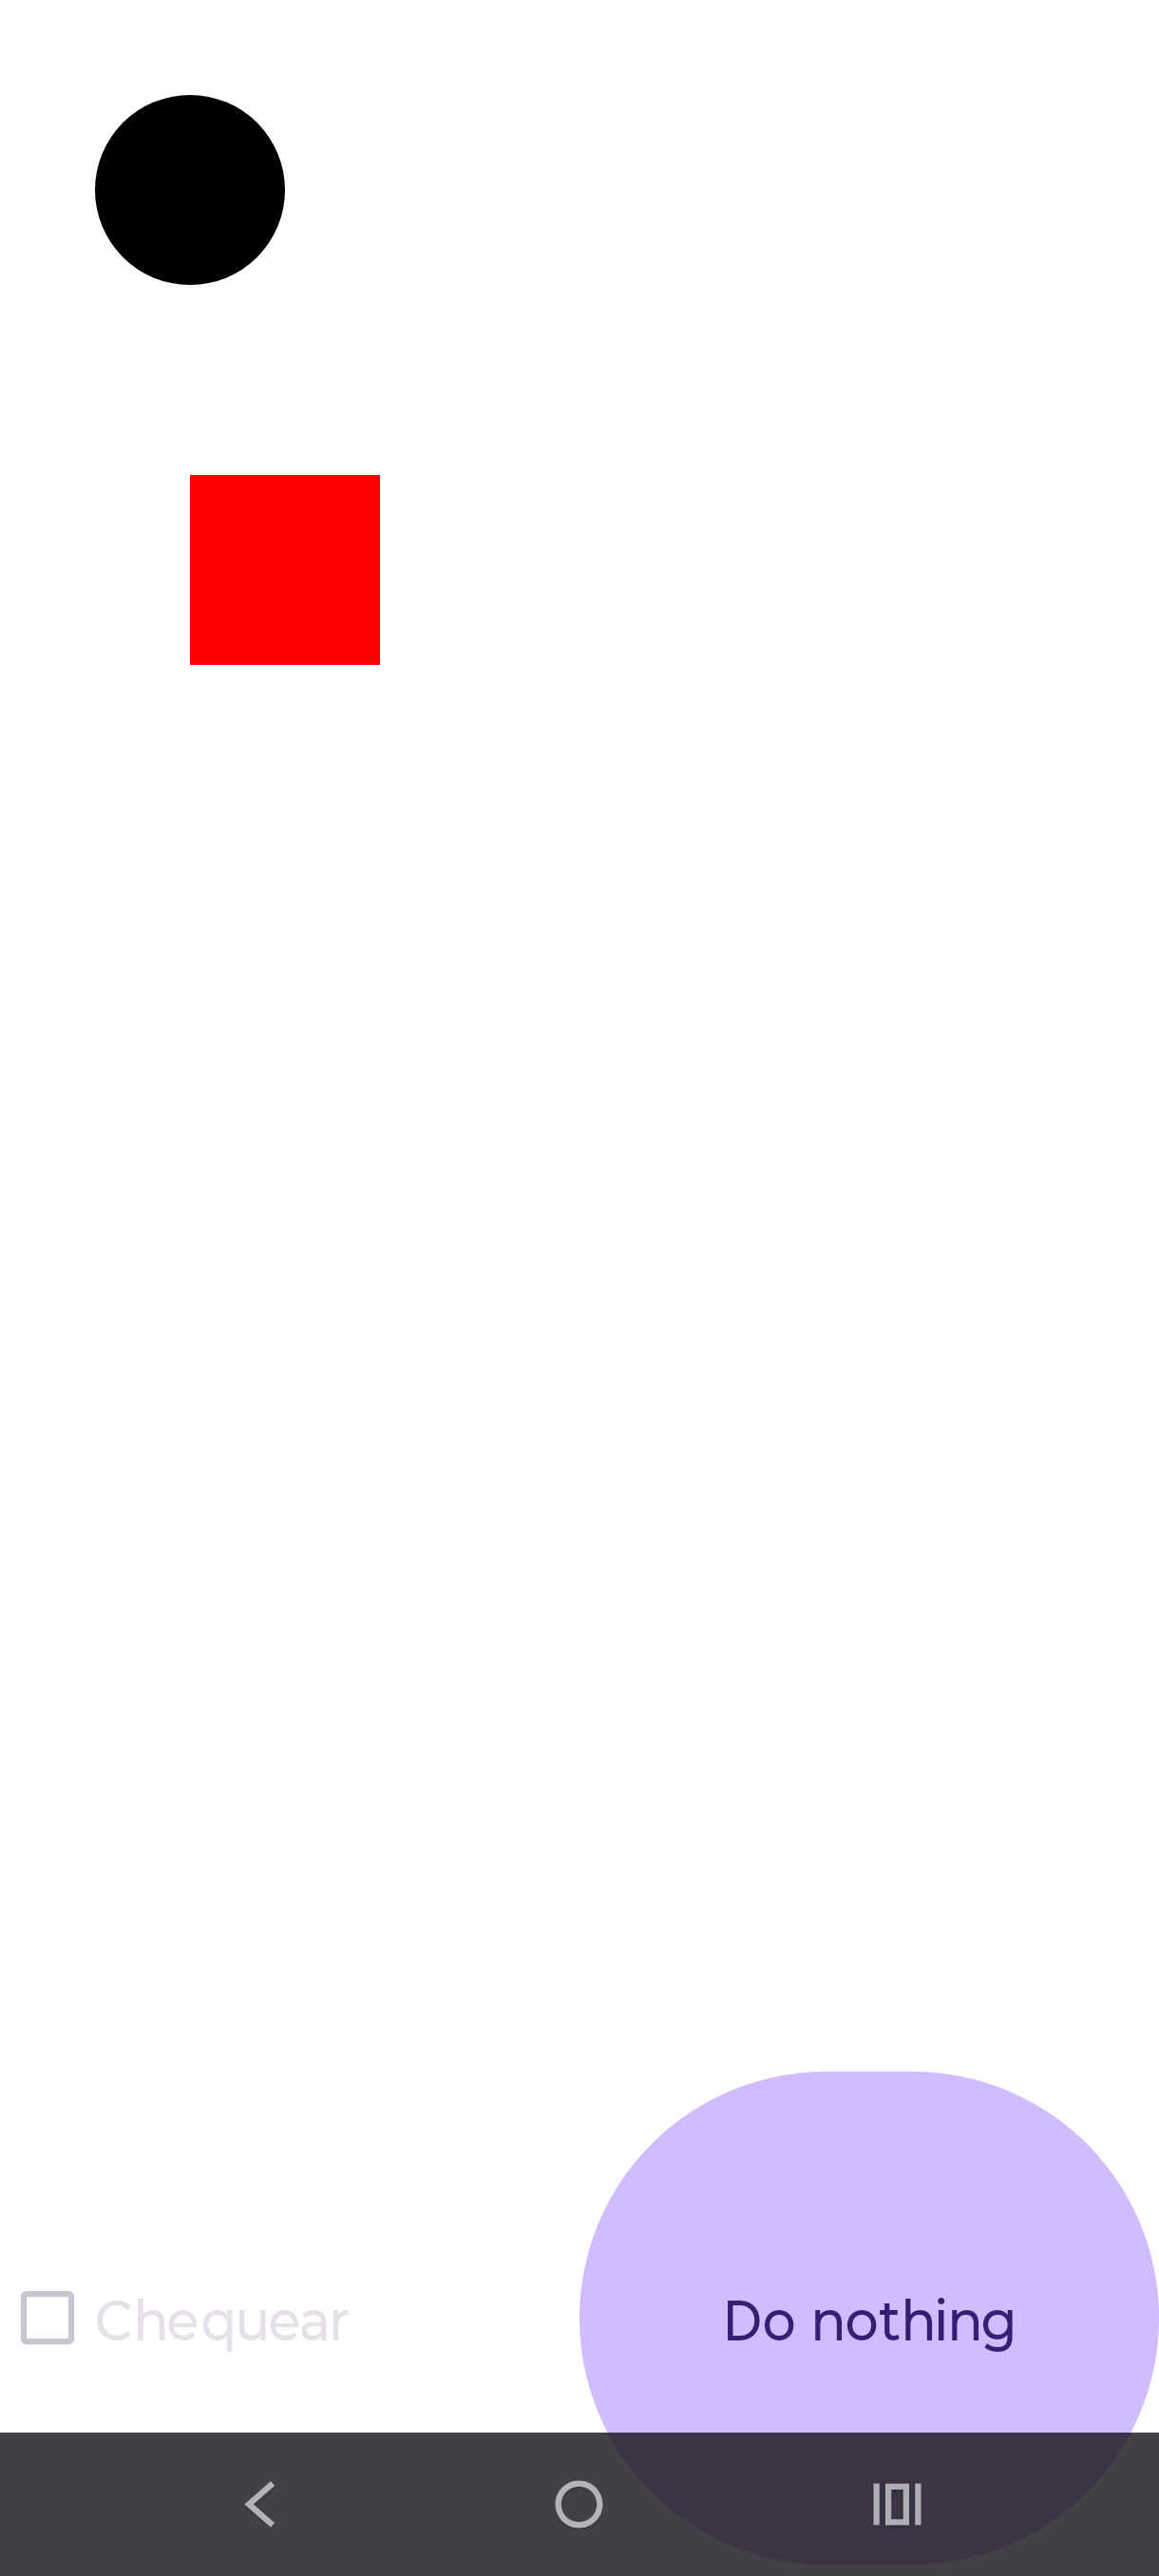
\includegraphics[width=0.98\textwidth]{02_TallerCBTis/figs/Demo17}
\end{center}

\end{columns}

\end{frame}



\begin{frame}[fragile]{Clase: MainActivity\_Demo18}

\begin{itemize}
    \item Es la actividad principal de la aplicación.
    \item Controla la interacción entre la interfaz y la lógica del juego.
\end{itemize}


\textbf{Componentes principales:}
\begin{itemize}
    \item \textbf{TicTacToeView:} Vista personalizada (probablemente basada en SurfaceView) para el juego.
    \item \textbf{Button (B1):} Botón para reiniciar el juego.
\end{itemize}


\textbf{Funcionamiento:}
\begin{itemize}
    \item En \texttt{onCreate()}:
    \begin{itemize}
        \item Se carga el layout con \texttt{setContentView()}.
        \item Se inicializa el botón con \texttt{findViewById()}.
        \item Se asigna un \texttt{OnClickListener}.
    \end{itemize}
    \item Al presionar el botón:
    \begin{itemize}
        \item Se invoca \texttt{resetGame()} en la vista.
        \item Se reinicia el estado del juego (tablero, movimientos, etc.).
    \end{itemize}
\end{itemize}

\
\end{frame}



\begin{frame}[fragile]
\frametitle{Demo 18: Tic-Tac-Toe }
\begin{columns}
\column{0.80\linewidth}

\scriptsize
Del Repositorio Github:
\begin{itemize}
%\item Agregar la siguiente linea: \textit{implementation("com.github.PhilJay:MPAndroidChart:v3.1.0")}, al final de la seccion Dependencies del archivo Build.graddle.kts (Module: App).
%\item Agregar la siguiente linea: \textit{maven \{ url = uri(``https://jitpack.io'') \}}, al final de la seccion \textit{dependencyResolutionManagement } del archivo settings.graddle.kts.
\item Copiar el archivo \textit{MainActivity\_Demo18.java} (dentro del Folder códigosJAVA) al mismo directorio donde esta el MainActivity.java
\item Copiar los archivos \textit{TicTacToeView.java},  (dentro del Folder códigosJAVA) al mismo directorio donde esta el MainActivity.java
\item Copiar el archivo \textit{activity\_main\_demo18.xml} (dentro del Folder Carpeta\_layout) al mismo directorio donde esta el activity\_main.xml
\item Modificar dentro del archivo \textit{activity\_main\_demo18.xml} la cadena \textit{.com.example.a2026\_01\_holamundoandroid.TicTacToeView} por \textit{$<$SuPackage$>$.TicTacToeView}.
\item Modificar en el archivo \textit{AndroidManifest.xml} la cadena \textit{.MainActivity\_Demo17} por \textit{.MainActivity\_Demo18}.


%\item Ir a la linea 22 de archivo del archivo \textit{MainActivity\_Demo09.java}, poner el cursos en la palabra (en Rojo) \textit{documentfile}, presionar la combinación ALT+ENTER, y seleccionar de la lista desplegable la opcion ``Add dependency on ....''. Esto quitará el error y hara los ajustes necesarios. 
\end{itemize}

%\begin{block}{Demo \#09}
%Un App que permite escribir el contenido de un EditText a un archivo y cargar el contenido de cualquier archivo en el EditText
%\end{block}


\column{0.20\linewidth}

\begin{center}
 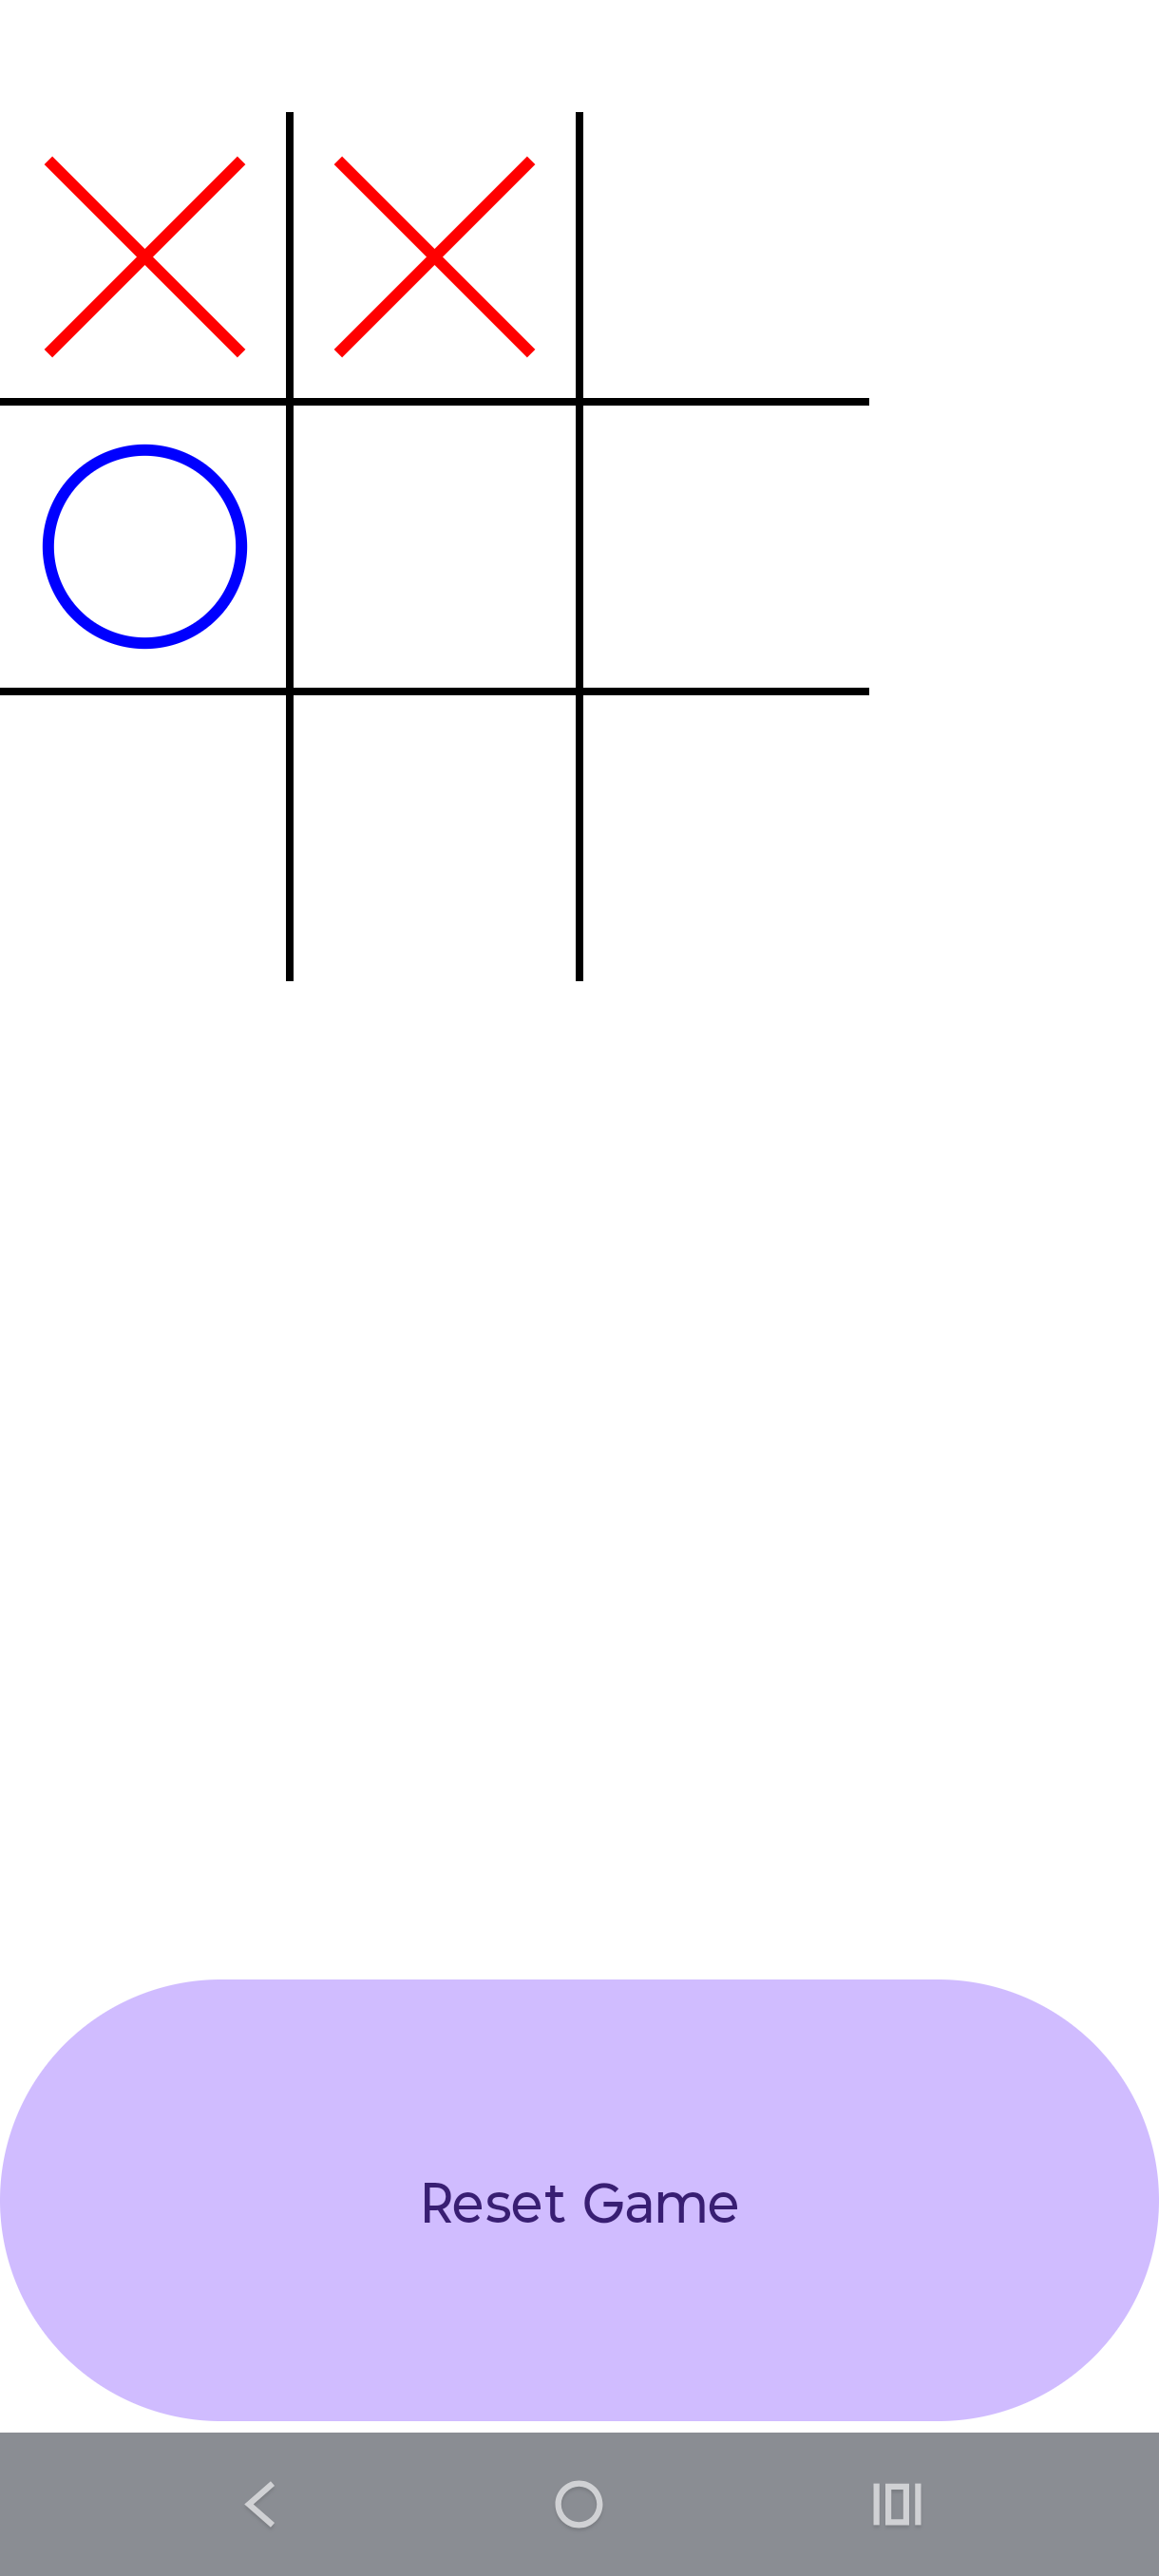
\includegraphics[width=0.98\textwidth]{02_TallerCBTis/figs/Demo18}
\end{center}

\end{columns}

\end{frame}


\begin{frame}[fragile]{Análisis de MainActivity\_Demo19}
\textbf{Clase: MainActivity\_Demo19}

\begin{itemize}
    \item Es la actividad principal de una aplicación Android.
    \item Extiende de \texttt{AppCompatActivity}.
    \item Se encarga de inicializar la interfaz y la vista del juego Pong (\textbf{PongSurfaceView:}).
\end{itemize}


\begin{itemize}
    \item En \texttt{onCreate()}:
    \begin{itemize}
        \item Se obtiene la referencia a \texttt{PongSurfaceView} con \texttt{findViewById()}.
		\item \textbf{Ciclo de vida:}
		\begin{itemize}
			\item \texttt{onResume()} y \texttt{onPause()} están definidos pero sin lógica adicional.
			\item Normalmente se usarían para pausar/reanudar el hilo del juego.
		\end{itemize}
    \end{itemize}
\end{itemize}

\textbf{Idea clave:}
\begin{itemize}
    \item La Activity actúa como contenedor, mientras que toda la lógica y renderizado del juego ocurre en \texttt{PongSurfaceView}.
\end{itemize}

\end{frame}


\begin{frame}[fragile]{Game Loop en PongSurfaceView (Android)}
\textbf{¿Qué es el Game Loop?}

\begin{itemize}
    \item Es un ciclo continuo que controla la ejecución de un videojuego.
    \item Se encarga de:
    \begin{itemize}
        \item Actualizar la lógica del juego.
        \item Dibujar los elementos en pantalla.
        \item Controlar la velocidad (FPS).
    \end{itemize}
\end{itemize}

\textbf{Implementación en SurfaceView:}
\begin{itemize}
    \item Se ejecuta en un hilo independiente del UI thread.
    \item Usa \textbf{SurfaceHolder} para dibujar sobre el \textbf{Canvas}.
\end{itemize}


\textbf{Métodos clave:}
\begin{itemize}
    \item \textbf{update():} Movimiento de pelota, colisiones, puntaje.
    \item \textbf{draw():} Dibujo en Canvas (paletas, pelota, fondo).
    \item \textbf{controlFPS():} Regula la velocidad del juego.
\end{itemize}


\textbf{Idea clave:}
\begin{itemize}
    \item El Game Loop permite animaciones fluidas y control total del juego en tiempo real.
\end{itemize}

\end{frame}



\begin{frame}[fragile]
\frametitle{Demo 19: Pong Game }
\begin{columns}
\column{0.80\linewidth}

\scriptsize
Del Repositorio Github:
\begin{itemize}
%\item Agregar la siguiente linea: \textit{implementation("com.github.PhilJay:MPAndroidChart:v3.1.0")}, al final de la seccion Dependencies del archivo Build.graddle.kts (Module: App).
%\item Agregar la siguiente linea: \textit{maven \{ url = uri(``https://jitpack.io'') \}}, al final de la seccion \textit{dependencyResolutionManagement } del archivo settings.graddle.kts.
\item Copiar el archivo \textit{MainActivity\_Demo19.java} (dentro del Folder códigosJAVA) al mismo directorio donde esta el MainActivity.java
\item Copiar los archivos \textit{TicTacToeView.java},  (dentro del Folder códigosJAVA) al mismo directorio donde esta el MainActivity.java
\item Copiar el archivo \textit{activity\_main\_demo19.xml} (dentro del Folder Carpeta\_layout) al mismo directorio donde esta el activity\_main.xml
\item Modificar dentro del archivo \textit{activity\_main\_demo19.xml} la cadena \textit{.com.example.a2026\_01\_holamundoandroid.PongSurfaceView} por \textit{$<$SuPackage$>$.PongSurfaceView}.
\item Modificar en el archivo \textit{AndroidManifest.xml} la cadena \textit{.MainActivity\_Demo18} por \textit{.MainActivity\_Demo19}.


%\item Ir a la linea 22 de archivo del archivo \textit{MainActivity\_Demo09.java}, poner el cursos en la palabra (en Rojo) \textit{documentfile}, presionar la combinación ALT+ENTER, y seleccionar de la lista desplegable la opcion ``Add dependency on ....''. Esto quitará el error y hara los ajustes necesarios. 
\end{itemize}

%\begin{block}{Demo \#09}
%Un App que permite escribir el contenido de un EditText a un archivo y cargar el contenido de cualquier archivo en el EditText
%\end{block}


\column{0.20\linewidth}

\begin{center}
 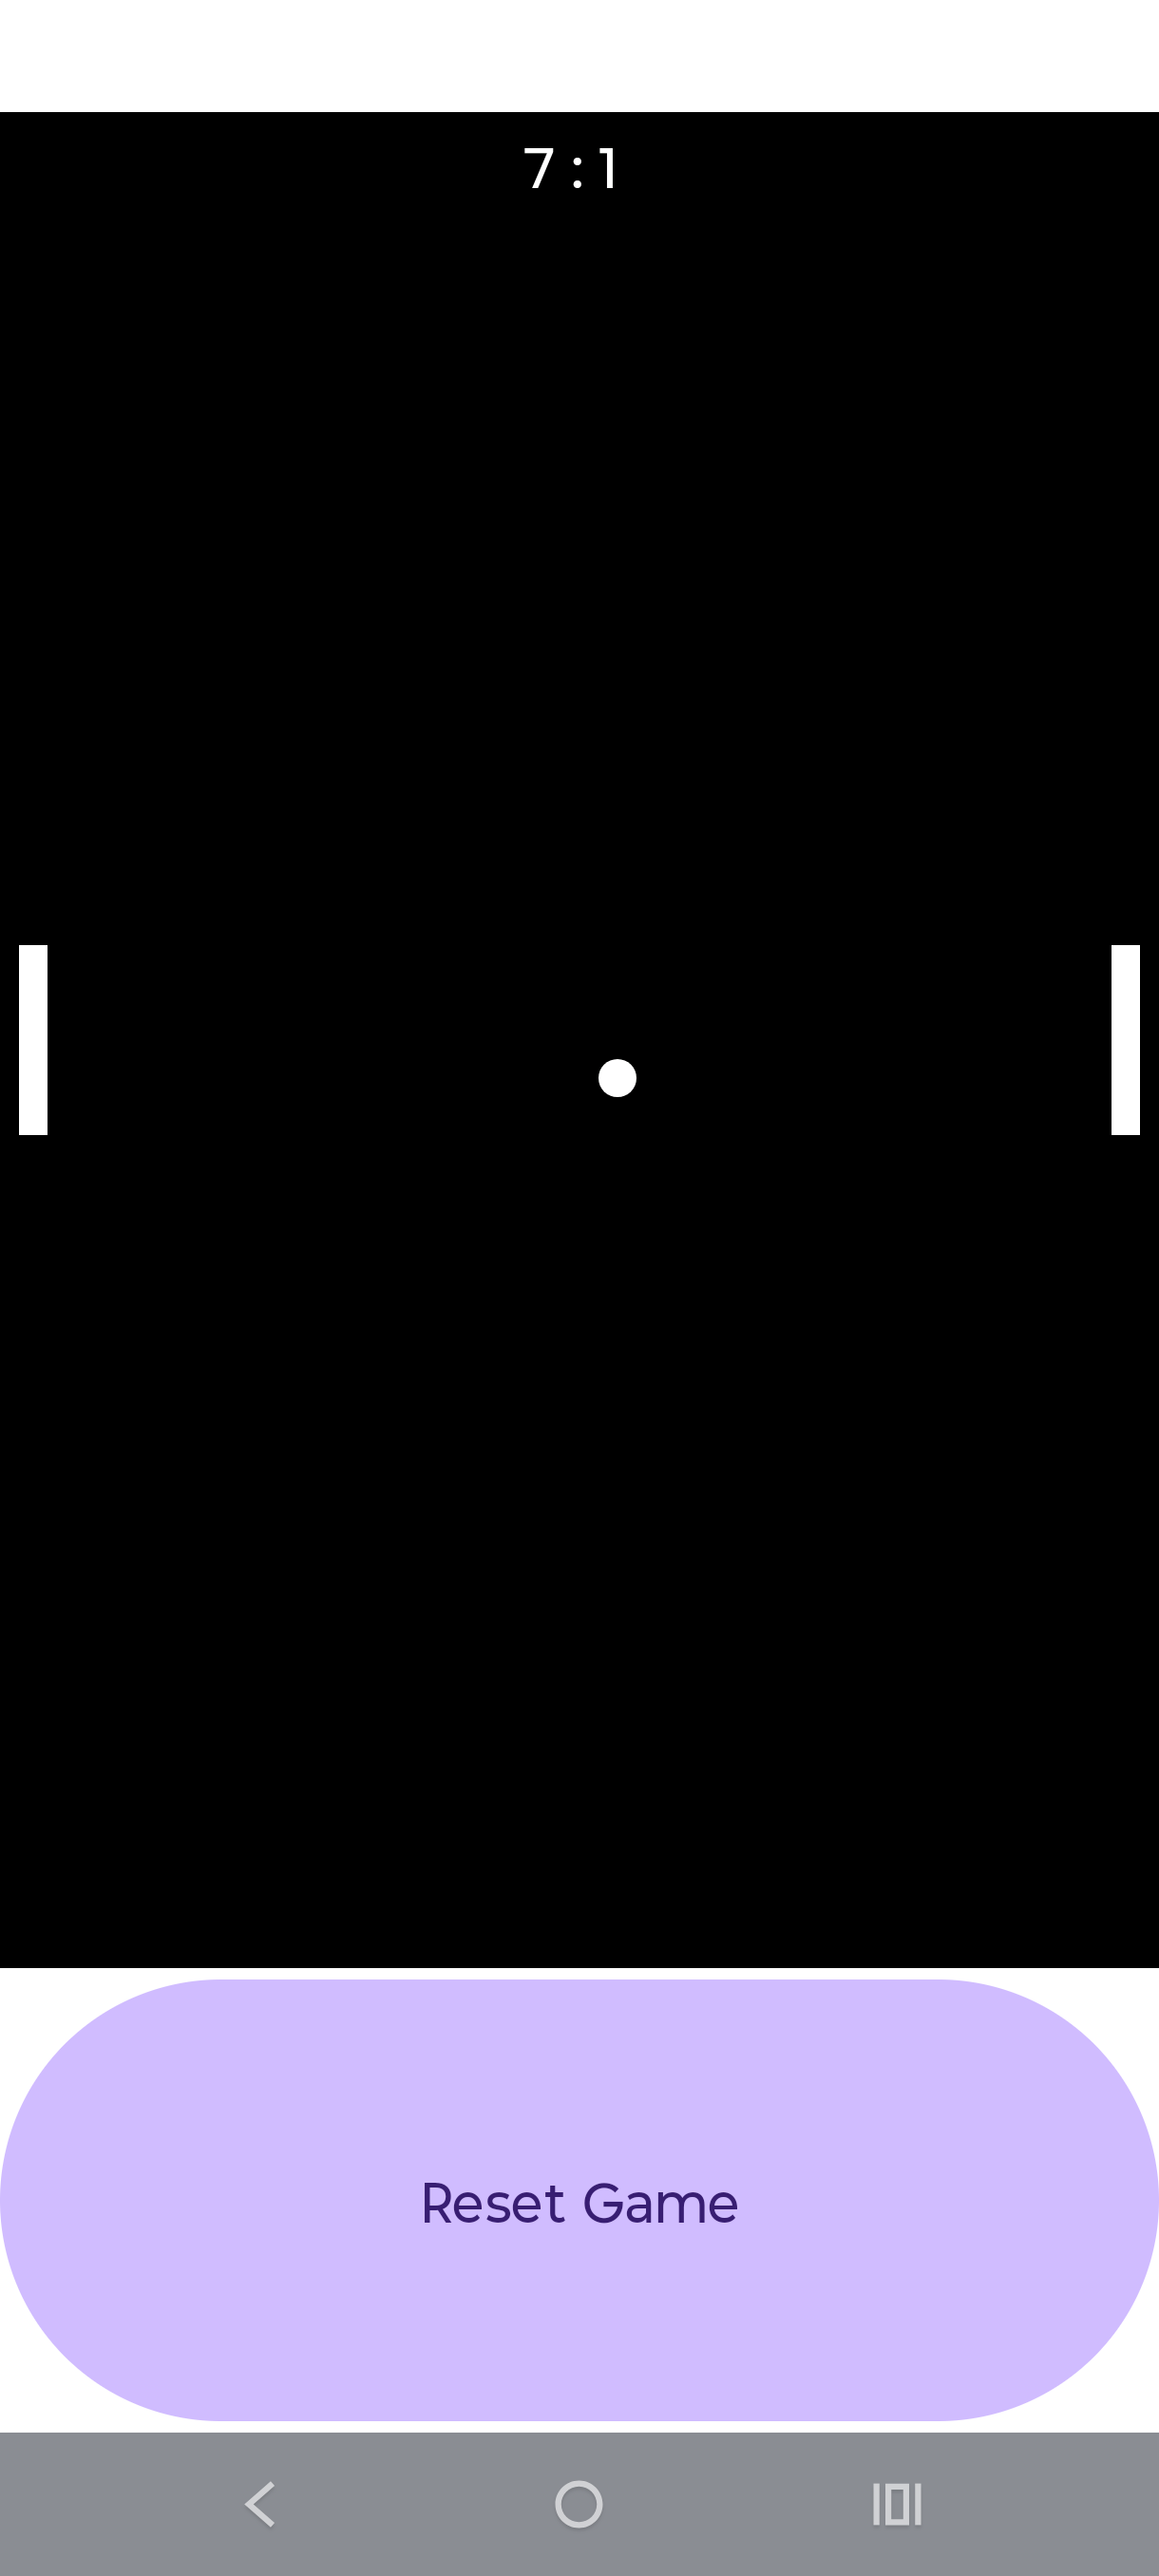
\includegraphics[width=0.98\textwidth]{02_TallerCBTis/figs/Demo19}
\end{center}

\end{columns}

\end{frame}


\begin{frame}[fragile]{Análisis de MainActivity\_Demo20}
\textbf{Propósito general:}

\begin{itemize}
    \item Implementa un menú basado en botones para navegar entre múltiples actividades (Demo01–Demo19).
    \item Utiliza un solo \textbf{OnClickListener} para manejar todos los eventos.
\end{itemize}


\textbf{Componentes principales:}
\begin{itemize}
    \item \textbf{Botones (B11–B54):} Representan una cuadrícula de opciones.
    \item \textbf{Tags:} Identificadores asociados a cada botón.
\end{itemize}


\textbf{Funcionamiento:}
\begin{itemize}
    \item Se asigna un \textbf{tag} a cada botón (\texttt{"11"}, \texttt{"12"}, ..., \texttt{"53"}).
    \item Un \textbf{listener común} captura el clic:
    \begin{itemize}
        \item Obtiene el tag del botón.
        \item Usa un \textbf{switch} para decidir qué Activity abrir.
        \item Lanza la nueva Activity con \texttt{Intent}.
    \end{itemize}
\end{itemize}

\textbf{Métodos auxiliares:}
\begin{itemize}
    \item \textbf{InicializarVistas():} Asocia variables con elementos XML.
    \item \textbf{InicializarTags():} Define identificadores para cada botón.
\end{itemize}

\end{frame}


\begin{frame}[fragile]
\frametitle{Demo 20: App Integradora }
\begin{columns}
\column{0.80\linewidth}

\scriptsize
Del Repositorio Github:
\begin{itemize}
%\item Agregar la siguiente linea: \textit{implementation("com.github.PhilJay:MPAndroidChart:v3.1.0")}, al final de la seccion Dependencies del archivo Build.graddle.kts (Module: App).
%\item Agregar la siguiente linea: \textit{maven \{ url = uri(``https://jitpack.io'') \}}, al final de la seccion \textit{dependencyResolutionManagement } del archivo settings.graddle.kts.
\item Copiar el archivo \textit{MainActivity\_Demo20.java} (dentro del Folder códigosJAVA) al mismo directorio donde esta el MainActivity.java
%\item Copiar los archivos \textit{TicTacToeView.java},  (dentro del Folder códigosJAVA) al mismo directorio donde esta el MainActivity.java
\item Copiar el archivo \textit{activity\_main\_demo20.xml} (dentro del Folder Carpeta\_layout) al mismo directorio donde esta el activity\_main.xml
%\item Modificar dentro del archivo \textit{activity\_main\_demo20.xml} la cadena \textit{.com.example.a2026\_01\_holamundoandroid.PongSurfaceView} por \textit{$<$SuPackage$>$.PongSurfaceView}.
\item Modificar en el archivo \textit{AndroidManifest.xml} la cadena \textit{.MainActivity\_Demo19} por \textit{.MainActivity\_Demo20}.


%\item Ir a la linea 22 de archivo del archivo \textit{MainActivity\_Demo09.java}, poner el cursos en la palabra (en Rojo) \textit{documentfile}, presionar la combinación ALT+ENTER, y seleccionar de la lista desplegable la opcion ``Add dependency on ....''. Esto quitará el error y hara los ajustes necesarios. 
\end{itemize}

Agregar en el archivo AndroidManifest, despues de $<$$\backslash$Activity$>$ lo siguiente: 
\begin{minted}[linenos,fontsize=\tiny]{xml}
<!-- ES necesario registar todas las actividades adicionales-->
        <activity android:name=".MainActivity_Demo01"></activity>
        <activity android:name=".MainActivity_Demo02"></activity>
...
        <activity android:name=".MainActivity_Demo19"></activity>
\end{minted}


%\begin{block}{Demo \#09}
%Un App que permite escribir el contenido de un EditText a un archivo y cargar el contenido de cualquier archivo en el EditText
%\end{block}


\column{0.20\linewidth}

\begin{center}
 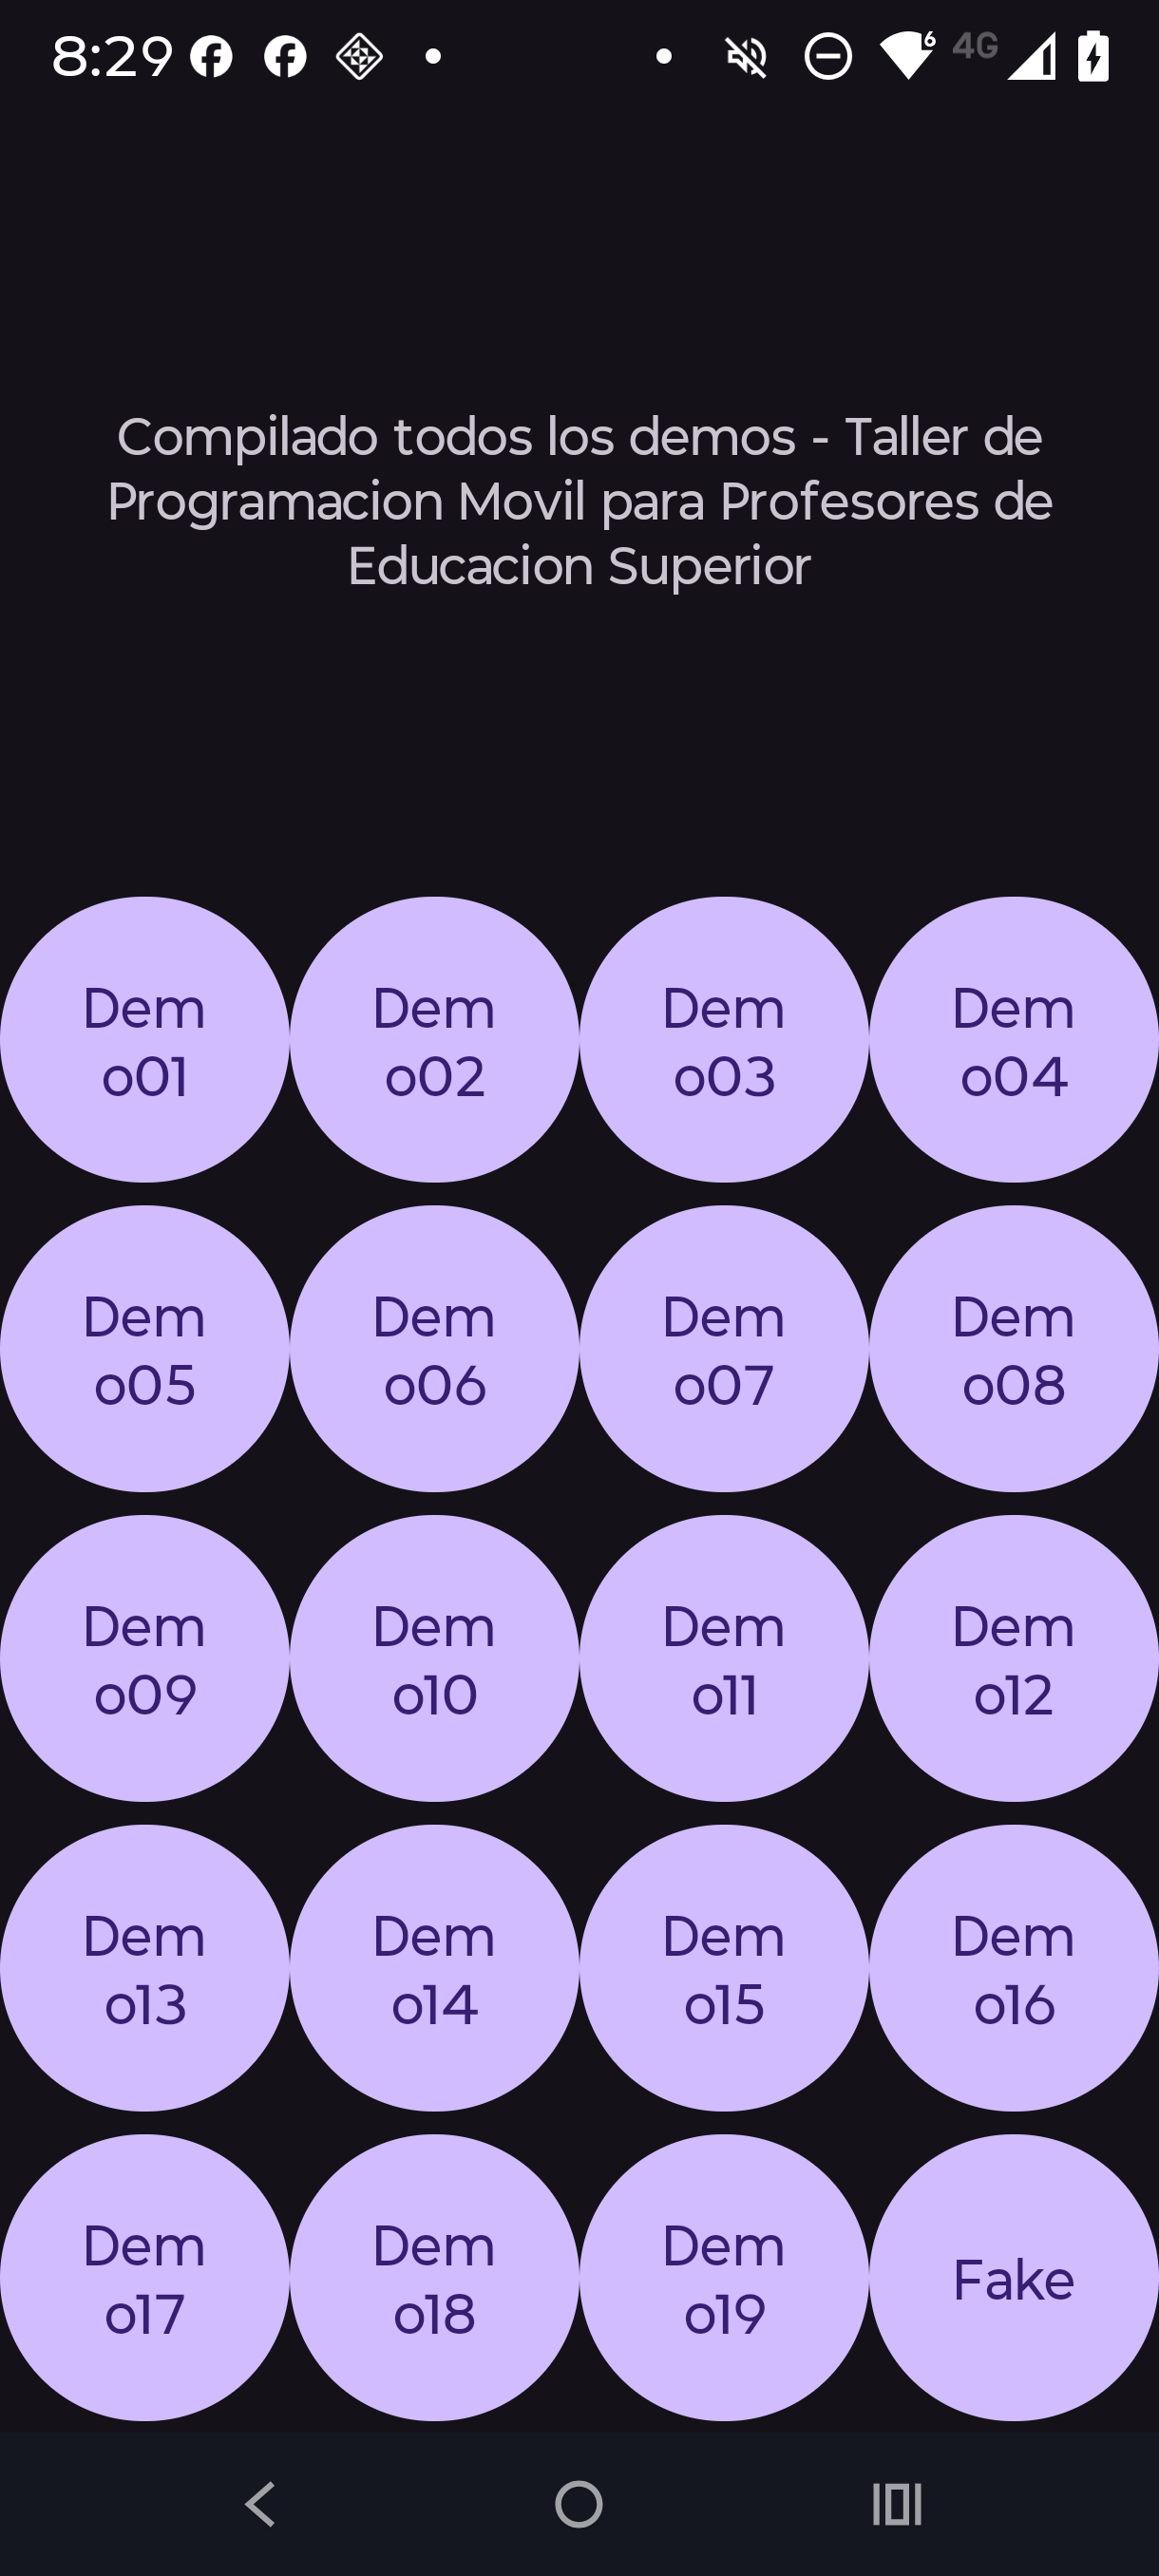
\includegraphics[width=0.98\textwidth]{02_TallerCBTis/figs/Demo20}
\end{center}

\end{columns}

\end{frame}




\section[CP1]{Conclusiones}
\begin{frame}{Conclusiones}
En este taller:
\begin{itemize}
\item Se explicaron los conceptos de Telefono Inteligente, Sistema Operativo.
\item Se describieron los materiales necesarios (hardware y software) para la implementacion de una app en Android.
\item Se revisaron los principales componentes de interfaz grafica y su uso en Apps de Android Studio. 
\item Se pusieron en practica aplicaciones simples que emplean componentes de interfaz grafica, manejo de archivos y librerias externas para propositos misceláneos. 

\end{itemize}
\end{frame}

\begin{frame}%%     2
\begin{center}
{\fontsize{40}{50}\selectfont ¡Gracias!}
\end{center}
Comentarios o Dudas: mnunom@upv.edu.mx 
\end{frame}


\end{document}





\begin{frame}
\frametitle{Agradecimiento}  
%Se agradece al Consejo Tamaulipeco de Ciencia y Tecnologia (COTACYT) por la invitaci\'on a este evento

%Comentarios o Dudas: mnunom@upv.edu.mx 
\end{frame}


\end{document}


%\input{00_DispositivosVR/DispositivosVR.tex}

%\section[HR]{Herramientas Requeridas}
%\input{00_AndroidStudio/AndroidStudio.tex}
%\input{00_HerramientasParaTallerGraficos/Herramientas.tex}



%\section[Intro]{Conceptos}
%Parte 1: Conceptos
%\input{00_IntroAI/IntroAI.tex}
%* Vision por Computadora
%\input{00_IntroComputerVisionV2/IntroVC.tex}
%* Graficos por Computadora
%\input{00_IntroGC/IntroGC.tex}
%* Realidad Virtual
%\input{00_IntroAR_VR/IntroAR_VR.tex}
%* Realidad Aumentada
%Parte 2: Intro a Telefonos Moviles
%\section[Tools]{Herramientas}
%* Android y SO para smartphones
%\input{00_IntroProgramacionMovil/IntroPM.tex}
%* Tomada del Taller del CBTIS

%\section[PCS]{Pasos para configurar Smartphone}
%\input{01_Configurar/Configurar.tex}

%\input{01_PasosCrearProyectoAndroidStudio/Pasos.tex}

%\section[PDAS]{Primer demo en Android Studio}

%\input{01_Modificacion/Modificacion0.tex}

%\section[PRVA]{Prototipos de Aplicaciones Graficas y de VC}

%\input{2017_Ajedrez3D/Ajedrez3D.tex}
%\input{2017_CruzdeMalta/CruzDeMalta.tex}
%\input{2017_Tetris3D/Tetris3D.tex}
%\input{2022_FatChild3D/T20.tex}
%\input{2019_BrazoRobot3D/BrazoRobot3D.tex}




%----A) Software (Android Studio, Scrcpy, Blender, Gimp, UNITY)
%----B) Hardware: Adaptador, Cable USB, Control de Juegos Bluetooth
%Parte 3: Android Studio
%* Creacion de proyectos en Android (Taller de Moviles CBTIS 236)
%* Herramienta ADB para instalar APKs existentes (Taller de Moviles CBTIS 236)
%* Hola Mundo Android (Juego del Gato)  (Simplificacion de Taller de Moviles CBTIS 236)
%* Hola Mundo Android OpenGL ES (Triangulos)
%* Hola Mundo Android OpenCV (Segmentar Color)
%Parte 4: OpenGL ES Primitivas (y sus respectivos demos) - Taller OpenGL
%* Cubo, Circulo, Cilindro, Esfera, Texturas, etc (Demos 1 a 7 del Taller de OpenGL)
%Parte 5: Realidad Aumentada
%* Demo del CUBO con OpenCV (Clases)
%* Demo del Jaguar de la UPV (Libreria Rajawali)
%* Version minima del Demo del Tigre/Mapa de la UPV
%* APK Mapa de la UPV
%Parte 6: Realidad Virtual
%** Version minima del Mapa de la UPV
%** APK Mapa de la UPV
%Parte 7: Conclusiones


\section[CP1]{Conclusiones}
\begin{frame}{Conclusi\'on}
\begin{itemize}
\item Se present\'o la relaci\'on entre Inteligencia Articial, Visi\'on por Computadora y los Gr\'aficos por Computadora con la RA y la RV
\item Se establecieron las herramientas Hardware y Software para Realizar proyectos Gr\'aficos y de RA y RV para Tel\'efonos Inteligentes en Android Studio
\item Se presentaron proyectos de Graficaci\'on y de RA y RV, principalmente desarrollados por estudiantes de la UPV (Ingenier\'ia en Tecnolog\'ias de la Informaci\'on y de Maestría en Ingeniería)
%\item Algunos trabajos establecen vínculos de colaboracion con otras universidades
\end{itemize}
\end{frame}





\renewcommand*{\bibfont}{\tiny}
\begin{frame}[allowframebreaks]{Artículos publicados}
    \printbibliography[title=Artículos publicados,keyword=primary]
\end{frame}

\end{document}


  



\end{document}


